% !TEX spellcheck=en_US
\documentclass[a4paper]{article}
\usepackage[american]{babel}
\usepackage[T1]{fontenc}
\usepackage[utf8]{inputenc}
\usepackage[activate={true,nocompatibility},final,tracking=true,kerning=true,spacing=true,factor=1100,stretch=10,shrink=10]{microtype}
\usepackage{graphicx}
\usepackage[table,dvipsnames]{xcolor}
\usepackage{caption}
\usepackage{subcaption}
\usepackage{csquotes}
\usepackage{hyperref}
\usepackage{url}
\usepackage[super]{nth}
\usepackage{amsmath}
\usepackage{amssymb}
\usepackage{amsthm}
\usepackage{mathtools}
\usepackage{mathmacros/mathmacros}
\usepackage{tcolorbox}
\usepackage{circuitikz}
\usepackage{tikz}
\usepackage{pgf}
\usepackage{pgfplots}
\usepackage[acronym]{glossaries}
\usepackage[backend=biber,style=phys]{biblatex}

% environments
\newtheorem{lemma}{Lemma}
\newtheorem{thm}{Theorem}
\newtheorem{crl}{Corollary}
\newtheorem{definition}{Definition}
\theoremstyle{remark}
\newtheorem{exm}{Example}
\theoremstyle{remark}
\newtheorem{rem}{Remark}

% misc macros
\newcommand*{\pref}[2]{#1 (\ref{#2})}
\definecolor{lightgray}{rgb}{0.9725,0.9725,0.9725}

% microtype
\SetTracking{encoding={*}, shape=sc}{0}

% pgfplots
\pgfplotsset{compat=newest}

\addbibresource{bibliography.bib}

\makenoidxglossaries
\newacronym{dne}{DNE}{does not exist}
\newacronym{pfd}{PFD}{partial fraction decomposition}
\newacronym{wlog}{WLOG}{without loss of generality}

% mathematicians
\newcommand*{\lhoptial}{L'H{\^o}pital}

\begin{document}

\begin{titlepage}
	\centering
	{\scshape\Huge \bfseries{Advanced Systems} \par}
	\par\vspace{1cm}
	\includegraphics[width=0.45\textwidth]{images/logo.png}\par
	\vspace{3cm}
	{\huge\bfseries Lecture Notes \par}
	\vspace{1cm}
	{\LARGE\itshape Mazawa Shinonome \par}
	\vspace{1cm}
	{\large\today\par}
	\vfill
	\begin{abstract}
		This document is a compilation of lecture notes for intermediate mathematics.
		It is intended to serve as a study guide for members of the Advanced System
		organization.
	\end{abstract}
\end{titlepage}

\newpage

\microtypesetup{protrusion=false}
\clearpage
\printnoidxglossaries
\newpage
\tableofcontents
\microtypesetup{protrusion=false}

\newpage

% === Begin Section Includes ===

\section{Acknowledgements}

\begin{flushleft}
	In this section of the draft I would like to express my very great appreciation
	to Dr. Aviv Censor from the Israel Institute of Technology, Prof. Jhevon Smith
	from the Mathematics department at Fordham University and Prof. David Massey
	from the Northeastern University. This document would not have been possible
	without their lectures whose recordings they made accessible to a public audience
	on YouTube. Additional references are listed in the bibliography.
\end{flushleft}

\begin{flushleft}
	The \hyperref[sec-lina]{first} section closely follows Dr. Aviv Censor's
	(linear) algebra lecture\cite{algebraCensor2015}. The \hyperref[sec-analysis]{second}
	and \hyperref[sec-single-var-calc]{third} section are a combination of Dr. Aviv
	Censor's \cite{calc1Censor2015} and Prof. David Massey's lectures on single
	variable calculus. Building on this, the \hyperref[sec-multi-var-calc]{fourth}
	section is a transcription of Prof. Jhevon Smith's \cite{vectorCalcSmith2018}
	lecture series on multi-variable calculus.
\end{flushleft}


\section{Introduction}

\begin{flushleft}
	The Advanced System organization is an open-source software community who's main
	purpose it is to develop modern and user-friendly utility programs. In order to
	develop advanced applications, the study of mathematics is of particular interests:
	It lays the groundwork for many other fields of studies such as physics or computer
	science.
\end{flushleft}

\begin{flushleft}
	While this document has been drafted with the best intents and purposes, there
	is no warranty on the correctness of its content. You can find the source code
	on \url{www.github.com/Advanced-Systems/lecture-notes} to compile a new PDF
	file from scratch using the most recent version of this document or raise an
	issue to report mistakes under the issues tab of GitHub.
\end{flushleft}


\section{Analysis}\label{sec-analysis}

TODO: Add description


\section{Logic}

% ==============================================================================
% ==============================================================================
% ==============================================================================

\subsection{Truth Tables}\label{subsec-truth-table}

% TODO: Add description and explanation here (T=1, F=0)

\begin{table}[hbt!]
    \centering
    \rowcolors{1}{}{lightgray}
    \begin{tabular}{*{6}{c}}
        $(A$ & $\land$ & $B)$ & $\rightarrow$ & $C$ \\
           T &         & T    &               & T   \\
           T &         & F    &               & T   \\
           F &         & T    &               & F   \\
           F &         & F    &               & F   \\
    \end{tabular}
    \caption{Conjunction}\label{table-conjunction}
\end{table}

\begin{table}[hbt!]
    \centering
    \rowcolors{1}{}{lightgray}
    \begin{tabular}{*{6}{c}}
        $(A$ & $\lor$ & $B)$ & $\rightarrow$ & $C$ \\
           T &        & T    &               & T   \\
           T &        & F    &               & T   \\
           F &        & T    &               & T   \\
           F &        & F    &               & F   \\
    \end{tabular}
    \caption{Disjunction}\label{table-disjunction}
\end{table}

\begin{table}[hbt!]
    \centering
    \rowcolors{1}{}{lightgray}
    \begin{tabular}{*{6}{c}}
        $(A$ & $\Rightarrow$ & $B)$ & $\rightarrow$ & $C$ \\
           T &               & T    &               & T   \\
           T &               & F    &               & F   \\
           F &               & T    &               & T   \\
           F &               & F    &               & T   \\
    \end{tabular}
    \caption{Subjunction}\label{table-subjunction}
\end{table}

\begin{table}[hbt!]
    \centering
    \rowcolors{1}{}{lightgray}
    \begin{tabular}{*{6}{c}}
        $(A$ & $\Leftrightarrow$ & $B)$ & $\rightarrow$ & $C$ \\
           T &                   & T    &               & T   \\
           T &                   & F    &               & F   \\
           F &                   & T    &               & F   \\
           F &                   & F    &               & T   \\
    \end{tabular}
    \caption{Bisubjunction}\label{table-bisubjunction}
\end{table}

\begin{table}[hbt!]
    \centering
    \rowcolors{1}{}{lightgray}
    \begin{tabular}{*{6}{c}}
        $(\neg$ & $B)$ & $\rightarrow$ & $C$ \\
                & T    &               & F   \\
                & F    &               & T   \\
    \end{tabular}
    \caption{Negation}\label{table-negation}
\end{table}

% ==============================================================================
% ==============================================================================
% ==============================================================================

\subsection{Circuit Representation of Logical Operations}\label{subsec-circuits}

Truth tables are very useful in determining the nature of logic gates.
In \pref{Table}{subsec-truth-table} find defined the axioms which build the basis for
this section. Take \texttt{XOR}, for instance: this logic gate evaluates to $1$
if and only if one of both poles receives $1$ as an input as opposed to \texttt{OR}
which also accepts two positive-valued states favorably.

\begin{table}[hbt!]
    \centering
    \rowcolors{1}{}{lightgray}
    \begin{tabular}{*{6}{c}}
        $A$ & $B$ & $A\texttt{ OR }B$ & $A\texttt{ AND }B$ & $A\texttt{ NAND }B$ & $(A\texttt{ OR }B)\texttt{ AND }(A\texttt{ NAND }B)$ \\
          1 & 1   & 1                 & 1                  & 0                   & 0                                                    \\
          1 & 0   & 1                 & 0                  & 1                   & 1                                                    \\
          0 & 1   & 1                 & 0                  & 1                   & 1                                                    \\
          0 & 0   & 0                 & 0                  & 1                   & 0                                                    \\
    \end{tabular}
    \caption{\texttt{XOR} Truth Table}\label{truth-table-xor}
\end{table}

Based on this truth table it is possible to implement a logic gate that replicates
a \texttt{XOR} gate in the following way:

\begin{figure}[hbt!]
    \centering
    \begin{circuitikz}
        % gates
        \node[or port,draw] at (0,2) (or) {};
        \node[nand port,draw] at (0,0) (nand) {};
        \node[and port,draw] at (2,1) (and) {};
        % inputs
        \node at ($(or.in 1) + (-1,0)$) (A) {$A$};
        \node at ($(nand.in 2) + (-1,0)$) (B) {$B$};
        % wires
        \draw (A) -- (or.in 1);
        \draw (A) -- (nand.in 1);
        \draw (B) -- (or.in 2);
        \draw (B) -- (nand.in 2);
        \draw (or.out) -- (and.in 1);
        \draw (nand.out) -- (and.in 2);
        \draw (and.out) -- ($(and.out) + (0.5,0)$) node[anchor=west] (Q) {$Q$};
    \end{circuitikz}
    \caption{Circuit of an \texttt{XOR} gate}\label{circuit-xor-gate}
\end{figure}

A half adder is a circuit that adds two binary numbers, each one bit in size.
The result $S$ is also represented by a one bit value, so in case of 
$1_2+1_2=(10)_2$ the second digit must be carried over in $C$ (hence the name 
\textit{carrier}) in order to be preserved for future operations.

\begin{figure}[hbt!]
    \centering
    \begin{circuitikz}
        % xor gate
        \node[xor port,draw] at (0,2) (xor) {};
        \draw (xor.in 1) -- ($(xor.in 1) + (-0.75,0)$) node[anchor=east] (A) {$A$};
        \draw (xor.in 2) -- ($(xor.in 2) + (-0.75,0)$) node[anchor=east] (B) {$B$};
        \draw (xor.out) -- ($(xor.out) + (0.75,0)$) node[anchor=west] (S) {$S$};
        % and gate   
        \node[and port,draw] at (0,0) (and) {};
        \draw (xor.in 1) -- (and.in 1);
        \draw ($(xor.in 2) + (-0.25,0)$) -- ($(and.in 2) + (-0.25,0)$) -- (and.in 2);
        \draw (and.out) -- ($(and.out) + (0.75,0)$) node[anchor=west] (C) {$C$};        
    \end{circuitikz}
    \caption{Circuit of an half adder}\label{circuit-half-adder}
\end{figure}

\begin{table}[hbt!]
    \centering
    \rowcolors{1}{}{lightgray}
    \begin{tabular}{*{4}{c}}
        $A$ & $B$ & $S$ & $C$ \\
          1 & 1   & 0  & 1    \\
          1 & 0   & 1  & 0    \\
          0 & 1   & 1  & 0    \\
          0 & 0   & 0  & 0    \\
    \end{tabular}
    \caption{Half Adder Truth Table}\label{truth-table-half-adder}
\end{table}

As opposed to an half adder, a full adder takes one more input (a so-called \texttt{carry in})
and two outputs, \textit{i.e.} \texttt{carry out} and \texttt{sum}. To build a
more sophisticated adder, chain half adders in a way that allows the result of
the previous sum to be carried over as \texttt{cin} to the next half adder.

\begin{figure}[hbt!]
    \centering
    \begin{circuitikz}
        % gates
        \node[xor port,draw,anchor=center] at (0,4) (xor1) {D};
        \node[xor port,draw] at (2,4) (xor2) {};
        \node[and port,draw] at (2,2) (and1) {E};
        \node[and port,draw] at (2,0) (and2) {F};
        \node[or port,draw] at (4,1) (or) {};
        % inputs
        \node at ($(xor1.in 1) + (-1,0)$) (A) {$A$};
        \node at ($(xor1.in 2) + (-1,0)$) (B) {$B$};
        \node at ($(A) + (0,-1.5)$) (C) {$C_{in}$};
        % wires
        \draw (A) -- (xor1.in 1);
        \draw (B) -- (xor1.in 2);
        \draw (xor1.out) -- (xor2.in 1);
        \draw (C) -- (xor2.in 2);
        \draw (C) -- (and1.in 1);
        \draw (xor1.out) -- ($(and1.in 2)-(0.5,0)$) -- (and1.in 2);
        \draw ($(A)+(0.75,0)$) -- ($(A)+(0.75,-4.56)$) -- (and2.in 2);
        \draw ($(B)+(1,0)$) -- ($(B)+(1,-3.425)$) -- (and2.in 1);
        \draw (and1.out) -- (or.in 1);
        \draw (and2.out) -- (or.in 2);
        \draw (xor2.out) -- ($(xor2.out) + (0.5,0)$) node[anchor=west] (S) {$S$};
        \draw (or.out) -- ($(or.out) + (0.5,0)$) node[anchor=west] (Q) {$C_{out}$};
    \end{circuitikz}
    \caption{Circuit of an full adder}\label{circuit-full-adder:1}
\end{figure}

Circuit (\ref{circuit-full-adder:1}) introduced three additional truth values 
to make the truth table (\ref{truth-table-full-adder}) for the full adder easier
to read\footnote{Note that $S:\Leftrightarrow D\texttt{ XOR } C_{in}$ and 
$C_{out} :\Leftrightarrow E\texttt{ OR }F$}. It is helpful to think of gate $D$
and gate $F$ as the first half adder.

\begin{table}[hbt!]
    \centering
    \rowcolors{1}{}{lightgray}
    \begin{tabular}{*{8}{c}}
        $A$ & $B$ & $C_{in}$ & $A\texttt{ XOR }B$ & $D\texttt{ XOR }C_{in}$ & $D\texttt{ AND }C_{in}$ & $F$ & $E\texttt{ OR }F$ \\
          1 & 1   & 1        & 0                  & 1                       & 0                       & 1   & 1                 \\
          1 & 1   & 0        & 0                  & 0                       & 0                       & 1   & 1                 \\
          1 & 0   & 1        & 1                  & 0                       & 1                       & 0   & 1                 \\
          0 & 1   & 1        & 1                  & 0                       & 1                       & 0   & 1                 \\
          1 & 0   & 0        & 1                  & 1                       & 0                       & 0   & 0                 \\
          0 & 1   & 0        & 1                  & 1                       & 0                       & 0   & 0                 \\
          0 & 0   & 1        & 0                  & 1                       & 0                       & 0   & 0                 \\
          0 & 0   & 0        & 0                  & 0                       & 0                       & 0   & 0                 \\
    \end{tabular}
    \caption{Full Adder Truth Table}\label{truth-table-full-adder}
\end{table}


\section{Sets}\label{sec-sets}

% ==============================================================================
% ==============================================================================
% ==============================================================================

.....

\subsection{Indicator Functions}\label{subsec-indicator-functions}

\begin{definition}\label{def-indicator-function}
    Let $X$ be a set. For each subset $A \subseteq X$ there is defined the 
    indicator function\footnote{Sometimes, the term characteristic function is 
    used to describe the function that indicates membership in a set in other 
    fields of mathematics. The term indicator function is more prominently used 
    in probability theory.} $\chi_A:X\rightarrow \{0,1\}$ of the set $A$ as
    \begin{equation}
        \chi_A(x) = \begin{cases}
            1,\;\text{ if } x \in A \\
            0,\;\text{ if } x \notin A
        \end{cases}
    \end{equation}
    We will write $\chi_A$ instead of $\chi_A(x)$ if the parameter
    $x$ is unambiguous.
\end{definition}

\begin{thm}\label{thm-complement-indicator-function}
    Let $\chi_A$ be an indicator function. Then the complement of $A$ (i.e. 
    $\overline{A} \defines A^C$) is
    \begin{equation*}
        \chi_{\overline{A}} = 1 - \chi_A
    \end{equation*}
\end{thm}

\begin{proof}
    Of \pref{theorem}{thm-complement-indicator-function}.
    \begin{align*}
        \chi_{\overline{A}}(x) &= \begin{cases}
            1,\;\text{ if } \neg(x \in A) \\
            0,\;\text{ if } \neg(x \notin A)
        \end{cases} \\
        &= \begin{cases}
            1-0,\;\text{ if } x \notin A \\
            1-1,\;\text{ if } x \in A
        \end{cases} \\
        &=1 - \begin{cases}
            0,\;\text{ if } x \notin A \\
            1,\;\text{ if } x \in A
        \end{cases} \\
        &= 1 - \chi_A(x)
    \end{align*}
\end{proof}

\begin{thm}\label{thm-set-cardinality-indicator-function}
    Let $\chi_A$ be an indicator function with $A$ as a finite set. Then,
    \begin{equation*}
        \abs{A} = \sum_{x \in X} \chi_A(x)
    \end{equation*}
\end{thm}

\begin{proof}
    Of theorem (\ref{thm-set-cardinality-indicator-function}).
    \begin{align*}
        \abs{A} &=\sum_{x\in A}\underbrace{\chi_A(x)}_{1}\\
                &=\sum_{x\in A}\chi_A(x)+\sum_{x\in X\setminus A}\underbrace{\chi_A(x)}_{0}\\
                &=\sum_{x\in (A\cup (X\setminus A))}\chi_A(x)\\
                &\overset{(\star)}{=}\sum_{x\in X}\chi_A(x).
    \end{align*}
    since 
    \begin{equation*}
        (\star) :\Leftrightarrow A\cup(X\setminus A)=(A\cup X)\setminus(A\setminus A)=X\setminus \emptyset=X
    \end{equation*}
\end{proof}

\begin{thm}\label{thm-cap-indicator-function}
    Let $\chi_A,\chi_B$ be indicator functions. Then:
    \begin{equation*}
        \chi_{A \cap B} = \chi_A\chi_B
    \end{equation*}
\end{thm}

\begin{proof}
    Of \pref{theorem}{thm-cap-indicator-function}.
    \begin{align*}
        \chi_{A \cap B} &= \begin{cases}
            1\;\text{ if } x \in (A \cap B)\\
            0\;\text{ if } x \notin (A \cap B)
        \end{cases}\\
        &= \begin{cases}
            1\;\text{ if } x \in A \land x \in B\\
            0\;\text{ if } x \notin A \land x \notin B
        \end{cases}\\
        &= \left(\begin{cases}
            1\;\text{ if } x \in A\\
            0\;\text{ if } x \notin A
        \end{cases}\right)\left(\begin{cases}
            1\;\text{ if } x \in B\\
            0\;\text{ if } x \notin B
        \end{cases}\right)\\
        &= \chi_A\chi_B
    \end{align*}
\end{proof}

\begin{thm}\label{thm-cup-indicator-function}
    Let $\chi_A,\chi_B$ be indicator functions. Then:
    \begin{equation*}
        \chi_{A \cup B} = \chi_A + \chi_B - \chi_A\chi_B
    \end{equation*}
\end{thm}

\begin{proof}
    Of \pref{theorem}{thm-cup-indicator-function}.
    By using the fact that $\overline{\overline{A}}=A$ in combination with 
    \pref{theorem}{thm-complement-indicator-function} and
    \pref{theorem}{thm-cap-indicator-function} we get that
    \begin{align*}
        \chi_{\overline{\overline{A \cup B}}} 
        &= 1 - \chi_{\overline{A \cup B}}\\
        &\overset{(\star)}{=} 1 - \chi_{\overline{A} \cap \overline{B}}\\
        &= 1 - \chi_{\overline{A}} \chi_{\overline{B}}\\
        &= 1 - (1 - \chi_A)(1 - \chi_B)\\
        &= 1 - \left(1 - \chi_B - \chi_A + \chi_A\chi_B\right)\\
        &= \chi_A - \chi_B + \chi_A\chi_B\\
    \end{align*}
    Recall that $(\star)$ uses one of De Morgan's laws which states that
    \begin{align*}
        (\star) &\iff \overline{A \cup B}\\
                &\iff \bigwedge_{x\in X}\{x\notin (A\cup B)\}\\
                &\iff \bigwedge_{x\in X}\{x\notin A \land x\notin B\}\\
                &\iff \overline{A} \cap \overline{B}
    \end{align*}
\end{proof}

\subsection{Functions}\label{subsec-functions}

\begin{definition}\label{def-function}
    Let $M,N$ be two sets. A subset $F \subset M \times N$ is called a function
    from $M$ to $N$ if \cite[p.27]{wuest2009}
    \begin{equation}
        (\left<x,y\right> \in F \land \left<x,z\right> \in F) 
        \implies y = z \quad (x \in M,\:y,z \in N)
    \end{equation}
\end{definition}

\begin{definition}\label{def-domain-range}
    Let $F \subset M \times N$ be a function. The sets
    \begin{align}
        \domain{F} &= \left\{x \setbuild x \in M \text{ there exists } y \in N \text{ with } \left<x,y\right> \in F \right\} \label{def-domain}\\
        \codomain{F} &= \left\{y \setbuild y \in N \text{ there exists } x \in M \text{ with } \left<x,y\right> \in F \right\} \label{def-codomain}
    \end{align}
    are called domain and codomain, respectively.
\end{definition}

\begin{figure}[ht!]
    \centering
    \begin{tikzpicture}
        % center rectangle
        \draw [color=black,dashed] (0,0) rectangle (6,4) node[above] {$X \times Y$};
        \draw [color=red,very thick] (1,1) to[out=-45,in=180] (5,3) node[below,anchor=south east] {$F\subset M \times N$};
        % horizontal bar
        \draw [color=MidnightBlue,very thick] (0,-1) -- (6,-1) node[anchor=north east] {$X$};
        \draw [color=BurntOrange,very thick] (1,-1) -- (5,-1) node[anchor=north east] {$F^{-1}(N)$}; 
        \draw [color=BurntOrange,dashed] (1,-1) -- (1,1);
        \draw [color=BurntOrange,dashed] (5,-1) -- (5,3);
        % vertical bar
        \draw [color=DarkOrchid,very thick] (-1,0) -- (-1,4) node[anchor=north east] {$Y$};
        \draw [color=ForestGreen,very thick] (-1,1) -- (-1,3) node[anchor=north east] {$F(M)$};  
        \draw [color=ForestGreen,dashed] (-1,1) -- (1,1);  
        \draw [color=ForestGreen,dashed] (-1,3) -- (5,3);    
    \end{tikzpicture}
    \caption{Graphical depiction of a valid sample function}
    \label{sketch-valid-function}
\end{figure}

\begin{flushleft}
    If $\domain{F}\subset M$ with $F$ as a well defined function, we will use the
    the following shorthand notations as is customary:
    \begin{align*}
        F:\;&\mathcal{D} \rightarrow N\\
          &x\mapsto F(x)\\\\
        \text{or}\quad&F:x\mapsto F(x)\qquad{(x\in\mathcal{D})}\\\\
        \text{or}\quad&F:y=F(x)\qquad{(x\in\mathcal{D})}
    \end{align*}
\end{flushleft}

\begin{definition}\label{def-image-preimage}
    Let $F : X \rightarrow Y$ be a function where $M\subseteq X$ and $N \subseteq Y$.
    Then
    \begin{align}
        F(M) &\defines \left\{F(x) \setbuild x \in M \right\}\subseteq Y \label{eq-image} \\
        F^{-1}(N) &\defines \left\{x \in X \setbuild F(x) \in N \right\}\label{eq-preimage}
    \end{align}
    are called the image\footnote{Alternative notation: $\text{Im}(F)$} of $M$ 
    under $F$ and the preimage\footnote{Urbild (\textit{German})} of $F$ under $N$, respectively 
    \cite[p.16]{liesenMehrmann2015}.
\end{definition}

\begin{rem}
    The domain can be any arbitrary set that makes sense for a function $F$ (e.g.
    don't allow dividing by zero). The image is the set of all possible values the
    function can actually take on. Often the codomain is equal to the image of a
    function, but in some instances this is not the case. For example,
    \begin{align*}
        F(x):\mathbb{R}\rightarrow\mathbb{R},x\mapsto x^2
    \end{align*}
    In this example $F(x)\defines x^2$ can never take on any negative numbers, 
    so the image of $F$ is $F(\mathbb{R})=[0,\infty)\subset\domain{F}$. This 
    function never assumes any negative numbers which clearly also belong to the
    set of real numbers. On the other hand, the preimage of the image should be 
    the whole domain. Each subset of the image has a preimage that can be considered
    separately, e.g. $ F^{-1}(\{4,9\})=\{-3,-2,2,3\}$. 
\end{rem}

\begin{figure}[ht!]
    \centering
    \begin{tikzpicture}
        % center rectangle
        \draw [color=black,dashed] (0,0) rectangle (6,4) node[above] {$X \times Y$};
        \draw [color=red,very thick] (1,1) to[out=-50,in=20] (1,3) node[below,anchor=south west] {$F\subset M \times N$};
        % horizontal bar
        \draw [color=MidnightBlue,very thick] (0,-1) -- (6,-1) node[anchor=north east] {$X$};
        \draw [color=BurntOrange,very thick] (1,-1) -- (5,-1) node[anchor=north east] {$F^{-1}(N)$}; 
        \draw [color=BurntOrange,dashed] (1,-1) node[anchor=south west] {$x$} -- (1,3);
        % vertical bar
        \draw [color=DarkOrchid,very thick] (-1,0) -- (-1,4) node[anchor=north east] {$Y$};
        \draw [color=ForestGreen,very thick] (-1,1) -- (-1,3) node[anchor=north east] {$F(M)$};  
        \draw [color=ForestGreen,dashed] (-1,1) node[anchor=north west] {$y_1$} -- (1,1);
        \draw [color=ForestGreen,dashed] (-1,3) node[anchor=north west] {$y_2$} -- (1,3);
    \end{tikzpicture}
    \caption{Example of what constitutes a violation of \pref{definition}{def-function}}
    \label{sketch-invalid-function}
\end{figure}

\begin{definition}
    Let $F \subset M \times N$ be a function from $M$ to $N$ $:\Leftrightarrow \domain{F}=M$.
    Then for $x_1,x_2\in M, y\in N$:
    \begin{itemize}
        \item $F$ surjective $:\Leftrightarrow\codomain{F}=N$\label{def-surjective}
        \item $F$ injective $:\Leftrightarrow(\left<x_1,y\right>\in F \land \left<x_2,y\right>\in F)\implies x_1=x_2$\label{def-injective}
        \item $F$ bijective $:\Leftrightarrow$ $F$ surjective and injective \label{def-bijective}
    \end{itemize}
\end{definition}

\begin{exm}\label{exm-injective-function}
    Let $f:\mathbb{R}\rightarrow\mathbb{R},f(x)=2x+3$. Is this function injective?
    \begin{flushleft}
        \textbf{Answer}: Suppose there are two values $x_1,x_2\in\mathbb{R}$ such
        that $f(x_1)=f(x_2)$. Then
        \begin{align*}
                     f(x_1) &= f(x_2) \\
            \implies 2x_1+3 &= 2x_2+3 \\
            \implies   2x_1 &= 2x_2   \\
            \implies    x_1 &= x_2
        \end{align*}
        Therefore the function $f(x)=2x+3$ is injective. With respect to
        \pref{figure}{sketch-injective-function} this means that every value from
        the codomain is taken on \textit{at most} once.
    \end{flushleft}
    \begin{rem}
        In order to determine whether a function is injective 
        or not assume that there exists an $x_1,x_2$ where $x_1 \neq x_2$ such
        that $f(x_1)=f(x_2)$. If you can show that this is only true for $x_1=x_2$
        then you are done, if not then the function is not injective. 
    \end{rem}
\end{exm}

\begin{figure}[ht!]
    \centering
    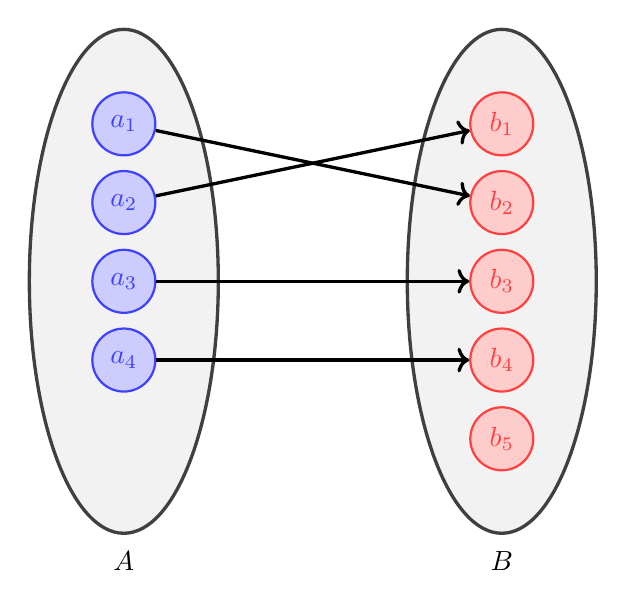
\begin{tikzpicture}[scale=0.8]
        \tikzstyle{blue-node}=[color=blue!75,fill=blue!20,thick,circle, draw, minimum width=0.8cm]
        \tikzstyle{red-node}=[color=red!75,fill=red!20,thick,circle, draw, minimum width=0.8cm]
        \tikzstyle{parent}=[color=black!75,fill=black!5,very thick]
        \tikzstyle{mapsto}=[->,very thick]
        % set A
        \draw [parent] (-2,0) ellipse (1.5cm and 4cm);       
        \node [blue-node] at (-2,2.5) (a1) {$a_1$};        
        \node [blue-node] at (-2,1.25) (a2) {$a_2$};
        \node [blue-node] at (-2,0) (a3) {$a_3$};
        \node [blue-node] at (-2,-1.25) (a4) {$a_4$} (-2,-4.75) node[anchor=south,color=black] {$A$};
        % set B
        \draw [parent] (4,0) ellipse (1.5cm and 4cm);
        \node [red-node] at (4,2.5) (b1) {$b_1$};
        \node [red-node] at (4,1.25) (b2) {$b_2$};
        \node [red-node] at (4,0)(b3) {$b_3$};
        \node [red-node] at (4,-1.25) (b4) {$b_4$};
        \node [red-node] at (4,-2.5) (b5) {$b_5$} (4,-4.75) node[anchor=south,color=black] {$B$};
        % mapsto
        \draw [mapsto] (a1) -- (b2);
        \draw [mapsto] (a2) -- (b1);
        \draw [mapsto] (a3) -- (b3);
        \draw [mapsto] (a4) -- (b4);
    \end{tikzpicture}
    \caption{Example of an injective function}
    \label{sketch-injective-function}
\end{figure}

\begin{exm}\label{exm-surjective-function}
    Let $f:\mathbb{R}\rightarrow\mathbb{R},f(x)=2x+3$. Is this function surjective?
    \begin{flushleft}
        \textbf{Answer}: For any $y=f(x)\in\mathbb{R}$ there exists an $x=\frac{y-3}{2}$
        such that
        \begin{align*}
            f(x) &= 2\left(\frac{y-3}{2}\right)+3 \\
                 &= y - 3 + 3 \\
                 &= y
        \end{align*}
        This proves that the function $f(x)=2x+3$ is surjective since $\text{Im}(f)=\mathbb{R}$. 
        With respect to \pref{figure}{sketch-surjective-function} this means that 
        every value from the codomain is taken on \textit{at least} once.
    \end{flushleft}
    \begin{rem}
        The strategy for determining whether a function is 
        surjective or not boils down to solving the original function definition
        for $x$ and plugging in this expression in $f(x)$. If you can show that 
        $f(x)=y$ then you are done, if not then the function is not surjective.
    \end{rem}
\end{exm}

\begin{figure}[ht!]
    \centering
    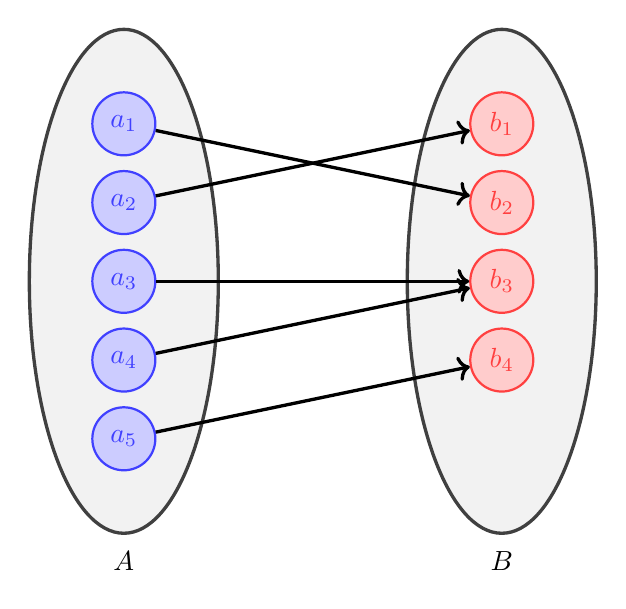
\begin{tikzpicture}[scale=0.8]
        \tikzstyle{blue-node}=[color=blue!75,fill=blue!20,thick,circle, draw, minimum width=0.8cm]
        \tikzstyle{red-node}=[color=red!75,fill=red!20,thick,circle, draw, minimum width=0.8cm]
        \tikzstyle{parent}=[color=black!75,fill=black!5,very thick]
        \tikzstyle{mapsto}=[->,very thick]
        % set A
        \draw [parent] (-2,0) ellipse (1.5cm and 4cm);       
        \node [blue-node] at (-2,2.5) (a1) {$a_1$};        
        \node [blue-node] at (-2,1.25) (a2) {$a_2$};
        \node [blue-node] at (-2,0) (a3) {$a_3$};
        \node [blue-node] at (-2,-1.25) (a4) {$a_4$};
        \node [blue-node] at (-2,-2.5) (a5) {$a_5$} (-2,-4.75) node[anchor=south,color=black] {$A$};
        % set B
        \draw [parent] (4,0) ellipse (1.5cm and 4cm);
        \node [red-node] at (4,2.5) (b1) {$b_1$};
        \node [red-node] at (4,1.25) (b2) {$b_2$};
        \node [red-node] at (4,0)(b3) {$b_3$};
        \node [red-node] at (4,-1.25) (b4) {$b_4$} (4,-4.75) node[anchor=south,color=black] {$B$};
        % mapsto
        \draw [mapsto] (a1) -- (b2);
        \draw [mapsto] (a2) -- (b1);
        \draw [mapsto] (a3) -- (b3);
        \draw [mapsto] (a4) -- (b3);
        \draw [mapsto] (a5) -- (b4);
    \end{tikzpicture}
    \caption{Example of an surjective function}
    \label{sketch-surjective-function}
\end{figure}

\begin{exm}\label{exm-bijective-function}
    Let $f:\mathbb{R}\rightarrow\mathbb{R},f(x)=2x+3$. Is this function bijective?
    \begin{flushleft}
        \textbf{Answer}: From \pref{example}{exm-injective-function} and
        \pref{example}{exm-surjective-function} we can deduce that since the function
        is injective and surjective, that it is bijective as well. With respect 
        to \pref{figure}{sketch-bijective-function} this means that every value 
        from the codomain is taken on \textit{exactly} once.
    \end{flushleft}
\end{exm}

\begin{figure}[ht!]
    \centering
    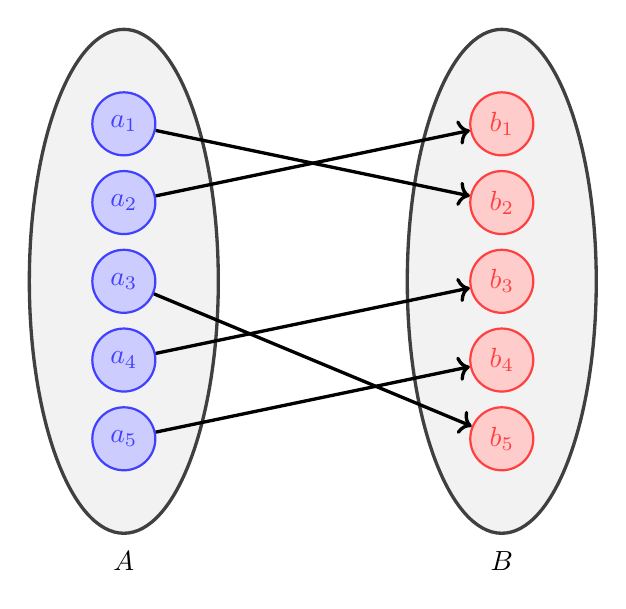
\begin{tikzpicture}[scale=0.8]
        \tikzstyle{blue-node}=[color=blue!75,fill=blue!20,thick,circle, draw, minimum width=0.8cm]
        \tikzstyle{red-node}=[color=red!75,fill=red!20,thick,circle, draw, minimum width=0.8cm]
        \tikzstyle{parent}=[color=black!75,fill=black!5,very thick]
        \tikzstyle{mapsto}=[->,very thick]
        % set A
        \draw [parent] (-2,0) ellipse (1.5cm and 4cm);       
        \node [blue-node] at (-2,2.5) (a1) {$a_1$};        
        \node [blue-node] at (-2,1.25) (a2) {$a_2$};
        \node [blue-node] at (-2,0) (a3) {$a_3$};
        \node [blue-node] at (-2,-1.25) (a4) {$a_4$};
        \node [blue-node] at (-2,-2.5) (a5) {$a_5$} (-2,-4.75) node[anchor=south,color=black] {$A$};
        % set B
        \draw [parent] (4,0) ellipse (1.5cm and 4cm);
        \node [red-node] at (4,2.5) (b1) {$b_1$};
        \node [red-node] at (4,1.25) (b2) {$b_2$};
        \node [red-node] at (4,0)(b3) {$b_3$};
        \node [red-node] at (4,-1.25) (b4) {$b_4$};
        \node [red-node] at (4,-2.5) (b5) {$b_5$} (4,-4.75) node[anchor=south,color=black] {$B$};
        % mapsto
        \draw [mapsto] (a1) -- (b2);
        \draw [mapsto] (a2) -- (b1);
        \draw [mapsto] (a3) -- (b5);
        \draw [mapsto] (a4) -- (b3);
        \draw [mapsto] (a5) -- (b4);
    \end{tikzpicture}
    \caption{Example of an bijective function}
    \label{sketch-bijective-function}
\end{figure}

\begin{exm}\label{exm-injective-surjective-bijective}
    Determine whether the following functions are injective, surjective or
    bijective\footnote{You may also consult \pref{figure}{sktech:exm-1:4} for
    additional help.}:
    \begin{enumerate}
        \item[1.)] $f(x):\mathbb{R}^+\rightarrow\mathbb{R}^+,x\mapsto x^2-1$
        \item[2.)] $g(x):\mathbb{R}^+\rightarrow\mathbb{R},x\mapsto x^2-1$
        \item[3.)] $h(x):\mathbb{R}\rightarrow\mathbb{R}^+,x\mapsto x^2-1$
        \item[4.)] $i(x):\mathbb{R}\rightarrow\mathbb{R},x\mapsto x^2-1$ 
    \end{enumerate}
    \begin{flushleft}
        \textbf{Answer:} TODO
    \end{flushleft}
\end{exm}

\begin{definition}\label{def-inverse-function}
    Let $f:\mathcal{D}\to\mathcal{C}$. We say that $f$ is invertible if there exists
    $f^{-1}:\mathcal{C}\to\mathcal{D}$ such that
    \begin{equation}
        \forall x\in\mathcal{D}:(f^{-1}\circ f)(x)=x 
        \land \forall y\in\mathcal{C}:(f \circ f^{-1})(y)=y
    \end{equation}
    If that's the case, we call $f^{-1}$ the inverse function of $f$.
\end{definition}

\begin{thm}\label{thm-inverse-function}
    A function $f$ is invertible, \textit{iff} it is bijective.
\end{thm}

\begin{rem}\label{rem-sqrt-function}
    In school we learnt that the function 
    \begin{equation}\label{eq-sqrt-function}
        f:\mathbb{R}^+\to\mathbb{R}^+,x\mapsto\sqrt{x}
    \end{equation}
    is the inverse function of
    \begin{equation}\label{eq-pow-function}
        f:\mathbb{R}\to\mathbb{R}^+,x\mapsto x^2
    \end{equation}
    Notice that the square root function in \pref{equation}{eq-sqrt-function} is 
    only defined for positive values on $\mathbb{R}$. This is because the principal
    square root is positive:
    \begin{equation}\label{eq-sqrt-abs-function}
        \sqrt{x^2}=\abs{x}
    \end{equation}
    You may have been taught in physics that the square root function can take on
    two values, \textit{i.e.} $\sqrt{x^2}=\pm x$, for example
    \begin{equation*}
        f(x=9)=\sqrt{9}\implies x=3 \lor x=-3
    \end{equation*}
    But \pref{theorem}{thm-inverse-function} states that inverse functions are 
    bijective\footnote{To satisfy this old notion, the square root function would
    have to be strictly surjective, see also \pref{figure}{sketch-surjective-function}.}.
    \begin{figure}[h!]
        \centering
        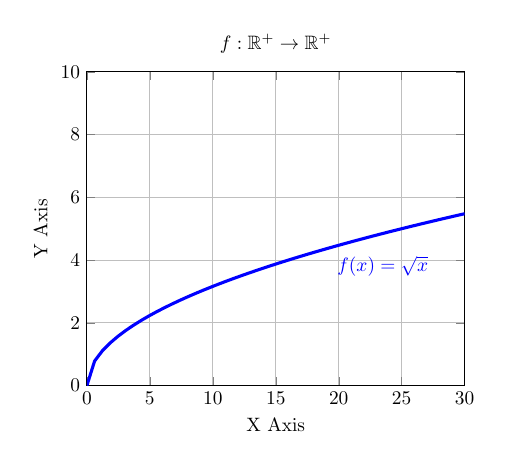
\begin{tikzpicture}[scale=0.7]
            \begin{axis}[
                xmax=30,
                xmin=0,
                ymax=10,
                ymin=0,
                samples=50,
                grid=major,
                xlabel={X Axis},
                ylabel={Y Axis},
                title={$f:\mathbb{R}^+\to\mathbb{R}^+$}
            ]
            \addplot[blue, ultra thick,domain=0:30]{sqrt(x)} node[anchor=north west,pos=0.65] {$f(x)=\sqrt{x}$};
        \end{axis}
        \end{tikzpicture}
        \caption{The square root function only operates with positive numbers}
        \label{sketch:rem-sqrt-function}
    \end{figure}
    So, while it is sometimes convenient to follow the convention in \pref{equation}{eq-sqrt-abs-function},
    strictly speaking the square root function only ever takes on positive values
    (\textit{cf.} \pref{figure}{sketch:rem-sqrt-function}).
\end{rem}

\begin{definition}\label{def-floor-function}
    The floor function is defined by
    \begin{equation}
        \ffloor(x)=\floor{x}\defines\max\left\{m\in\mathbb{Z}\setbuild m\leq x\right\}
    \end{equation}
\end{definition}

\begin{definition}\label{def-ceiling-function}
    The ceiling function is defined by
    \begin{equation}
        \fceil(x)=\ceil{x}\defines\min\left\{n\in\mathbb{Z}\setbuild n\geq x\right\}
    \end{equation}
\end{definition}

\begin{definition}\label{def-dirichlet-function}
    The Dirichlet function is defined by
    \begin{equation}
        D(x)=\begin{cases}
            1\text{ if }x\in\mathbb{Q}\\
            0\text{ else }
        \end{cases}
    \end{equation}
\end{definition}

\begin{definition}\label{def-absolute-value-function}
    The absolute value function is defined by
    \begin{equation}
        \forall x\in\mathbb{R}: \abs{x}\defines\max\{x,-x\}=\begin{cases}
            x\text{ if } x \geq 0 \\
            -x \text{ else }
        \end{cases}
    \end{equation}
\end{definition}

\begin{thm}\label{thm-absolute-value-properties}
    Below are listed some of the properties related to the absolute value; for
    any $x\in\mathbb{R}$ the following holds:
    \begin{enumerate}
        \item $\abs{x} \geq 0$
        \item $\abs{x} \geq \pm x$
        \item $\abs{x} = \abs{-x}$
        \item $\abs{x} = 0 \iff x = 0$
        \item $\abs{xy} = \abs{x}\abs{y}$
        \item $\abs{x} + \abs{y} \geq \abs{x+y}$
        \item $\abs{x-y} \geq \abs[\big]{\abs{x}-\abs{y}}$
        \item $\abs{x} < M \iff -M < x < M$
    \end{enumerate}
\end{thm}

\begin{proof}
    Of theorem (\ref{thm-absolute-value-properties}).
    \begin{flushleft}
        In this proof we will only show property 6 of this theorem which is also
        known as the triangle inequality. From property 2 it follows that the sum 
        of $\abs{x}\geq x$ and $\abs{y}\geq y$ equals
        \begin{equation}\label{tmp-absolute-value-properties:1}
            \abs{x} + \abs{y} \geq x + y
        \end{equation}
        Likewise, from $\abs{x}\geq -x$ and $\abs{y}\geq -y$ it follows that
        \begin{equation}\label{tmp-absolute-value-properties:2}
            \abs{x} + \abs{y} \geq -(x+y)
        \end{equation}
        Thus, by definition (\ref{def-absolute-value-function}) and equation
        (\ref{tmp-absolute-value-properties:1}) and (\ref{tmp-absolute-value-properties:2})
        we can conclude that
        \begin{equation*}
            \abs{x} + \abs{y} \geq \abs{x+y}
        \end{equation*}
    \end{flushleft}
\end{proof}

\begin{rem}
    A geometric interpretation of the absolute value function $\abs{x}$ is the 
    distance from $x$ to $0$. Similarly, the absolute value of the difference 
    $\abs{x-y}$ can be interpreted as the distance between $x$ and $y$. See also
    \hyperref[subsec-metric-spaces]{the subsection for metric spaces} for more 
    more information on distances.
\end{rem}


\subsection{Limit Prerequisites}\label{subsec-limit-prerequisites}

\begin{definition}\label{def-interval-notation}
    As opposed to closed intervals, open and half-open intervals contain infinitely
    many elements. The $\infty$ symbol always needs to be paired with a parenthesis
    rather than a bracket because it is technically incorrect to think of infinity
    as a number. So far, we haven't agreed on a formal definition for the concept
    of infinity, but it will become important later when we discuss limits in more
    detail.
    \begin{enumerate}
        \item $(a,b)\defines\left\{x\setbuild a < x < b\right\}       \quad \text{(Open interval)}$
        \item $(a,b]\defines\left\{x\setbuild a < x \leq b\right\}    \quad \text{(Half-open interval)}$
        \item $[a,b)\defines\left\{x\setbuild a \leq x < b\right\}    \quad \text{(Half-closed interval)}$
        \item $[a,b]\defines\left\{x\setbuild a \leq x \leq b\right\} \quad \text{(Closed interval)}$
    \end{enumerate}
\end{definition}

\begin{definition}\label{def-epsilon-neighborhood}
    Let $a\in\mathbb{R}$ and $\varepsilon > 0$. Then the open interval 
    $(a-\varepsilon,a+\varepsilon)$ is called the epsilon neighborhood of $a$
    and is denoted by
    \begin{equation}
        \mathcal{U}_\varepsilon(a)\defines
        \left\{x \setbuild x\in\mathbb{R},\abs{x-a}<\varepsilon \right\}=
        (a-\varepsilon,a+\varepsilon)
    \end{equation}
\end{definition}

\begin{rem}\label{rem-epsilon-neighborhood}
    In reference to property 8 of theorem (\ref{thm-absolute-value-properties})
    we can note that
    \begin{equation}
        x\in(a-\varepsilon,a+\varepsilon) \iff \abs{x-a} < \varepsilon
    \end{equation}
\end{rem}

\begin{definition}\label{def-epsilon-punctured-neighborhood}
    Let $a\in\mathbb{R}$. For $\varepsilon>0$ we define the punctured epsilon 
    neighborhood of $a$, denoted by 
    \begin{equation}
        \mathcal{U}_{\varepsilon}^{\bolddot}(a)\defines
        \left\{x \setbuild x\in\mathbb{R}, 0<\abs{x-a}<\varepsilon\right\}=
        (a-\varepsilon,a+\varepsilon)\setminus\{a\}
    \end{equation}
\end{definition}

\begin{definition}\label{def-limit-point}
    Let $M\subset\mathbb{R}$ and $a\in\mathbb{R}$. Then, $a$ is called a limit 
    point\footnote{Or cluster point} of $M$ \textit{iff}
    \begin{equation}
        \bigwedge_{\varepsilon>0}(M\cap\mathcal{U}_\varepsilon^{\bolddot}\neq\emptyset)
    \end{equation}
\end{definition}

\begin{definition}\label{def-isolated-point}
    In contrast to definition (\ref{def-limit-point}), we call $a$ an isolated point
    of $M$ \textit{iff}
    \begin{equation}
        \neg\bigwedge_{\varepsilon>0}(M\cap\mathcal{U}_\varepsilon^{\bolddot}\neq\emptyset)
        \iff
        \bigvee_{\varepsilon>0}(M\cap\mathcal{U}_\varepsilon^{\bolddot}=\emptyset)
    \end{equation}
    \textit{i.e.} $a\in M\subset\mathbb{R}$ and $a$ is not a limit point.
\end{definition}

\begin{rem}
    If $a$ is an isolated point of $M$, then \cite[p.67]{wuest2009}
    \begin{align*}
        a\in M:\mathcal{U}_\varepsilon(a)
        &=(\{a\}\cup\mathcal{U}_\varepsilon^{\bolddot})\cap M \\
        &=(\{a\}\cap M)\cup(\mathcal{U}_\varepsilon^{\bolddot}\cap M) \\
        &=\{a\}
    \end{align*}
    Therefore, in the neighborhood of $a$ are no other elements of the set $M$.
\end{rem}

\begin{exm}\label{exm-limit-points}
    Find the set of all limit points for
    \begin{enumerate}
        \item $A\defines\displaystyle\bigcup_{n\in\mathbb{N}}\left(\frac{1}{n},2-\frac{1}{n}\right)$
        \item $B\defines\left\{x\in\mathbb{R}\setbuild x=n+\frac{1}{m}\quad\text{($n,m$ appropriate)}\right\}$
    \end{enumerate}
    \begin{flushleft}
        \textbf{\nth{1} Answer:} TODO
    \end{flushleft}
    \begin{flushleft}
        \textbf{\nth{2} Answer:} TODO
    \end{flushleft}
\end{exm}

\begin{definition}\label{def-bounded-sets}
    Let $A \subseteq\mathbb{R}$ be a set.
    \begin{enumerate}
        \item Then $A$ is called bounded from above if there exists $M\in\mathbb{R}$ 
        such that $x\leq M$ for any $x\in A$.
        \item Similarly, $A$ is bounded from below if there exists $m\in\mathbb{R}$ 
        such that $x\geq M$ for any $x\in A$.
        \item Finally, $A$ is called bounded if it is bounded from above and below.
        \footnote{Notice that the boundary points in this definition
        lay no claim to uniqueness.}
    \end{enumerate}
\end{definition}

\begin{exm}\label{exm-bounded-sets:1}
    \hfill
    \begin{enumerate}
        \item Consider the set of natural numbers: $\mathbb{N}$ is not bounded from above, but 
        below, \textit{i.e.} $1$ is a lower bound of $\mathbb{N}$.
        \item Let $A=(-3,2]$. Then this set is bounded from above and below.
        \item Let $B=\left\{\frac{1}{n}\setbuild n\in\mathbb{N}\right\}$. Then this
        set is bounded from above by $1$, and bounded from below by $0$.
    \end{enumerate}
\end{exm}

\begin{definition}\label{def-supremum-infimum-sets}
    Let $A\subset\mathbb{R}$ be a set.
    \begin{enumerate}
        \item $S$ is called the supremum of $A$ if it is the smallest upper bound 
        of $A$, and is denoted by $S=\sup(A)$.
        \item $I$ is called the infimum of $A$ if it is the largest lower bound 
        of $A$, and is denoted by $I=\inf(A)$.
    \end{enumerate}
\end{definition}

\begin{exm}\label{exm-bounded-sets:2}
    Consider the sets from \pref{example}{exm-bounded-sets:1}. Then\footnote{Remark:
    $\mathbb{N}\defines\{1,2,3,\dots\}$}
    \begin{enumerate}
        \item $\inf(\mathbb{N})=1$
        \item $\inf(A)=-3$ and $\sup(A)=2$
        \item $\inf(B)=0$ and $\sup(B)=1$
    \end{enumerate}
\end{exm}

\begin{definition}\label{def-maximum-minimum}
    Let $A\subset\mathbb{R}$ be a set.
    \begin{enumerate}
        \item If $S=\sup(A)$, then $S\in A$ is also a maximum of $A$ and is denoted by $S=\max(A)$.
        \item If $I=\inf(A)$, then $I\in A$ is also a minimum of $A$ and is denoted by $I=\min(A)$.
    \end{enumerate}
\end{definition}

\begin{exm}\label{exm-bounded-sets:3}
    Expanding on the results from example (\ref{exm-bounded-sets:2}), we note that
    \begin{enumerate}
        \item $\min(\mathbb{N})=1$
        \item $\min(A)=\text{\gls{dne}}$ and $\max(A)=2$
        \item $\min(B)=\text{\gls{dne}}$ and $\max(B)=1$
    \end{enumerate}
\end{exm}

\begin{definition}\label{def-monotonicity}
    Let $x,y\in\mathbb{R}$. A function is called
    \begin{enumerate}
        \item monotonically increasing, if for all $x,y$ it follows that
        \begin{equation}\label{eq-monotonically-increasing}
            x<y \implies f(x)\leq f(y)
        \end{equation}
        \item strictly monotonically increasing, if for all $x,y$ follows that
        \begin{equation}\label{eq-strictly-monotonically-increasing}
            x<y \implies f(x)<f(y)
        \end{equation}
        \item monotonically decreasing, if for all $x,y$ follows that
        \begin{equation}\label{eq-monotonically-decreasing}
            x<y \implies f(x)\geq f(y)
        \end{equation}
        \item strictly monotonically decreasing, if for all $x,y$ follows that
        \begin{equation}\label{eq-strictly-monotonically-decreasing}
            x<y \implies f(x)>f(y)
        \end{equation}
    \end{enumerate}
\end{definition}

\begin{exm}
    Let $f(x)=\sin(x)$.
    \begin{enumerate}
        \item Then $f$ is strictly increasing on $[-\tfrac{\pi}{2},\tfrac{\pi}{2}]$.
        \item Then $f$ is strictly decreasing on $[\tfrac{\pi}{2},\tfrac{3\pi}{2}]$.
    \end{enumerate}
\end{exm}

\begin{definition}\label{def-even-function}
    Let $f$ be a function. Then, $f$ is called an even function if
    \begin{equation}
        \forall x\in\domain{f}:f(x)=f(-x)
    \end{equation}
\end{definition}

\begin{exm}
    See the list below for some even functions:
    \begin{itemize}
        \item $x\mapsto\abs{x}$
        \item $x\mapsto x^2$
        \item $x\mapsto\cos(x)$
    \end{itemize}
\end{exm}

\begin{definition}\label{def-odd-function}
    Let $f$ be a function. Then, $f$ is called an odd function if
    \begin{equation}
        \forall x\in\domain{f}:f(x)=-f(-x)
    \end{equation}
\end{definition}

\begin{exm}
    See the list below for some odd functions:
    \begin{itemize}
        \item $x\mapsto x$
        \item $x\mapsto x^3$
        \item $x\mapsto\sin(x)$
    \end{itemize}
\end{exm}

\begin{definition}
    Let $f$ be a function. Then, $f$ is called a periodic function if
    \begin{equation}
        \forall x\in\domain{f}\,\exists T\in\mathbb{R}: f(x)=f(x+T)
    \end{equation}
\end{definition}

\begin{exm}
    See the list below for some periodic functions:
    \begin{itemize}
        \item $x\mapsto\sin(x)$
        \item $x\mapsto\cos(x)$
        \item $x\mapsto\tan(x)$
        \item \hyperref[def-dirichlet-function]{$x\mapsto D(x)$}
    \end{itemize}
\end{exm}

\begin{definition}\label{def-bounded-function}
    Let $f$ be a function. Then, $f$ is called\footnote{This definition extends 
    the notion of boundaries as defined in \pref{definition}{def-bounded-sets} to 
    functions.}
    \begin{enumerate}
        \item bounded from above if
        \begin{equation}
            \forall x\in\domain{f}\,\exists M\in\mathbb{R}:f(x)\leq M
        \end{equation}
        \item bounded from below if 
        \begin{equation}
            \forall x\in\domain{f}\,\exists m\in\mathbb{R}:f(x)\geq m
        \end{equation}
        \item bounded if $f$ is bounded from above and below.
    \end{enumerate}
\end{definition}

\begin{exm}
    The function $f:\mathcal{D}\to\mathbb{R}$ with
    \begin{itemize}
        \item $\domain{f}=\mathbb{R}^-:f(x)=x$ is bounded from above but not below
        \item $\domain{f}=\mathbb{R}:f(x)=x^2$ is bounded from below, but not above
        \item $\domain{f}=\mathbb{R}^+:f(x)=\sqrt{x}$ is bounded from below, but not above
        \item $\domain{f}=\mathbb{R}:f(x)=\sin(x)$ is bounded from above and below
        \item $\domain{f}=\mathbb{R}:f(x)=\ffloor(x)$ is neither bounded from above nor below
    \end{itemize}
\end{exm}

\begin{rem}\label{rem-bounded-function}
    A function $f$ is bounded \textit{iff}
    \begin{equation}
        \forall x\in\domain{f}\,\exists B\in\mathbb{R}:\abs{f(x)}\leq B
    \end{equation}
    since $\abs{f(x)}\leq B\iff -B\leq f(x) \leq B$ by the \nth{8} property from
    \pref{theorem}{thm-absolute-value-properties}.
\end{rem}

\begin{definition}\label{def-supremum-infimum-functions}
    Let $f$ be a function. Then we define
    \begin{enumerate}
        \item the supremum of a function by
        \begin{equation}
            \sup_{x\in\mathcal{D}}(f)\defines\sup\left\{f(x)\setbuild x\in\mathcal{D}\right\}
        \end{equation}
        \item the infimum of a function by
        \begin{equation}
            \inf_{x\in\mathcal{D}}(f)\defines\inf\left\{f(x)\setbuild x\in\mathcal{D}\right\}
        \end{equation}
    \end{enumerate}
\end{definition}

\begin{exm}
    Let $f(x)=\arctan(x)$. Then,
    \begin{itemize}
        \item the supremum of this function is
        \begin{equation}
            \sup(f)=\frac{\pi}{2}
        \end{equation}
        \item the infimum of this function is
        \begin{equation}
            \inf(f)=-\frac{\pi}{2}
        \end{equation}
    \end{itemize}
\end{exm}

\begin{definition}\label{def-function-operations}
    Let $f$ and $g$ be two functions. Then we define
    \begin{enumerate}
        \item the addition between two functions by
        \begin{equation}
            (f \pm g)(x) \defines f(x) \pm g(x)
        \end{equation}
        \item the multiplication between two functions by
        \begin{equation}
            (f \cdot g)(x) \defines f(x) \cdot g(x)
        \end{equation}
        \item the division between two functions by\footnote{For $g(x)\neq0$}
        \begin{equation}
            \left(\frac{f}{g}\right)(x) \defines \frac{f(x)}{g(x)} 
        \end{equation}
        \item the composition between two functions by
        \begin{equation}
            (f \circ g)(x) \defines f(g(x))
        \end{equation}
    \end{enumerate}
\end{definition}

\begin{exm}
    Let $f:\mathbb{R}\to[-1,1],x\mapsto\sin(x)$ and $g:\mathbb{R}\setminus\{0\}\to\mathbb{R},x\mapsto\tfrac{1}{x}$.
    Then the two compositions for these functions are given by
    \begin{align*}
        &(f \circ g):\mathbb{R}\setminus\{0\}\to[-1,1],x\mapsto\sin\left(\frac{1}{x}\right)\\
        &(g \circ f):\mathbb{R}\setminus\left\{\pi k\setbuild k\in\mathbb{Z}\right\}\to\mathbb{R},x\mapsto\frac{1}{\sin(x)}
    \end{align*}
\end{exm}

\begin{rem}\label{rem-monotone-implies-injective}
    If $f$ is strictly monotone, then $f$ is injective.
\end{rem}

\begin{rem}\label{rem-elementary-functions}
    It is advised to remember the following elementary functions by heart:
    \begin{itemize}
        \item Polynomial functions\footnote{$a_0$ is the so-called \enquote{free coefficient}}: $p(x)=\sum_{i=0}^na_ix^i$
        \item Rational functions: $f(x)=\tfrac{p(x)}{q(x)}$ where $p(x)$ and $q(x)$ are well-defined polynomial functions
        \item Exponential functions: $f(x)=a^x$ for $a>0$ and $a\neq 1$
        \item Trigonometric functions: for example, $f(x)=\sin(x)$
        \item Inverse trigonometric functions: for example, $f^{-1}(x)=\arcsin(x)$
        \item Inverse functions of polynomials, for example $f^{-1}(x)=\sqrt{x}$
        \item Inverse functions of rationals
        \item Inverse functions of exponentials: for example, $f^{-1}(x)=\log_a(x)$
    \end{itemize}
\end{rem}

\begin{definition}\label{def-elementary-functions}
    An elementary function is any function obtained from the list in \pref{remark}{rem-elementary-functions},
    including their combinations using the operations defined in \pref{definition}{def-function-operations}.
    \footnote{Note that this is not a standard definition.}
\end{definition}


\subsection{Limits}\label{subsec-limits}

\begin{definition}\label{def-epsilon-delta-definition-limit}
	Let $f(x)$ be a function with $a,b\in\mathbb{R}$ with $a$ as a limit point of $\domain{f}$.
	Then the the function $f$ has the limit $b$ as $x$ approaches $a$, \textit{i.e.}
	\begin{equation}
		\bigwedge_{\varepsilon>0}\bigvee_{\delta>0}\bigwedge_{x\in\domain{f}}
		\left(0<\abs{x-a}<\delta\implies\abs{f(x)-b}<\varepsilon\right)
	\end{equation}
	The limit of this function is denoted by
	\begin{equation}
		\lim_{x\to a}f(x)=b,
	\end{equation}
\end{definition}

\begin{rem}
	The equation $\displaystyle\lim_{x\to a}f(x)=b$ is equivalent to the following
	expressions:
	\begin{enumerate}
		\item For $f$ there exists a limit (point) at $a$.
		\item This limit of $f$ is equal to $b$.
	\end{enumerate}
	In other words, $f$ has a limit at $a$ if
	\begin{equation*}
		\bigvee_{b\in\mathbb{R}}\bigwedge_{\varepsilon>0}\bigvee_{\delta>0}\bigwedge_{x\in\domain{f}}
		\left(0<\abs{x-a}<\delta \implies \abs{f(x)-b}<\varepsilon\right)
	\end{equation*}
\end{rem}

\begin{exm}\label{exm-epsilon-delta-definition-limit:1}
	Show that
	\begin{equation*}
		\lim_{x\to3}\frac{x-1}{2}=1
	\end{equation*}
	by using the epsilon-delta definition for limits.
	\begin{flushleft}
		\textbf{Answer}: Let $\varepsilon>0$ and $b\in\mathbb{R}$. Take
		$\delta\defines2\varepsilon$; Then $\abs{x-3}<\delta$, which implies
		\begin{align*}
			\abs{f(x)-b} & =\abs[\Bigg]{\frac{x-1}{2}-1} \\
			             & =\frac{\abs{x-3}}{2}          \\
			             & <\frac{\delta}{2}             \\
			             & =\varepsilon
		\end{align*}
	\end{flushleft}
\end{exm}

\begin{exm}\label{exm-epsilon-delta-definition-limit:2}
	Show that for some $a\in\mathbb{R}$,
	\begin{equation*}
		\lim_{x\to a}\sin(x)=\sin(a)
	\end{equation*}
	by using the epsilon-delta definition for limits.
	\begin{flushleft}
		\textbf{Answer}: Let $\varepsilon>0$ and $b\in\mathbb{R}$. Take
		$\varepsilon\defines\delta$ such that $\abs{x-a}<\delta$. Further, recall that
		\begin{align*}
			 & \text{(A)}:\forall\alpha\in\mathbb{R}:\abs{\cos(\alpha)}\leq1            \\
			 & \text{(B)}:\forall\alpha\in\mathbb{R}:\abs{\sin(\alpha)}\leq\abs{\alpha}
		\end{align*}
		\begin{align*}
			\abs{f(x)-b} & =\abs{\sin(x)-\sin(a)}                                                                                                    \\
			             & =\abs[\Bigg]{2\sin\left(\frac{x-a}{2}\right)\cos\left(\frac{x+a}{2}\right)}                                               \\
			             & =2\cdot\abs[\Bigg]{\sin\left(\frac{x-a}{2}\right)}\abs[\Bigg]{\cos\left(\frac{x+a}{2}\right)}                             \\
			             & \leq 2\cdot\frac{\abs{x-a}}{2}                                                                &  & \text{note (A) \& (B)} \\
			             & =\varepsilon
		\end{align*}
	\end{flushleft}
\end{exm}

\begin{exm}\label{exm-epsilon-delta-definition-limit:3}
	Show \cite[p.69]{wuest2009} that the function $f(x)=\tfrac{x^2-3x+2}{x(x-1)}$
	with $x\in\mathbb{R}\setminus\{0,1\}$ has the limit $b=-1$ as $x\to1$.
	\begin{flushleft}
		\textbf{Answer}: Let $\varepsilon>0$.
		\begin{align}
			\abs{f(x)-(-1)} & =\abs[\Bigg]{\frac{x^2-3x+2}{x(x-1)}+1}\nonumber                             \\
			                & =\abs[\Bigg]{\frac{(x-2)(x-1)}{x(x-1)}+1}\nonumber                           \\
			                & =\abs[\Bigg]{\frac{x-2}{x}+1}\nonumber                                       \\
			                & =\abs[\Bigg]{\frac{2x-2}{x}}\nonumber                                        \\
			                & =\frac{2}{\abs{x}}\cdot\abs{x-1}\label{eq3-epsilon-delta-definition-limit:1}
		\end{align}
		Since we aim for the neighborhood of $x=1$ we can impose the following
		restriction on this inequality:
		\begin{equation}\label{eq3-epsilon-delta-definition-limit:2}
			0<\abs{x-1}<\frac{1}{2}
		\end{equation}
		This in turn implies
		\begin{align}
			\abs{x} & =\abs{x-1+1}\nonumber                                                                                                               \\
			        & \geq1-\abs{x-1}\nonumber                                                                                                            \\
			        & >1-\frac{1}{2}                                           &  & \text{\pref{equation}{eq3-epsilon-delta-definition-limit:2}}\nonumber \\
			        & =\frac{1}{2}\label{eq3-epsilon-delta-definition-limit:3}
		\end{align}
		Hence,
		\begin{align}
			\abs{f(x)-b} & =\frac{2}{\abs{x}}\cdot\abs{x-1}                             &  & \text{\pref{equation}{eq3-epsilon-delta-definition-limit:1}}\nonumber \\
			             & <\frac{2}{\tfrac{1}{2}}\cdot\abs{x-1}                        &  & \text{\pref{equation}{eq3-epsilon-delta-definition-limit:3}}\nonumber \\
			             & =4\cdot\abs{x-1}\label{eq3-epsilon-delta-definition-limit:4}
		\end{align}
	\end{flushleft}
	Let $q(\varepsilon)\defines\min\left\{\tfrac{\varepsilon}{4},\tfrac{1}{2}\right\}$.
	Then for all $\varepsilon>0$ there exists a $\delta\defines q(\varepsilon)$ such that
	for $x\in\domain{f}$ it follows that
	\begin{align*}
		0<\abs{x-1}<\delta \implies \abs{f(x)-(-1)} & <4\cdot\abs{x-1}             &  & \text{\pref{equation}{eq3-epsilon-delta-definition-limit:4}} \\
		                                            & <4\cdot\frac{\varepsilon}{4}                                                                   \\
		                                            & =\varepsilon
	\end{align*}
\end{exm}

\begin{exm}\label{exm-epsilon-delta-definition-limit:4}
	Show that the function $f(x)=\tfrac{x^2-4x+3}{2x-6}$ with $x\in\mathbb{R}\setminus\{3\}$
	has the limit $b=1$ as $x\to3$.
	\begin{flushleft}
		\textbf{Answer}: Let $\varepsilon>0$. Define $\delta\defines2\varepsilon$,
		such that $\abs{x-3}<\delta$, wherefore
		\begin{align*}
			\abs{f(x)-b} & =\abs[\Bigg]{\frac{x^2-4x+3}{2x-6}-1}     \\
			             & =\abs[\Bigg]{\frac{(x-1)(x-3)}{2(x-3)}-1} \\
			             & =\abs[\Bigg]{\frac{1}{2}(x-1)-1}          \\
			             & =\abs[\Bigg]{\frac{1}{2}x-\frac{3}{2}}    \\
			             & =\frac{1}{2}\abs{x-3}                     \\
			             & <\frac{1}{2}\cdot2\varepsilon             \\
			             & =\varepsilon
		\end{align*}
	\end{flushleft}
\end{exm}

\begin{exm}\label{exm-epsilon-delta-definition-limit:5}
	Show that for $a>0$ ($a\in\mathbb{R}$),
	\begin{equation*}
		\sqrt{x}\tolim{x}{a}\sqrt{a}
	\end{equation*}
	\begin{flushleft}
		\textbf{Answer}: Let $\varepsilon>0$. When we define $\delta\defines\min\left\{a,\varepsilon\sqrt{a}\right\}$,
		then $\abs{x-a}<\delta$ implies that
		\begin{align*}
			\abs{f(x)-b} & =\abs[\big]{\sqrt{x}-\sqrt{a}}                                                         \\
			             & =\frac{\abs[\big]{\sqrt{x}-\sqrt{a}}\left(\sqrt{x}+\sqrt{a}\right)}{\sqrt{x}+\sqrt{a}} \\
			             & =\frac{\abs{x-a}}{\sqrt{x}+\sqrt{a}}                                                   \\
			             & <\frac{\abs{x-a}}{\sqrt{a}}                                                            \\
			             & <\frac{\varepsilon\sqrt{a}}{\sqrt{a}}                                                  \\
			             & =\varepsilon
		\end{align*}
		Therefore,
		\begin{equation*}
			\lim_{x\to a}\sqrt{x}=\sqrt{a}
		\end{equation*}
	\end{flushleft}
\end{exm}

\begin{rem}\label{rem-undefined-limits}
	Examples of functions where \pref{definition}{def-epsilon-delta-definition-limit} breaks:
	\begin{enumerate}
		\item For any $a\in\mathbb{Z}$, the limit of $f(x)=\floor{x}$ does not exists.
		\item The limit $\displaystyle\lim_{x\to0}\tfrac{1}{x}$ does not exists.
		\item The limit $\displaystyle\lim_{x\to0}\tfrac{1}{x^2}$ does not exists.
		\item The limit $\displaystyle\lim_{x\to0}\sin\left(\tfrac{1}{x}\right)$ does not exists.
	\end{enumerate}
\end{rem}

\begin{thm}\label{thm-limit-arithmetic}
	Let $\displaystyle\lim_{x \to a}f(x) = b_1$ and $\displaystyle\lim_{x \to a}g(x) = b_2$
	be two well-defined limits. Then the following statements hold:
	\begin{enumerate}
		\item $c \cdot f(x) \tolim{x}{a} c \cdot b_1 \quad (c\in\mathbb{R})$
		\item $f(x) + g(x) \tolim{x}{a} b_1 + b_2$
		\item $f(x) \cdot g(c) \tolim{x}{a} b_1 \cdot b_2$
		\item $\tfrac{f(x)}{g(x)} \tolim{x}{a} \tfrac{b_1}{b_2} \quad (b_2 \neq 0)$
	\end{enumerate}
\end{thm}


\begin{proof}
	Of \pref{theorem}{thm-limit-arithmetic}.
	\begin{flushleft}
		\textbf{\nth{2} Property}. From \pref{definition}{def-epsilon-delta-definition-limit}
		we can note that
		\begin{align*}
			 & \forall\varepsilon>0\;\exists\delta_1>0:\,\abs{x-a}<\delta_1\implies\abs{f(x)-b_1}<\frac{\varepsilon}{2} \\
			 & \forall\varepsilon>0\;\exists\delta_2>0:\,\abs{x-a}<\delta_2\implies\abs{g(x)-b_2}<\frac{\varepsilon}{2}
		\end{align*}
		Define $\delta\defines\min\{\delta_1,\delta_2\}$ Then, if $\abs{x-a}<\delta$,
		it follows from the triangle inequality that
		\begin{align*}
			\abs{f(x)+g(x)-(b_1+b_2)} & =\abs{(f(x)-b_1)+(g(x)-b_2)}                 \\
			                          & \leq\abs{f(x)-b_1}+\abs{g(x)-b_2}            \\
			                          & <\frac{\varepsilon}{2}+\frac{\varepsilon}{2} \\
			                          & =\varepsilon
		\end{align*}
	\end{flushleft}
\end{proof}

\begin{exm}
	Find the limit of
	\begin{equation*}
		\lim_{x \to 0}\left(\arctan\left(2\sqrt{\frac{\cos(x)}{3x+4}}\right)\right)=\frac{\pi}{4}
	\end{equation*}
	\begin{flushleft}
		\textbf{Answer}: TODO
	\end{flushleft}
\end{exm}

\begin{thm}\label{thm-absolute-value-of-limit:1}
	If $f(x) \tolim{x}{a} 0$, then this is equivalent to
	$\abs{f(x)} \tolim{x}{a} 0$.
\end{thm}

\begin{thm}\label{thm-absolute-value-of-limit:2}
	Let $b\in\mathbb{R}$. If $f(x) \tolim{x}{a} b$, then
	this implies $\abs{f(x)} \tolim{x}{a} \abs{b}$.
\end{thm}

\begin{rem}
	Note that the opposite direction of \pref{theorem}{thm-absolute-value-of-limit:2}
	is in general not true. A counter example for this would be the
	\hyperref[def-dirichlet-function]{Dirichlet function}.
\end{rem}

\begin{proof}
	Of \pref{theorem}{thm-absolute-value-of-limit:2}.
	\begin{flushleft}
		Let $\varepsilon>0$. Then $\abs{x-a}<\delta$ implies that
		\begin{align*}
			\abs[\big]{\abs{f(x) - \abs{b}}} & \leq \abs{f(x) - b} \\
			                                 & <\varepsilon
		\end{align*}
		by using the reverse triangle inequality for absolute values.
	\end{flushleft}
\end{proof}

\begin{thm}\label{thm-limit-monotonicity}
	Let $f(x) \geq g(x)$ for any $x\in\mathcal{U}_{\varepsilon}^{\bolddot}(a)$.
	If the limit of $f(x)$ and $g(x)$ exist, then
	\begin{equation*}
		\lim_{x \to a}f(x) \geq \lim_{x \to a}g(x)
	\end{equation*}
\end{thm}

\begin{rem}
	As for \pref{theorem}{thm-limit-monotonicity}, if $f(x) \geq 0$,
	then
	\begin{equation*}
		\lim_{x \to a}f(x) \geq 0
	\end{equation*}
\end{rem}

\begin{rem}
	\pref{Theorem}{thm-limit-monotonicity} does not hold if we replace the greater
	than or equal to inequality with a strictly greater than inequality.
\end{rem}

\begin{thm}\label{thm-unique-limit}
	If the limit of $\displaystyle\lim_{x\to a}f(x)=b\in\mathbb{R}$ exists, then $b$ is unique.
\end{thm}

\begin{proof}
	Of \pref{theorem}{thm-unique-limit}.
	\begin{flushleft}
		Assume \gls{wlog} that $b<c$ are both limits of this function. Define
		$\varepsilon\defines\tfrac{c-b}{3}>0$. Then by
		\pref{definition}{def-epsilon-delta-definition-limit} we have that
		\begin{equation}\label{eq-unique-limit:1}
			\exists\delta_1\text{ s.t. }a-\delta_1<x<a+\delta_1 \implies b-\varepsilon<f(x)<b+\varepsilon
		\end{equation}
		Likewise we know that
		\begin{equation}\label{eq-unique-limit:2}
			\exists\delta_2\text{ s.t. }a-\delta_1<x<a+\delta_1 \implies c-\varepsilon<f(x)<c+\varepsilon
		\end{equation}
	\end{flushleft}
	Therefore by \pref{equation}{eq-unique-limit:1} and \pref{equation}{eq-unique-limit:2},
	it follows that
	\begin{equation*}
		\left(f(x)<b+\varepsilon<c+\varepsilon\right)\land\left(c+\varepsilon<f(x)\right)
	\end{equation*}
	which is a contradiction.
\end{proof}

\begin{thm}\label{def-limit-is-bounded}
	If the limit of $\displaystyle\lim_{x\to a}f(x)=b\in\mathbb{R}$ exists, then
	$f$ is bounded in a neighborhood of $a$.
\end{thm}

\begin{thm}\label{thm-sandwich-theorem}
	Suppose that for any $x$ in a neighborhood of $a$
	\begin{equation*}
		h(x) \leq f(x) \leq g(x)
	\end{equation*}
	Further assume that
	\begin{equation*}
		\lim_{x \to a}h(x) = b = \lim_{x \to a}g(x)
	\end{equation*}
	Then it follows that
	\begin{equation*}
		\lim_{x \to a}f(x) = b
	\end{equation*}
\end{thm}

\begin{proof}
	Of \pref{theorem}{thm-sandwich-theorem}.
	\begin{flushleft}
		Let $\varepsilon>0$. Take $\delta\defines\min\{\delta_1,\delta_2\}$ where
		\begin{align*}
			 & 0 < \abs{x - a} < \delta_1 \implies \abs{g(x) - b} < \varepsilon \iff b - \varepsilon < g(x) < b + \varepsilon, \\
			 & 0 < \abs{x - a} < \delta_2 \implies \abs{h(x) - b} < \varepsilon \iff b - \varepsilon < h(x) < b + \varepsilon
		\end{align*}
		Therefore, if $0 < \abs{x - a} < \delta$,
		\begin{equation*}
			b - \varepsilon < h(x) \leq f(x) \leq g(x) < b + \varepsilon
		\end{equation*}
		which is equivalent to
		\begin{equation*}
			\abs{f(x) - b} < \varepsilon \iff \lim_{x \to a}f(x) = b
		\end{equation*}
	\end{flushleft}
\end{proof}

\begin{thm}\label{thm-product-of-bounded-zero-limit}
	If $\displaystyle\lim_{x \to a}f(x) = 0$ and $g(x)$ is bounded in a neighborhood
	of $a$, then
	\begin{equation*}
		\lim_{x \to a} \left(f(x)\cdot g(x)\right) = 0
	\end{equation*}
\end{thm}

\begin{proof}
	Of \pref{theorem}{thm-product-of-bounded-zero-limit}.
	\begin{flushleft}
		Since $g(x)$ is bounded, we can write $\abs{g(x)} \leq M$. So,
		\begin{align*}
			 & -M \leq \abs{g(x)} \leq M                                                                                                                                                                   \\
			\implies
			 & -M\cdot\abs{f(x)} \leq \abs{f(x)}\cdot\abs{g(x)} \leq M\cdot \abs{f(x)}                                                                                                                     \\
			\implies
			 & -M\cdot \lim_{x \to a}\abs{f(x)} \leq  \lim_{x \to a}\left(\abs{f(x)}\cdot\abs{g(x)}\right) \leq M \cdot \lim_{x \to a}\abs{f(x)}                                                           \\
			\implies
			 & -M \cdot 0 \leq \abs{f(x)}\cdot\abs{g(x)} \leq M \cdot 0                                                                          &  & \text{\pref{theorem}{thm-absolute-value-of-limit:1}} \\
			\implies
			 & 0 \leq \abs{f(x)}\cdot\abs{g(x)} \leq 0                                                                                           &  & \text{\pref{theorem}{thm-limit-arithmetic}}          \\
			\implies
			 & \lim_{x \to a}\left(\abs{f(x)}\cdot\abs{g(x)}\right)=0                                                                            &  & \text{\pref{theorem}{thm-sandwich-theorem}}          \\
			\implies
			 & \lim_{x \to a}\left(f(x)\cdot g(x)\right)=0                                                                                       &  & \text{\pref{theorem}{thm-absolute-value-of-limit:1}} \\
		\end{align*}
	\end{flushleft}
\end{proof}

\begin{exm}
	The limit of the function
	\begin{equation*}
		f(x) = x\cdot\sin\left(\frac{1}{x}\right)
	\end{equation*}
	as $x \to 0$ is
	\begin{equation*}
		\lim_{x \to 0}\left(x\cdot\sin\left(\frac{1}{x}\right)\right)=0
	\end{equation*}
	by \pref{theorem}{thm-product-of-bounded-zero-limit} since $\sin\left(\tfrac{1}{x}\right)$
	is bounded\footnote{But in and of itself not defined at $x=0$} by $[-1,1]$
	and the left factor of this function is $x=0$ as $x \to 0$.
\end{exm}

\begin{definition}\label{def-one-sided-limits}
	We denote the one-sided limit of the function $f(x)$ approached from the right by
	\begin{equation*}
		\lim_{x \to a^+}f(x)=b
	\end{equation*}
	if and only if
	\begin{equation}
		\forall\varepsilon>0\;\exists\delta>0:x\in(a,a+\delta)\implies\abs{f(x)-b}<\varepsilon
	\end{equation}
	Conversely, the left-sided limit is denoted by
	\begin{equation*}
		\lim_{x \to a^-}f(x)=b
	\end{equation*}
	if and only if
	\begin{equation}
		\forall\varepsilon>0\;\exists\delta>0:x\in(a-\delta,a)\implies\abs{f(x)-b}<\varepsilon
	\end{equation}
\end{definition}

\begin{rem}\label{rem-one-sided-limits}
	With respect to \pref{definition}{def-one-sided-limits}, note that there exist
	several equivalent notations. So, the right-sided limit of $f(x)$ can be denoted
	by
	\begin{equation*}
		\lim_{x \to a^+}f(x)=b
		\iff
		\lim_{x \underset{x>a}{\to} a}f(x)=b
		\iff
		\lim_{x\searrow  a}f(x)=b
	\end{equation*}
	Similarly, at times the left-sided limits may be denoted by
	\begin{equation*}
		\lim_{x \to a^-}f(x)=b
		\iff
		\lim_{x \underset{x<a}{\to} a}f(x)=b
		\iff
		\lim_{x \nearrow a}f(x)=b
	\end{equation*}
\end{rem}

\begin{thm}\label{thm-limit-exists-one-sided-limits}
	The limit of $f(x) \to b$ exists as $x \to a$ if and only if the left-sided
	limit as well as the right-sided limit of $f$ exists with
	\begin{equation}
		\lim_{x \to a}f(x)=b \iff \lim_{x \to a^+}f(x)=b=\lim_{x \to a^-}f(x)
	\end{equation}
\end{thm}

\begin{proof}
	Of \pref{theorem}{thm-limit-exists-one-sided-limits}.
	\begin{flushleft}
		TODO
	\end{flushleft}
\end{proof}

\begin{exm}\label{exm-important-sin-over-x-limit}
	Show that\footnote{This is a very useful limit that we are going to encounter
		more often in the near future.}
	\begin{equation}\label{eq-important-sin-over-x-limit}
		\lim_{x \to 0}\frac{\sin(x)}{x}=1
	\end{equation}
	\begin{flushleft}
		\textbf{Answer}: From figure (??) we can derive two observations:
		\begin{equation*}
			\forall x\in\left(0,\frac{\pi}{2}\right)\implies \sin(x)<x
		\end{equation*}
		Notice also that
		\begin{equation*}
			x < \tan(x)
		\end{equation*}
		So, this implies
		\begin{equation}\label{eq-important-sin-over-x-limit:1}
			\sin(x) < x < \tan(x)
		\end{equation}
		Furthermore, figure (??) reveals that
		\begin{equation*}
			\forall x\in\mathbb{R}:\abs{\sin(x)}\leq\abs{x}
		\end{equation*}
		From \pref{equation}{eq-important-sin-over-x-limit:1} follows that for all
		$\tfrac{\pi}{2}>x>0$:
		\begin{align*}
			\implies
			 & \frac{1}{\sin(x)} > \frac{1}{x} > \frac{1}{\tan(x)}                                                              \\
			\implies
			 & 1 > \frac{\sin(x)}{x} > \cos(x)                                                                                  \\
			\implies
			 & 1 > \lim_{x \to 0^+}\frac{\sin(x)}{x} > \lim_{x \to 0^+}\cos(x)                                                  \\
			\implies
			 & 1 > \lim_{x \to 0^+}\frac{\sin(x)}{x} > 1                                                                        \\
			\implies
			 & \lim_{x \to 0^+}\frac{\sin(x)}{x}=1                             &  & \text{theorem (\ref{thm-sandwich-theorem})}
		\end{align*}
		A similar argument can be made for
		\begin{align*}
			\forall x\in\left(-\frac{\pi}{2},0\right):\lim_{x \to 0^-}\frac{\sin(x)}{x}=1
		\end{align*}
		Last but not least, \pref{theorem}{thm-limit-exists-one-sided-limits} ensures
		that the limit in \pref{equation}{eq-important-sin-over-x-limit} exists.
	\end{flushleft}
\end{exm}

\begin{thm}\label{thm-monotone-one-sided-limits}
	Assume that $f$ is monotone on some interval $[a,b]$. Then $f$ has one-sided
	limits at every point.
\end{thm}

\begin{definition}\label{def-infinity-limits}
	Let $f$ be a function such that\footnote{In other words, $\infty$ is a limit
		point of the domain of $f$}
	\begin{equation}
		\forall c\in\mathbb{R}: (c,\infty)\cap\domain{f}\neq\emptyset
	\end{equation}
	Next let $b\in\mathbb{R}$. We say that $f(x) \to b$ for $x \to \infty$ if and only if
	\footnote{Similarly, we can define the limit for $f(x) \to b$ as $x \to -\infty$}
	\begin{equation}
		\bigwedge_{\varepsilon>0}\bigvee_{c\in\mathbb{R}}\bigwedge_{x\in\domain{f}}
		\left(x>c \implies \abs{f(x) - b}<\varepsilon\right)
	\end{equation}
	Then this is equivalent to \cite[p.70]{wuest2009}
	\begin{equation}
		\lim_{x \to \infty}f(x)=b
	\end{equation}
\end{definition}

\begin{rem}
	Definition (\ref{def-infinity-limits}) works with all previously encountered theorems.
\end{rem}

\begin{exm}\label{exm-infinity-limit:1}
	Let $f$ be defined by \cite[p.71]{wuest2009}
	\begin{equation*}
		f(x)\defines\frac{3x^2-2x+1}{x^2+5x}
	\end{equation*}
	where $x\in(0,\infty)$. Show that
	\begin{equation*}
		\lim_{x \to \infty}f(x)=3
	\end{equation*}
	\begin{flushleft}
		\textbf{Answer}: First observe, that for very large $x$ the quadratic terms
		in the numerator and denominator dominate over the other terms in the long
		run. Keeping this in mind we can make an intelligent guess for the limit point
		$f(x) \to 3$ as $x \to \infty$. Now for the formal part of this proof: Let $x>0$.
		Then, for $a(\varepsilon)\defines\max\left\{1,\tfrac{18}{\varepsilon}\right\}$ it
		follows that
		\begin{align*}
			\abs{f(x) - b} & = \abs[\Bigg]{\frac{3x^2-2x+1}{x^2+5x}-3}                               \\
			               & = \abs[\Bigg]{\frac{3x^2-2x+1-3x^2-15x}{x^2+5x}}                        \\
			               & = \abs[\Bigg]{\frac{-17x+1}{x^2+5x}}                                    \\
			               & \leq {\frac{\abs{-17x}+\abs{1}}{x^2+5x}}                                \\
			               & = \frac{17x}{x^2+5x} + \frac{1}{x^2+5x}                                 \\
			               & \leq \frac{17x}{x^2} + \frac{1}{x^2}                                    \\
			               & \leq \frac{18}{x}                                &  & \text{if } x\geq1 \\
			               & < \frac{18}{\tfrac{18}{\varepsilon}}                                    \\
			               & = \varepsilon
		\end{align*}
		in other words for every $\varepsilon>0$ there exists a $c\in\mathbb{R}$
		such that $c\defines a(\varepsilon)$ for which is true that
		\begin{equation*}
			x>c \implies \abs{f(x)-b}<\varepsilon
		\end{equation*}
		which means that $f(x)$ converges towards $3$ as $x$ approaches infinity.
	\end{flushleft}
\end{exm}

\begin{definition}\label{def-infinite-limits}
	We say a function has an infinite limit at infinity when
	\begin{equation}
		\bigwedge_{c\in\mathbb{R}}\bigvee_{\delta>0}
		\left(\abs{x-a}<\delta \implies f(x)>c\right)
	\end{equation}
	which is denoted by
	\begin{equation}
		\lim_{x \to a}f(x)=\infty
	\end{equation}
	Another frequently used expression to describes this behavior is divergence;
	limits that exhibit this type behavior are said to diverge.
\end{definition}

\begin{exm}\label{exm-infinity-limit:3}
	Use \pref{definition}{def-infinite-limits} to show that
	\begin{equation}
		\lim_{x \to 0}\frac{1}{x^2}=\infty
	\end{equation}
	\begin{flushleft}
		\textbf{Answer}: Let $c\in\mathbb{R}^+$ such that $\delta\defines\tfrac{1}{\sqrt{c}}$.
		Then, it follows that
		\begin{equation*}
			0<\abs{x-0}<\delta \implies \abs{x} < \frac{1}{\sqrt{c}} \implies \frac{1}{x^2} > c
		\end{equation*}
	\end{flushleft}
\end{exm}

\begin{rem}
	Beware: for $f(x) \to \pm\infty$ not all theorems hold, in particular
	\pref{theorem}{thm-limit-arithmetic} is only partially true.
\end{rem}

\begin{thm}\label{thm-pizza-theorem}
	If $g(x) \geq f(x)$ in a neighborhood of $a$ and $f(x) \to \infty$ as $x \to a$,
	then $g(x) \to \infty$ for $x \to a$.
\end{thm}


\subsection{Sequences}\label{subsec-sequences}

\begin{definition}\label{def-sequence}
	An infinite ordered set of real\footnote{This document restricts the definition
		to the set of real numbers, but in other courses it can be more abstract than that}
	numbers is called a sequence, most formally denoted by $\{a_n\}_{n=1}^\infty$,
	or just $a_n$.
\end{definition}

\begin{definition}\label{def-sequence-recursive:1}
	Let $a\in\mathbb{N}$. We define \cite[p.51]{wuest2009}
	\begin{align*}
		a_1     & = a + 1   \\
		a_{n+1} & = a_n + 1
	\end{align*}
\end{definition}

\begin{definition}\label{def-sequence-recursive:2}
	Let $a\in\mathbb{R}\setminus\{0\}$. We define \cite[p.51]{wuest2009}
	\begin{align*}
		a^0     & = 1                                                                         \\
		a^{n+1} & = a^n \cdot n &  & (n\in\mathbb{N}_0\defines\mathbb{N}\cup\{0\}=\mathbb{Z})
	\end{align*}
\end{definition}

\begin{definition}\label{def-sequence-recursive:3}
	Let $n\in\mathbb{N}_0$. We define \cite[p.51]{wuest2009}
	\begin{align*}
		0!     & = 1       \\
		(n+1)! & = n!(n+1)
	\end{align*}
	This is known as the faculty.
\end{definition}

\begin{definition}\label{def-sequence-recursive:4}
	Let $c\in\mathbb{Z}$ and $\{a_n\}_{n\in\mathbb{Z}_c}$ be sequences. We define \cite[p.51]{wuest2009}
	\begin{align*}
		\sum_{k=c}^n a_k     & = a_c                                                \\
		\sum_{k=c}^{n+1} a_k & = \sum_{k=c}^n a_k + a_{n+1} &  & (n\in\mathbb{Z}_c)
	\end{align*}
	This is known as the sum.
\end{definition}

\begin{definition}\label{def-sequence-recursive:5}
	Let $c\in\mathbb{Z}$ and $\{a_n\}_{n\in\mathbb{Z}_c}$ be sequences. We define \cite[p.51]{wuest2009}
	\begin{align*}
		\prod_{k=c}^n a_k     & = a_c                                                                  \\
		\prod_{k=c}^{n+1} a_k & = \left(\prod_{k=c}^n a_k\right) \cdot a_{n+1} &  & (n\in\mathbb{Z}_c)
	\end{align*}
	This is known as the product.
\end{definition}

\begin{rem}
	A sequence can also be written as a function $f:\mathbb{N}\to\mathbb{R}$,
	where $a_n = f(n)$.
\end{rem}

\begin{definition}\label{def-sequence-limit}
	Let $a_n$ be a sequence. We say that
	\begin{equation*}
		\lim_{n\to\infty}a_n=b
	\end{equation*}
	for $b\in\mathbb{R}$ if and only if
	\begin{equation*}
		\forall\varepsilon>0\;\exists N\in\mathbb{N}: n>N \implies \abs{a_n - b}<\varepsilon
	\end{equation*}
\end{definition}

\begin{rem}\label{rem-remarkable-sequences}
	What follows is a short list of some of the more notable sequences that we will
	get to know over time:
	\begin{enumerate}
		\item Linear sequence: $a_n=n$, \textit{e.g.} $1,3,4,5,\dots$
		\item Harmonic sequence: $a_n=\tfrac{1}{n}$, \textit{e.g.} $1,\tfrac{1}{2},\tfrac{1}{3},\tfrac{1}{4},\tfrac{1}{5},\dots$
		\item Alternating sequence: $a_n=(-1)^n$, \textit{e.g.} $-1,1,-1,1,-1,\dots$
		\item Alternating harmonic sequence: $a_n=\tfrac{(1)^{n}}{n}$, \textit{e.g.} $1,-\tfrac{1}{2},\tfrac{1}{3},-\tfrac{1}{4},\tfrac{1}{5},\dots$
		\item Arithmetic sequence: $a_n=5+2(n-1)$, \textit{e.g.} $5,7,9,11,13,\dots$
		\item Geometric sequence: $a_n=3\cdot2^{n-1}$, \textit{e.g.} $3,6,12,24,48,\dots$
		\item Constant sequence: $a_n=2$, \textit{e.g.} $2,2,2,2,2,\dots$
		\item Case sequence: $a_n=\begin{cases}1\text{ if }n\text{ is even}\\n\text{ else}\end{cases}$, \textit{e.g.} $1,1,3,1,5,\dots$
		\item Sequence of prime numbers\footnote{To date there exists no known formula for this sequence}, \textit{e.g.} $2,3,5,7,11,\dots$
		\item Sequence of digital digits of $\pi$, \textit{e.g.} $1,4,1,5,9,\dots$
		\item Recursive sequence: $a_n=\begin{cases}a_1=2\\a_n=3a_{n-1}^2\end{cases}$, \textit{e.g.} $2,12,432,559.872,\dots$
	\end{enumerate}
\end{rem}

\begin{exm}\label{exm-harmonic-sequence}
	Let $a_n$ be the harmonic sequence. Show that $\tfrac{1}{n}\to0$ as $n\to\infty$.
	\begin{flushleft}
		\textbf{Answer}: Let $\varepsilon>0$ and $N>\tfrac{1}{\varepsilon}$. Then,
		\begin{align*}
			\abs{f(x) - b} & = \abs[\Bigg]{\frac{1}{n}-0} \\
			               & = \frac{1}{n}                \\
			               & < \frac{1}{N}                \\
			               & < \varepsilon
		\end{align*}
	\end{flushleft}
\end{exm}

\begin{rem}
	Adding, dropping or changing any finite number of elements in a sequence does
	not affect the limit.
\end{rem}

\begin{thm}\label{thm-sequence-unique-limit}
	If $a_n$ has a limit, then the limit is unique.
\end{thm}

\begin{thm}\label{thm-sequence-limit-bounded}
	If $a_n$ has a limit, then $a_n$ is also bounded.
\end{thm}

\begin{rem}\label{rem-sequence-limit-bounded}
	\pref{Theorem}{thm-sequence-limit-bounded} only works in one direction; the
	limit might not exist if the sequence is bounded. Take for instance the alternating
	sequence as an counter example. Conversely, if the sequence is not bounded, then
	it has no finite limit.
\end{rem}

\begin{proof}
	Of \pref{theorem}{thm-sequence-limit-bounded}.
	\begin{flushleft}
		Suppose that $a_n$ has a limit, \textit{i.e.}
		\begin{equation*}
			\lim_{n\to\infty}a_n=b
		\end{equation*}
		then define
		\begin{equation*}
			M\defines\max\left\{b+1,a_1,a_2,\dots,a_N\right\}
		\end{equation*}
		for $n>N$ such that $a_n\in(b-1,b+1)$. We define
		\begin{equation*}
			m\defines\min\left\{b-1,a_1,a_2,\dots,a_N\right\}
		\end{equation*}
		Hence, $m \leq a_n \leq M$ for all $n\in\mathbb{N}$.
	\end{flushleft}
\end{proof}

\begin{thm}\label{thm-sequence-arithmetic}
	Let $a_n \seqinfty{n} L$ and $b_n \seqinfty{n} K$ be two limited sequences. Then
	\begin{enumerate}
		\item $\forall c\in\mathbb{R}:c \cdot a_n \seqinfty{n} c \cdot L$
		\item $a_n+b_n \seqinfty{n} L+K$
		\item $a_n \cdot b_n \seqinfty{n} L \cdot K$
		\item $\tfrac{a_n}{b_n} \seqinfty{n} \tfrac{L}{K}$ if $b_n \neq 0$ and $K \neq 0$
	\end{enumerate}
\end{thm}

\begin{exm}\label{exm-sequence-arithmetic:1}
	By \pref{example}{exm-harmonic-sequence} and \pref{theorem}{thm-sequence-arithmetic}
	it immediately follows that
	\begin{equation*}
		1+\frac{1}{n} \seqinfty{n} 1
	\end{equation*}
\end{exm}

\begin{thm}\label{thm-sequence-sqrt-limit}
	Let $a_n \seqinfty{n} b$. Assume that for any $a_n\geq0$ ($n\in\mathbb{N}$),
	\begin{equation*}
		\sqrt{a_n} \seqinfty{n} \sqrt{b}
	\end{equation*}
\end{thm}

\begin{thm}\label{thm-sequence-abs}
	Let $a_n \seqinfty{n} b$. Then
	\begin{equation*}
		\abs{a_n} \seqinfty{n} \abs{b}
	\end{equation*}
\end{thm}

\begin{thm}\label{thm-sequence-zero-limit}
	Let $a_n \seqinfty{n} 0$. Then this is equivalent to
	\begin{equation*}
		\abs{a_n} \seqinfty{n} 0
	\end{equation*}
\end{thm}

\begin{rem}\label{rem-sequence-abs}
	Note that for \pref{theorem}{thm-sequence-abs},
	\begin{equation*}
		\abs{a_n} \seqinfty{n} \abs{b} \notimplies a_n \seqinfty{n} b
	\end{equation*}
	The alternating sequence from \pref{remark}{rem-remarkable-sequences} is a
	counterexample for this statement.
\end{rem}

\begin{exm}\label{exm-sequence-arithmetic:2}
	Find the limit of
	\begin{equation*}
		\lim_{n\to\infty}\sqrt{\frac{n+1}{3n-\frac{2}{n}}}
	\end{equation*}
	\begin{flushleft}
		\textbf{Answer}: We use the result from \pref{example}{exm-harmonic-sequence},
		\textit{i.e.} $\tfrac{1}{n} \seqinfty{n} 0$ and some basic algebraic manipulation to get
		\begin{align*}
			\lim_{n\to\infty}\sqrt{\frac{n+1}{3n-\frac{2}{n}}}
			 & = \lim_{n\to\infty}\sqrt{\frac{1+\frac{1}{n}}{3-\frac{2}{n^2}}}                                                                                                                    \\
			 & = \lim_{n\to\infty}\sqrt{\frac{1+\frac{1}{n}}{3-2\cdot\frac{1}{n}\cdot\frac{1}{n}}}                                                                                                \\
			 & = \frac{1}{\sqrt{3}}                                                                &  & \text{\pref{theorem}{thm-sequence-arithmetic} \& \pref{theorem}{thm-sequence-zero-limit}}
		\end{align*}
	\end{flushleft}
\end{exm}

\begin{thm}\label{thm-product-of-bounded-zero-sequence}
	If $a_n \seqinfty{n} 0$ and $b_n$ is a bounded sequence, then\footnote{This is
		analogous to \pref{theorem}{thm-product-of-bounded-zero-limit}}
	\begin{equation*}
		a_n \cdot b_n \seqinfty{n} 0
	\end{equation*}
\end{thm}

\begin{thm}\label{thm-sequence-sandwich-theorem}
	Assume that
	\begin{equation*}
		a_n \leq b_n \leq c_n
	\end{equation*}
	as well as
	\begin{equation*}
		\lim_{n\to\infty} a_n = L = \lim_{n\to\infty} c_n
	\end{equation*}
	Then the sandwich theorem for sequences states that
	\begin{equation*}
		\lim_{n\to\infty} b_n = L
	\end{equation*}
\end{thm}

\begin{exm}
	Take the sequence $a_n=\tfrac{1}{n}\sin(n)$. We can find lower and upper bounds
	for this sequence since $\codomain{\sin(n)}=[-1,1]$, such that
	\begin{equation*}
		-\frac{1}{n}\leq\frac{\sin(n)}{n}\leq\frac{1}{n}
	\end{equation*}
	Notice that by \pref{theorem}{thm-sequence-zero-limit},
	\begin{equation*}
		\abs[\Bigg]{-\frac{1}{n}} \seqinfty{n} 0
	\end{equation*}
	Hence, by \pref{theorem}{thm-sequence-sandwich-theorem}
	\begin{equation*}
		\lim_{n\to\infty}\frac{\sin(n)}{n}=0
	\end{equation*}
\end{exm}

\begin{exm}
	Let $a_n=\tfrac{n!}{n^n}$. We claim that $a_n$ is bounded from above by the
	sequence $\tfrac{1}{n}$ since
	\begin{align*}
		\frac{n!}{n^n}                                                                           & \leq\frac{1}{n}                                         \\
		\iff
		n!n                                                                                      & \leq n^n                                                \\
		\iff
		n!                                                                                       & \leq n^{n-1}                                            \\
		\iff
		\underbrace{n \cdot (n-1) \cdot (n-2) \cdots 3 \cdot 2 \cdot 2 \cdot 1}_{n\text{ times}} & \leq \underbrace{n \cdot n \cdots n}_{n-1\text{ times}} \\
		\iff
		\underbrace{n \cdot (n-1) \cdot (n-2) \cdots 3 \cdot 2 \cdot 2}_{n-1\text{ times}}       & \leq \underbrace{n \cdot n \cdots n}_{n-1\text{ times}} \\
	\end{align*}
	The sequence is also bounded from below by $0$, so by theorem (\ref{thm-sequence-sandwich-theorem})
	it follows that
	\begin{equation*}
		0\leq\frac{n!}{n^n}\leq\frac{1}{n}\implies\lim_{n\to\infty}\frac{n!}{n^n}=0
	\end{equation*}
\end{exm}

\begin{thm}\label{thm-sequence-nth-root}
	Let $a_n=\sqrt[n]{n}$. Then this sequence converges to
	\begin{equation*}
		\sqrt[n]{n} \seqinfty{n} 1
	\end{equation*}
\end{thm}

\begin{thm}\label{thm-sequence-nth-root-of-constant}
	Let $a_n=\sqrt[n]{c}$ for any $c\in\mathbb{R}^+\setminus\{0\}$. Then this
	sequence converges to
	\begin{equation*}
		\sqrt[n]{c} \seqinfty{n} 1
	\end{equation*}
\end{thm}

\begin{exm}\label{exm-sequence-nth-root}
	Consider the sequence
	\begin{equation*}
		a_n =\sqrt[n]{3^{2n+1} \cdot n}
	\end{equation*}
	Then this is the same as
	\begin{equation*}
		a_n = \sqrt[n]{9^n}\sqrt[n]{3}\sqrt[n]{n} = 9\sqrt[n]{3}\sqrt[n]{n}
	\end{equation*}
	So, by \pref{theorem}{thm-sequence-nth-root} and \pref{theorem}{thm-sequence-nth-root-of-constant}
	this implies
	\begin{equation*}
		a_n \seqinfty{n} 9
	\end{equation*}
\end{exm}

\begin{thm}\label{thm-sequence-converges-positively}
	Let $a_n\geq0$. Then\footnote{This is still true if we only require $a_n\geq0$
		for some threshold $n\geq N\in\mathbb{N}$.},
	\begin{equation*}
		a_n \seqinfty{n} b \implies b \geq 0
	\end{equation*}
\end{thm}

\begin{thm}\label{thm-sequence-limit-greater-than}
	Suppose that $a_n \geq b_n$. Let $a_n \seqinfty{n} K$ and $b_n \seqinfty{n} L$. Then
	\footnote{This would be no longer true for strict inequalities, \textit{cf.} the
		sequence $0<\tfrac{1}{n}\seqinfty{n}0$.},
	\begin{equation*}
		K = \lim_{n\to\infty} a_n \geq \lim_{n\to\infty} b_n = L
	\end{equation*}
\end{thm}

\begin{thm}\label{thm-sequence-greater-than}
	If $a_n \seqinfty{n} L$ and $b_n \seqinfty{n} K$ with $L > K$, then there exists
	a threshold $n>N\in\mathbb{N}$ such that $a_n>b_n$.
\end{thm}

\begin{definition}\label{def-sequence-divergence}
	We say\footnote{Also called divergence of a sequence} that $a_n \seqinfty{n} \infty$
	if for every $M$ there exists an $N\in\mathbb{N}$ such that
	\begin{equation*}
		n>N \implies a_n > M
	\end{equation*}
\end{definition}

\begin{rem}
	Here are some sequences that diverge towards infinity:
	\begin{enumerate}
		\item $a_n=n!$
		\item $a_n=2^n$
		\item $a_n=n^3$
	\end{enumerate}
	Another very interesting sequence is $a_n=(-1)^n\cdot n$. It's an unbounded
	alternating sequence that bounces between $-\infty$ for odd numbers, and
	$+\infty$ for even numbers.
\end{rem}

\begin{thm}\label{thm-sequence-infinity-zero}
	If $a_n \seqinfty{n} \infty$, then $\tfrac{1}{a_n} \seqinfty{n} 0$.
\end{thm}

\begin{thm}\label{thm-sequence-zero-infinity}
	If $a_n>0$ for all $n\in\mathbb{N}$ where $a_n \seqinfty{n} 0$, then
	$\tfrac{1}{a_n} \seqinfty{n} \infty$.
\end{thm}

\begin{thm}
	If $a_n \geq b_n$ and $b_n \seqinfty{n} \infty$, then $a_n \seqinfty{n} \infty$.
\end{thm}

\begin{definition}\label{def-monotonicity-sequences}
	Let $a_n$ be a sequence. It is called
	\begin{enumerate}
		\item monotonically increasing, if $\forall n>N\in\mathbb{N}:a_{n+1} \geq a_n$
		\item strictly monotonically increasing, if $\forall n>N\in\mathbb{N}:a_{n+1} > a_n$
		\item monotonically decreasing, if $\forall n>N\in\mathbb{N}:a_{n+1} \leq a_n$
		\item strictly monotonically decreasing, if $\forall n>N\in\mathbb{N}:a_{n+1} < a_n$
	\end{enumerate}
\end{definition}

\begin{exm}\label{exm-monotonicity-sequences:1}
	We claim that $a_n=\tfrac{n^2}{2^n}$ is a monotonically decreasing sequence for $n>3$.
	\begin{flushleft}
		\textbf{Answer}: To prove this, we need to show that $a_{n+1}<a_n$. So,
		\begin{align*}
			\frac{a_{n+1}}{a_n} & = \frac{(n+1)^2}{2^{n+1}}\cdot\frac{2^n}{n^2}           \\
			                    & = \frac{1}{2}\left(\frac{n+1}{n}\right)^2               \\
			                    & = \frac{1}{2}\left(1+\frac{1}{n}\right)^2               \\
			                    & < 1                                           & (\star)
		\end{align*}
		The inequality in $(\star)$ holds \textit{iff} $n>3:\left(1+\tfrac{1}{n}\right)^2<2$.
		But then
		\begin{align*}
			\frac{1}{n}                  & \leq \frac{1}{3}                  \\
			\implies
			1+\frac{1}{n}                & \leq 1+\frac{1}{3}                \\
			\implies
			\left(1+\frac{1}{n}\right)^2 & \leq \left(1+\frac{1}{3}\right)^2 \\
			\implies
			\left(1+\frac{1}{n}\right)^2 & \leq \frac{16}{9} = 2
		\end{align*}
	\end{flushleft}
\end{exm}

\begin{exm}\label{exm-monotonicity-sequences:2}
	We claim that $a_n=\tfrac{n!}{n^n}$ is a strictly monotonically decreasing sequence.
	\begin{flushleft}
		\textbf{Answer}: To prove this, we need to show that $a_{n+1}<a_n$. So,
		\begin{align*}
			\frac{a_{n+1}}{a_n} & = \frac{(n+1)!}{(n+1)^{n+1}}\cdot\frac{n^n}{n!} \\
			                    & = \frac{(n+1)n^n}{(n+1)^{n+1}}                  \\
			                    & = \left(\frac{n}{n+1}\right)^n                  \\
			                    & < 1
		\end{align*}
		wherefore $a_{n+1}<a_n$ for any $n\in\mathbb{N}$.
	\end{flushleft}
\end{exm}

\begin{thm}\label{thm-euler-sequence-monotonicity-increasing}
	The sequence $a_n=\left(1+\tfrac{1}{n}\right)^n$ is strictly monotonically increasing.
\end{thm}

\begin{thm}\label{thm-monotone-bounded-sequence-converges}
	Every monotone and bounded sequence converges.
\end{thm}

\begin{rem}\label{rem-euler-sequence}
	By \pref{theorem}{thm-monotone-bounded-sequence-converges}, the sequence in
	\pref{theorem}{thm-euler-sequence-monotonicity-increasing} has a limit bounded
	by $2 \leq a_n \leq 3$ for all $n\in\mathbb{N}$ and is denoted by $e$, which
	is an irrational number.
\end{rem}

\begin{proof}
	Of \pref{theorem}{thm-monotone-bounded-sequence-converges}.
	\begin{flushleft}
		Assume \gls{wlog} that the sequence $a_n$ is monotonically increasing.
		By the axiom of completeness, $a_n$ has a supremum by the virtue of being
		bounded, denoted by $L=\sup(a_n)$. We claim that
		\begin{equation*}
			\lim_{n\to\infty}a_n=L
		\end{equation*}
		Let $\varepsilon>0$. Note that $L-\varepsilon$ is not an upper bound of
		$a_n$. Therefore, for any $n>N\in\mathbb{N}$ we have that
		\begin{equation*}
			\exists a_N: L - \varepsilon < a_N < a_n < \sup(a_n) = L < L + \varepsilon
		\end{equation*}
		By definition (\ref{def-sequence-limit}),
		\begin{equation*}
			L - \varepsilon < a_n < L + \varepsilon \iff \abs{a_n - L} < \varepsilon
		\end{equation*}
	\end{flushleft}
\end{proof}

\begin{thm}\label{thm-monotone-sequence-converges-diverges}
	Every monotone sequence either converges or diverges towards $-\infty$ or $+\infty$.
\end{thm}

\begin{rem}
	Based on \pref{theorem}{thm-euler-sequence-monotonicity-increasing} here are
	a few notable observations:
	\begin{equation}
		\lim_{n\to\infty}\left(1+\frac{a}{n}\right)^n=e^a
	\end{equation}
	Additionally, if $a_n\neq0$ for every $n\in\mathbb{N}$ and $a_n \seqinfty{n} \infty$, then
	\begin{equation}
		\lim_{n\to\infty}\left(1+\frac{1}{a_n}\right)^{a_n}=e
	\end{equation}
\end{rem}

\begin{exm}\label{exm-sequence-limit:1}
	Consider the sequence
	\begin{equation*}
		a_n=\sqrt[n+1]{\left(\frac{n}{n-1}\right)^{n^2-n}}
	\end{equation*}
	Find the limit of $a_n$.
	\begin{flushleft}
		\textbf{Answer}:
		\begin{align*}
			\lim_{n\to\infty}\sqrt[n+1]{\left(\frac{n}{n-1}\right)^{n^2-n}}
			 & =\lim_{n\to\infty}\left(\frac{n}{n-1}\right)^{\frac{n^2-n}{n+1}}                      \\
			 & =\lim_{n\to\infty}\left(\frac{n-1+1}{n-1}\right)^{\frac{n(n-1)}{n+1}}                 \\
			 & =\lim_{n\to\infty}\left(\left(1+\frac{1}{n-1}\right)^{n-1}\right)^{\frac{n+1-1}{n+1}} \\
			 & =\lim_{n\to\infty}\left(\left(1+\frac{1}{n-1}\right)^{n-1}\right)^{1-\frac{1}{n+1}}   \\
			 & =e
		\end{align*}
	\end{flushleft}
\end{exm}

\begin{exm}\label{exm-sequence-limit:2}
	Consider the sequence
	\begin{equation*}
		a_n=\begin{cases}
			a_1=\frac{1}{4} \\
			a_n=(a_{n-1})^2+\frac{1}{4}
		\end{cases}
	\end{equation*}
	Find the limit of $a_n$.
	\begin{flushleft}
		\textbf{Answer}:
		First we need to show by induction, that the sequence is monotonically increasing
		and bounded from above by $\tfrac{1}{2}$.
		\begin{flushleft}
			\textbf{Monotonically increasing}: The base case holds since
			\begin{equation*}
				a_2 = \left(\frac{1}{4}\right)^2+\frac{1}{4} = \frac{1}{2} > \frac{1}{4} = a_1
			\end{equation*}
			For the induction hypothesis, assume that $a_{n+1}>a_{n}$. Then this equivalent
			to $a_{n+1}-a_n>0$. Therefore, the induction step $n \to n+1$ it follows that
			\begin{align*}
				a_{n+2}-a_{n+1} & = \left(a_{n+1}^2+\frac{1}{4}\right) - \left(a_n^2+\frac{1}{4}\right)                                  \\
				                & = a_{n+1}^2 - a_n^2                                                                                    \\
				                & = (a_{n+1} - a_n)(a_{n+1} + a_n)                                      &  & \text{Induction Hypothesis} \\
				                & >0
			\end{align*}
			Since the assertion works for the base case, and assuming it works for the
			induction hypothesis as well, the sequence is monotonically increasing for all $n\in\mathbb{N}$
			by the principle of induction.
		\end{flushleft}
		\begin{flushleft}
			\textbf{Bounded from above}: The base case holds since
			\begin{equation*}
				a_1 = \frac{1}{4} < \frac{1}{2}
			\end{equation*}
			For the induction hypothesis, assume that $a_{n}<\tfrac{1}{2}$. Then
			the induction step $n \to n+1$ indicates that
			\begin{align*}
				a_{n+1} & = (a_n)^2 + \frac{1}{4}                                                     \\
				        & < \left(\frac{1}{2}\right)^2 + \frac{1}{4} &  & \text{Induction Hypothesis} \\
				        & = \frac{1}{2}
			\end{align*}
			Since the assertion works for the base case, and assuming it works for the
			induction hypothesis as well, the sequence is bounded from above by $\tfrac{1}{2}$
			for all $n\in\mathbb{N}$ by the principle of induction.
		\end{flushleft}
		So, by \pref{theorem}{thm-monotone-bounded-sequence-converges}, the sequence
		converges. Therefore, $a_n \seqinfty{n} L$ and $a_{n-1} \seqinfty{n} L^2+\tfrac{1}{4}$, \textit{i.e.}
		\begin{align*}
			 & L = L^2 + \frac{1}{4}   \\
			\implies
			 & L - L^2 - \frac{1}{4}=0 \\
			\implies
			 & L=\frac{1}{2}
		\end{align*}
	\end{flushleft}
\end{exm}


\subsection{Subsequences}\label{subsec-subsequences}

\begin{definition}\label{def-subsequence}
	Let $a_n$ be a sequence. A sequence obtained from $a_n$ by deleting some of
	the elements is called a subsequence.
\end{definition}

\begin{exm}\label{exm-subsequence:1}
	Consider the alternating sequence
	\begin{equation*}
		a_n = 1,0,1,0,1,0,1,0,\dots
	\end{equation*}
	Then we denote its subsequences (odd indices only) by
	\begin{equation*}
		\{a_{2k-1}\}_{k=1}^\infty = 1,1,1,1,\dots
	\end{equation*}
	and (even indices only) by
	\begin{equation*}
		\{a_{2k}\}_{k=1}^\infty = 0,0,0,0,\dots
	\end{equation*}
\end{exm}

\begin{exm}\label{exm-subsequence:2}
	Consider the alternating sequence
	\begin{equation*}
		a_n = 1,\frac{1}{2},\frac{1}{3},\frac{1}{4},\frac{1}{5},\frac{1}{6},\dots
	\end{equation*}
	Then we denote its subsequence by
	\begin{equation*}
		\{a_{k^2}\}_{k=1}^\infty = 1,\frac{1}{4},\frac{1}{9},\frac{1}{16},\frac{1}{25},\dots
	\end{equation*}
\end{exm}

\begin{thm}\label{thm-subsequence-converges}
	If $a_n$ has a limit, then any subsequence of $a_n$ has that same limit, including $\pm\infty$.
\end{thm}

\begin{definition}\label{def-partial-limit}
	A limit of a subsequence is called a partial limit.
\end{definition}

\begin{crl}\label{crl-subsequence-different-limits}
	If $a_n$ has different partial limits, then $a_n$ diverges.
\end{crl}

\begin{thm}\label{thm-bolzano-weierstrass}
	The theorem of Bolzano-Weierstrass states that every bounded sequence has a
	converging subsequence.
\end{thm}

\subsubsection{Heine's Theorem}\label{subsubsec-heines-theorem}

\begin{thm}\label{thm-heines-theorem}
	Heine's theorem states that
	\begin{equation*}
		\lim_{x\to a}f(x)=L \iff \forall x_n\neq a: x_n \seqinfty{n} a \implies f(x_n) \seqinfty{n} L
	\end{equation*}
\end{thm}

\begin{exm}\label{exm-heine:1}
	In this example we are proving that a function does not have a limit. For this,
	consider the following: Let $f(x)=\sin\left(\tfrac{1}{x}\right)$. We will show
	that the limit of the function
	\begin{equation}\label{eq-heine-dne}
		\lim_{x\to0}\sin\left(\frac{1}{x}\right)
	\end{equation}
	does not exist. Note that for all $x_n$ we have that
	\begin{equation*}
		x_n=\frac{1}{2n\pi+\tfrac{\pi}{2}} \seqinfty{n} 0
	\end{equation*}
	Therefore,
	\begin{equation*}
		f(x_n)=\sin\left(\frac{1}{x_n}\right)=\sin(2n\pi+\tfrac{\pi}{2})=1
		\implies f(x_n) \seqinfty{n} 1
	\end{equation*}
	Next consider the sequence $\tilde{x}_n\neq0$ with
	\begin{equation*}
		\tilde{x}_n=\frac{1}{2n\pi-\tfrac{\pi}{2}} \seqinfty{n} 0
	\end{equation*}
	which gives us
	\begin{equation*}
		f(\tilde{x}_n)=\sin\left(\frac{1}{\tilde{x}_n}\right)=\sin(2n\pi-\tfrac{\pi}{2})=-1
		\implies f(\tilde{x}_n) \seqinfty{n} -1
	\end{equation*}
	In summary, by Heine's theorem, the limit in equation (\ref{eq-heine-dne}) \gls{dne}.
\end{exm}

\begin{exm}\label{exm-heine:2}
	In this example, we are finding a limit of a sequence by using its functions
	representation. For this, consider the following: Let
	\begin{equation}\label{eq-heine-find:1}
		\lim_{n\to\infty}n\sin\left(\tfrac{1}{n}\right)=\lim_{n\to\infty}\frac{\sin\left(\tfrac{1}{n}\right)}{\tfrac{1}{n}}
	\end{equation}
	be the sequence of interest. We know from \pref{example}{exm-important-sin-over-x-limit} that
	\begin{equation}\label{eq-heine-find:2}
		\frac{\sin(x)}{x} \tolim{x}{0} 1
	\end{equation}
	Then take any $x_n\neq0$ such that
	\begin{equation}
		x_n=\frac{1}{n}\seqinfty{n}0
	\end{equation}
	By Heine's theorem and \pref{equation}{eq-heine-find:2},
	\begin{equation*}
		f(x_n)=\frac{\sin\left(\tfrac{1}{n}\right)}{\tfrac{1}{n}}\seqinfty{n}1
		\iff \lim_{n\to\infty}n\sin\left(\tfrac{1}{n}\right)=1
	\end{equation*}
\end{exm}

\begin{exm}\label{exm-heine:3}
	In this example, we are proving theorems for functions based on previous theorems
	for sequences. For this, consider the following: Suppose we know that if
	$a_n \seqinfty{n} 0$ and $b_n$ is bounded, then\footnote{This is exactly
		\pref{theorem}{thm-product-of-bounded-zero-sequence}}
	\begin{equation*}
		a_n \cdot b_n \seqinfty{n} 0
	\end{equation*}
	Based on this theorem we want to give an alternative proof of
	\pref{theorem}{thm-product-of-bounded-zero-limit}. Since $f(x)\tolim{x}{a}0$,
	it follows by Heine's theorem that
	\begin{equation*}
		\forall x_n\neq a: x_n \seqinfty{n} a \implies f(x_n) \seqinfty{n} 0
	\end{equation*}
	Therefore, $g(x_n)$ is also a bounded sequence (since $x_n$ in particular is
	bounded)
	\begin{equation*}
		\forall x_n\seqinfty{n}a: f(x_n) \cdot g(x_n) \seqinfty{n} 0
	\end{equation*}
	by \pref{theorem}{thm-product-of-bounded-zero-sequence}. Finally, by Heine's
	theorem it follows from the other direction that
	\begin{equation*}
		\lim_{x \to a} f(x) \cdot g(x) = 0
	\end{equation*}
\end{exm}


\subsection{Continuity}\label{subsec-continuity}

\begin{definition}\label{def-continuity-at-point-a}
	Let $a\in\mathbb{R}$ and $\mathcal{D}\subset\mathbb{R}$. A function $f$ is
	continuous at the point $a$ if
	\begin{align}
		 & a\in\domain{f}\text{ and }\bigwedge_{\varepsilon>0}\bigvee_{\delta>0}\bigwedge_{x\in\domain{f}}
		\left(\abs{x-a}<\delta\implies\abs{f(x)-f(a)}<\varepsilon\right)\label{eq-continuity-at-point-a:1} \\
		\iff
		 & \lim_{x \to a}f(x) = f(a)\label{eq-continuity-at-point-a:2}                                     \\
		\iff
		 & \forall x_n \seqinfty{n} a \implies f(x_n) \seqinfty{n} f(a)\label{eq-continuity-at-point-a:3}
	\end{align}
\end{definition}

\begin{thm}\label{thm-elementary-functions-continuous}
	All elementary function in \pref{definition}{def-elementary-functions} are
	continuous everywhere in $a\in\domain{f}$.
\end{thm}

\begin{thm}\label{thm-arithmetic-continuous}
	The arithmetic operations defined in \pref{definition}{thm-limit-arithmetic}
	also preserve continuity.
\end{thm}

\begin{thm}\label{thm-composition-continuous}
	The composition of continuous function preserves continuity.
\end{thm}

\begin{proof}
	Of \pref{theorem}{thm-composition-continuous}.
	\begin{flushleft}
		The precise statement of this theorem goes as followed: If  $g$ is continuous
		at point $a$, and $f$ is continuous at $g(a)$, then $f \circ g$ is continuous
		at point $a$. So, by equation (\ref{eq-continuity-at-point-a:3}), let
		$x_n \seqinfty{n} a$. Then since $g$ is continuous at point $a$ and because $f$
		is continuous at $f(g(a))$, we can write
		\begin{align*}
			g(x_n)    & \seqinfty{n} g(a)    \\
			\implies
			f(g(x_n)) & \seqinfty{n} f(g(a))
		\end{align*}
		Hence, $f \circ g$ is continuous at $a$.
	\end{flushleft}
\end{proof}

\begin{definition}\label{def-one-sided-continuity}
	A function $f$ is continuous from the right side at the point $a$, if
	\begin{equation*}
		\lim_{a \to a^+} f(x)=f(a)
	\end{equation*}
	Similarly, $f$ is continuous from the left side at the point $a$, if
	\begin{equation*}
		\lim_{a \to a^-} f(x)=f(a)
	\end{equation*}
\end{definition}

\begin{exm}\label{exm-one-sided-continuity}
	The function $f(x)=\sqrt{x}$ is continuous from the right side at the point $0$,
	\textit{i.e.}
	\begin{equation*}
		\lim_{a \to 0^+} \sqrt{x}=0
	\end{equation*}
	but not from the left side because $\sqrt{x}$ is not defined for negative numbers.
	So, the square root function satisfies \pref{definition}{def-one-sided-continuity},
	but not \pref{definition}{def-continuity-at-point-a}. Therefore, $\sqrt{x}$ is
	only continuous on $[0,\infty)$.
\end{exm}

\begin{definition}\label{def-continuity}
	Moreover, we say a function is continuous \textit{iff} the function is continuous
	everywhere in $a\in\domain{f}$.
\end{definition}

\begin{rem}\label{rem-continuity}
	A function is continuous on $[a,b]$ if it is continuous on $(a,b)$ and satisfies
	both equations in \pref{definition}{def-one-sided-continuity}.
\end{rem}

\begin{definition}\label{def-removable-discontinuity}
	A function has a removable discontinuity if the limit of the function exists
	at the point $a$, but
	\begin{equation*}
		\lim_{x \to a}f(x)\neq f(a)
	\end{equation*}
	In some instances, $f(a)$ may not even by defined at all.
\end{definition}

\begin{exm}\label{exm-removable-discontinuity}
	Consider the function
	\begin{equation*}
		f(x)=\frac{\sin(x)}{x}
	\end{equation*}
	We saw in \pref{example}{exm-important-sin-over-x-limit} that
	\begin{equation*}
		\lim_{x\to0}\frac{\sin(x)}{x}=1
	\end{equation*}
	Notice that the function is not defined at $x=0$. To remove this discontinuity,
	we define a new function on top of the original one such that
	\begin{equation*}
		g(x)=\begin{cases}
			\frac{\sin(x)}{x}\text{ if }x\neq0 \\
			1\text{ if }x=0
		\end{cases}
	\end{equation*}
	Here, $g(x)$ fixes the discontinuity of $f(x)$.
\end{exm}

\begin{exm}\label{def-jump-discontinuity}
	A function has a jump discontinuity if both one-sided limits of the function
	exists, but
	\begin{equation*}
		\lim_{a \to a^+} f(x)\neq\lim_{a \to a^-} f(x)
	\end{equation*}
\end{exm}

\begin{exm}\label{exm-jump-discontinuity}
	Any step function has jump discontinuities, \textit{e.g.} the floor function
	defined in \pref{definition}{def-floor-function} or the ceiling function
	from \pref{definition}{def-ceiling-function}.
\end{exm}

\begin{definition}\label{def-infinite-discontinuity}
	A function has an infinite discontinuity\footnote{Sometimes also called an
		oscillating discontinuity} if at least one of the one-sided limits of $f$
	diverge.
\end{definition}

\begin{exm}\label{exm-infinite-discontinuity}
	Consider the function
	\begin{equation*}
		f(x)=\sin\left(\frac{1}{x}\right)
	\end{equation*}
	We saw in \pref{example}{exm-heine:1} that the limit at $x=0$ does not exists.
	So, $f$ has infinite discontinuities one the left-hand side and right-hand side.
\end{exm}

\begin{thm}\label{thm-monotone-jump-discontinuities}
	If a function $f$ is monotone on some interval, then $f$ only has jump discontinuities.
\end{thm}

\begin{thm}\label{thm-continuous-opposite-signs}
	Let $f:[a,b]\to\mathbb{R}$ be a continuous function. If $f(a)$ and $f(b)$ have
	opposite signs, then there exists a $c\in\mathbb{R}$ such that $f(c)=0$.
\end{thm}

\begin{proof}
	Proof of \pref{theorem}{thm-continuous-opposite-signs}.
	\begin{flushleft}
		\textbf{Answer:} The proof of this theorem involves an algorithm that is
		left to the reader as an exercise to implement. You can find more information
		about this online at \url{https://en.wikipedia.org/wiki/Bisection_method}.
	\end{flushleft}
\end{proof}

\begin{exm}\label{exm-continuous-opposite-signs:1}
	Let $p(x)=x^5-4x+1$. Show that this function has a root on the interval $[0,1]$.
	\begin{flushleft}
		\textbf{Answer}: By \pref{theorem}{thm-elementary-functions-continuous} this
		function is continuous $[0,1]$. Therefore we can use \pref{theorem}{thm-continuous-opposite-signs}
		to compute
		\begin{align*}
			 & p(0)=1>0, \\
			 & p(1)=-2<0 \\
		\end{align*}
		So, there exists a $c\in\mathbb{R}$ such that $p(c)=0$.
	\end{flushleft}
\end{exm}

\begin{rem}
	The mathematicians proved in the early \nth{19} century by \'Evariste Galois
	and Niels Henrik Abel separately that there is no closed formula to solve
	polynomials of degree $5$ and higher by using a combination of group theory
	and field theory, but the proofs itself are beyond the scope of this lecture
	because they are technically advanced.
\end{rem}

\begin{exm}\label{exm-continuous-opposite-signs:2}
	Show that the equation $\sin(x)=x-1$ has a solution.
	\begin{flushleft}
		\textbf{Answer}: Define the function
		\begin{equation*}
			f(x)=\sin(x)-x+1
		\end{equation*}
		Since $f$ is continuous on $[0,\pi]$ (\textit{cf.}
		\pref{figure}{sketch:exm-continuous-opposite-signs:2}), it follows that
		\begin{align*}
			 & f(0)=1>0,       \\
			 & f(\pi)=-\pi+1<0
		\end{align*}
		Therefore, by \pref{theorem}{thm-continuous-opposite-signs} there exists
		a $c\in\mathbb{R}$ such that $f(c)=0$.
	\end{flushleft}
	\begin{figure}[h!]
		\centering
		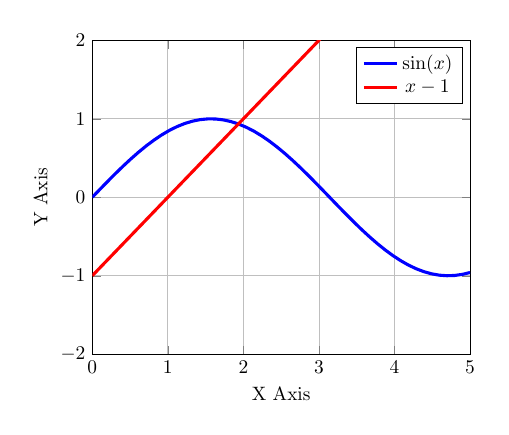
\begin{tikzpicture}[scale=0.7]
			\begin{axis}[
					xmax=5,
					xmin=0,
					ymax=2,
					ymin=-2,
					samples=50,
					grid=major,
					xlabel={X Axis},
					ylabel={Y Axis},
				]
				\addplot[blue, ultra thick,domain=0:5]{sin(deg(x))};
				\addplot[red, ultra thick,domain=0:5]{x-1};
				\legend{$\sin(x)$,$x-1$}
			\end{axis}
		\end{tikzpicture}
		\caption{Plot of the equation $\sin(x)=x-1$}
		\label{sketch:exm-continuous-opposite-signs:2}
	\end{figure}
\end{exm}

\begin{thm}\label{thm-intermediate-value-theorem}
	Let $f:[a,b]\to\mathbb{R}$ be a continuous function, and let $y_0$ be a value
	between $f(a)$ and $f(b)$. Then there exists an $x_0\in(a,b)$ such that
	\footnote{This a generalization of \pref{theorem}{thm-continuous-opposite-signs}}
	$f(x_0)=y_0$. \textit{Remark}: This theorem is also known as the intermediate
	value theorem.
\end{thm}

\begin{proof}
	Of \pref{theorem}{thm-intermediate-value-theorem}.
	\begin{flushleft}
		Assume \gls{wlog} that $f(a)<y_0<f(b)$. Then define $g(x)=f(x)-y_0$. By
		\pref{theorem}{thm-arithmetic-continuous} this function is also continuous on $[a,b]$.
		Therefore,
		\begin{align*}
			 & g(a)=f(a)-y_0<0, \\
			 & g(b)=f(b)-y_0>0
		\end{align*}
	\end{flushleft}
	By \pref{theorem}{thm-continuous-opposite-signs} there exists an $x_0$ such that
	$g(x_0)=0$. Therefore, $f(x_0)=y_0$.
\end{proof}

\begin{thm}\label{thm-weierstrass-theorems}
	Let $f:[a,b]\to\mathbb{R}$ be a continuous function. Weierstrass states the
	following two theorems:
	\begin{enumerate}
		\item The function $f$ is bounded.
		\item The function $f$ assumes a minimum and a maximum.
	\end{enumerate}
\end{thm}

\begin{thm}\label{thm-monotone-closed-interval}
	Let $f:[a,b]\to\mathbb{R}$ be a monotone function. Then, $f$ is continuous
	\textit{iff} the image of $f$ is a closed interval.
\end{thm}

\begin{proof}
	Of theorem (\ref{thm-monotone-closed-interval}).
	\begin{flushleft}
		By \pref{theorem}{thm-weierstrass-theorems}, statement 2, the function $f$
		assumes a minimum $m$ and maximum $M$. The image of $f$ is $[m,M]$ because
		$f$ obtains any value $y_0\in(m,M)$ by \pref{the intermediate value theorem}{thm-intermediate-value-theorem}.
	\end{flushleft}
\end{proof}

\begin{thm}\label{thm-continuous-monotone-invertible}
	If $f$ is continuous and strictly monotone, then $f$ is invertible whose
	inverse function is also continuous and monotone.
\end{thm}


\section{Single Variable Calculus}

TODO: Add descriptions


\subsection{Derivatives}\label{subsec-derivatives}

\begin{definition}\label{def-differentiable}
	We say that a function $f$ is differentiable at $x_0$ if the limit in
	\pref{equation}{eq-differentiable} exists and is finite. The (first) derivative
	of $f$ at $x_0$ is equal to the result of this limit and is denoted by
	\begin{equation}\label{eq-differentiable}
		\lim_{x \to x_0}\frac{f(x)-f(x_0)}{x-x_0} \defines f^\prime(x_0) = \frac{\diff f}{\diff x}(x_0)
	\end{equation}
\end{definition}

\begin{rem}\label{rem-differentiable}
	The limit in \pref{definition}{def-differentiable} is equivalent to
	\begin{equation}\label{eq-differentiable-alt}
		f^\prime(x_0)=\lim_{h \to 0}\frac{f(x_0+h)-f(x_0)}{h}
	\end{equation}
	You can convince yourself that these definitions are equivalent by substituting
	$h\defines x-x_0$.
\end{rem}

\begin{definition}
	If $f$ is differentiable at $x_0$, then
	\begin{equation}
		y = f^\prime(x_0)(x-x_0)+f(x_0)
	\end{equation}
	is called the tangent line of $f$ at $x_0$.
\end{definition}

\begin{exm}\label{exm-derivatives:1}
	Let $f(x)=c$. For any $x_0\in\domain{f}$,
	\begin{align*}
		f^\prime(x_0) & = \lim_{x \to x_0}\frac{c-c}{x-x_0} \\
		              & = 0
	\end{align*}
\end{exm}

\begin{exm}\label{exm-derivatives:2}
	Let $f(x)=x$. For any $x_0\in\domain{f}$,
	\begin{align*}
		f^\prime(x_0) & = \lim_{x \to x_0}\frac{x-x_0}{x-x_0} \\
		              & = 1
	\end{align*}
\end{exm}

\begin{exm}\label{exm-derivatives:3}
	Let $f(x)=x^2$. For any $x_0\in\domain{f}$,
	\begin{align*}
		f^\prime(x_0) & = \lim_{x \to x_0}\frac{x^2-x_0^2}{x-x_0}      \\
		              & = \lim_{x \to x_0}\frac{(x-x_0)(x+x_0)}{x-x_0} \\
		              & = \lim_{x \to x_0} \left(x+x_0\right)          \\
		              & = 2x_0
	\end{align*}
\end{exm}

\begin{exm}\label{exm-derivatives:4}
	Let $f(x)=\sqrt{x}$. For any\footnote{This function in particular is not
		differentiable in the origin} $x_0\in\domain{f}:x_0>0$,
	\begin{align*}
		f^\prime(x_0) & = \lim_{x \to x_0}\frac{\sqrt{x}-\sqrt{x_0}}{x-x_0}                                               \\
		              & = \lim_{x \to x_0}\frac{(\sqrt{x}-\sqrt{x_0})(\sqrt{x}+\sqrt{x_0})}{(x-x_0)(\sqrt{x}+\sqrt{x_0})} \\
		              & = \lim_{x \to x_0}\frac{x-x_0}{(x-x_0)(\sqrt{x}+\sqrt{x_0})}                                      \\
		              & = \lim_{x \to x_0}\frac{1}{\sqrt{x}+\sqrt{x_0}}                                                   \\
		              & = \frac{1}{2\sqrt{x_0}}
	\end{align*}
\end{exm}

\begin{exm}\label{exm-derivatives:5}
	Let $f(x)=\sin(x)$. For any $x_0\in\domain{f}$,
	\begin{align*}
		f^\prime(x_0) & = \lim_{x \to x_0}\frac{\sin(x)-\sin(x_0)}{x-x_0}                                                                                                                                                               \\
		              & = \lim_{x \to x_0}\frac{2\sin\left(\frac{x-x_0}{2}\right)\cos\left(\frac{x+x_0}{2}\right)}{x-x_0}                                                                                                               \\
		              & = \lim_{x \to x_0}\left(\frac{\sin\left(\frac{x-x_0}{2}\right)}{\frac{x-x_0}{2}}\right)\lim_{x \to x_0}\left(\cos\left(\frac{x+x_0}{2}\right)\right) &  & \text{definition (\ref{thm-limit-arithmetic})}        \\
		              & = \cos(x_0)                                                                                                                                          &  & \text{example (\ref{exm-important-sin-over-x-limit})}
	\end{align*}
\end{exm}

\begin{rem}\label{rem-euler-limit}
	We can rewrite theorem (\ref{thm-euler-sequence-monotonicity-increasing}) as
	function, \textit{i.e.}
	\begin{equation}
		\exp(x)\defines\lim_{h \to 0}\left(1+hx\right)^\frac{1}{h}=e
	\end{equation}
\end{rem}

\begin{definition}\label{def-euler-alt}
	An alternative definition of the euler number defines that $e$ is the unique
	positive number for which $f(x_0)=\exp(x_0)$, and
	\begin{align}
		f'(x_0) & = \lim_{h\to0}\frac{f(x_0+h)-f(x_0)}{h}\nonumber                          \\
		        & = \lim_{h\to0}\frac{\exp(x_0+h)-\exp(x_0)}{h}         &  & x_0=0\nonumber \\
		        & = \lim_{h\to0}\frac{\exp(h)-1}{h}\label{eq-euler-alt}                     \\
		        & = 1\nonumber
	\end{align}
\end{definition}

\begin{exm}\label{exm-derivatives:6}
	Let $f(x)=\ln(x)$. For any $x_0\in\domain{f}$,
	\begin{align*}
		f^\prime(x_0) & = \lim_{h \to 0}\frac{\ln(x_0+h)-\ln(x_0)}{h}                                                                                                           \\
		              & = \lim_{h \to 0}\frac{\ln\left(\frac{x+h}{x_0}\right)}{h}                                                                                               \\
		              & = \ln\left(\lim_{h \to 0}\left(\left(1+\frac{h}{x_0}\right)^{\frac{1}{h}}\right)\right) &  & \text{\pref{theorem}{thm-elementary-functions-continuous}} \\
		              & = \ln\left(\exp\left(\frac{1}{x_0}\right)\right)                                        &  & \text{\pref{remark}{rem-euler-limit}}                      \\
		              & = \frac{1}{x_0}
	\end{align*}
\end{exm}

\begin{exm}\label{exm-derivatives:7}
	Let $f(x)=\abs{x}$. For $x=0$ this limit does not exists because
	\begin{align*}
		f^\prime(x_0) & = \lim_{x \to 0}\frac{\abs{x}-\abs{0}}{x-0} \\
		              & = \lim_{x \to 0}\frac{\abs{x}}{x}
	\end{align*}
	but notice that this limit doesn't exists since
	\begin{equation*}
		\lim_{x \to 0^+}\frac{x}{x} = 1 \neq -1 = \lim_{x \to 0^-}\frac{-x}{x}
	\end{equation*}
	wherefore the derivative of the absolute value function \gls{dne} in the origin.
\end{exm}

\begin{rem}
	In \pref{example}{exm-derivatives:6} we saw why functions are not differentiable
	at cusps.
\end{rem}

\begin{thm}\label{thm-differentiability-implies-continuity}
	If the function $f$ is differentiable at $x_0$, then $f$ is continuous at $x_0$.
\end{thm}

\begin{proof}
	Of \pref{theorem}{thm-differentiability-implies-continuity}.
	\begin{flushleft}
		One of the prerequisites of this theorem are that the limit stated in
		\pref{definition}{def-differentiable} exists. Therefore,
		\begin{align*}
			\lim_{x \to x_0}\left(f(x)-f(x_0)\right) & = \underbrace{\lim_{x \to x_0}\left(\frac{f(x)-f(x_0)}{x-x_0}\right)}_{=f^\prime(x_0)}\cdot\underbrace{\lim_{x \to x_0}(x-x_0)}_{=0}                                                     \\
			                                         & =  0                                                                                                                                 &  & \text{\pref{definition}{thm-limit-arithmetic}} \\
		\end{align*}
		But this means $f(x)\tolim{x}{x_0}0$.
		So, by \pref{definition}{def-continuity-at-point-a}, $f$ is continuous at
		the point $x_0$.
	\end{flushleft}
\end{proof}

\begin{rem}\label{rem-continuity-doesnt-imply-differentiability}
	It is very important to point out that the converse of \pref{theorem}{thm-differentiability-implies-continuity}
	is false, \textit{i.e.} continuity does not imply differentiability. See \pref{example}{exm-derivatives:6}
	why this couldn't possibly be true. However, if $f$ is not continuous, then $f$ is not differentiable, either.
\end{rem}

\begin{definition}\label{def-one-sided-derivatives}
	Similar to \pref{definition}{def-differentiable}, we can define one-sided derivatives by
	\begin{equation}\label{eq-right-sided-derivative}
		f_+^\prime(x)=\lim_{x \to x_0^+}\frac{f(x)-f(x_0)}{x-x_0}
	\end{equation}
	\begin{equation}\label{eq-left-sided-derivative}
		f_-^\prime(x)=\lim_{x \to x_0^-}\frac{f(x)-f(x_0)}{x-x_0}
	\end{equation}
	if the limit exists.
\end{definition}

\begin{thm}\label{thm-derivative-arithmetic}
	Let $f$ and $g$ be two differentiable functions, and $c\in\mathbb{R}$. Then
	\begin{enumerate}
		\item $(c\cdot f)^\prime(x_0) = c \cdot f^\prime(x_0)$
		\item $(f \pm g)^\prime(x_0) = f^\prime(x_0) \pm g^\prime(x_0)$
		\item $(f \cdot g)^\prime(x_0) = f^\prime(x_0) \cdot g(x_0) + g^\prime(x_0) \cdot f(x_0)$
		\item $\left(\tfrac{f}{g}\right)^\prime(x_0) = \tfrac{f^\prime(x_0)\cdot g(x_0) - g^\prime(x_0) \cdot f(x_0)}{g^2(x_0)}$ if $g(x_0)\neq0$
	\end{enumerate}
\end{thm}

\begin{proof}
	Of \pref{theorem}{thm-derivative-arithmetic}.
	\begin{flushleft}
		\textbf{Product Rule}:
		\begin{align*}
			(f \cdot g)^\prime(x_0) & = \lim_{h \to 0}\frac{f(x_0+h) g(x_0+h)-f(x_0) g(x_0)}{h}                                                           \\
			                        & = \lim_{h \to 0}\left(\frac{1}{h}\big( f(x_0+h) g(x_0+h) - f(x_0)(x_0+h) +f(x_0)(x_0+h) - f(x_0) g(x_0)\big)\right) \\
			                        & = \lim_{h \to 0}\left(g(x_0+h)\frac{f(x_0+h)-f(x_0)}{h}+f(x_0)\frac{g(x_0+h)-g(x_0)}{h}\right)                      \\
			                        & = g(x_0) \cdot f^\prime(x_0) + f(x_0) \cdot g^\prime(x_0)
		\end{align*}
		Notice that in the last step we used the fact that by \pref{theorem}{thm-differentiability-implies-continuity},
		$g$ is continuous which is an important detail required in this proof that explains why
		$g(x_0+h)\tolim{h}{0}g(x_0)$.
	\end{flushleft}
\end{proof}

\begin{thm}\label{thm-chain-rule}
	If $f$ is differentiable at $x_0$ and $g$ is differentiable at $f(x_a)$, then
	\begin{equation}\label{eq-chain-rule}
		(g \circ f)^\prime(x_0) = \underbrace{g^\prime(f(x_0))}_{\text{outer derivative}} \cdot \underbrace{f^\prime(x_0)}_{\text{inner derivative}}
	\end{equation}
	This is called the chain rule.
\end{thm}

\begin{thm}\label{thm-derivative-of-inverse-function}
	Let $y=f(x)$ be invertible, continuous at a neighborhood of $x_0$, and differentiable
	at $x_0$. Also assume that $f^\prime(x_0)\neq0$. Then $x=f^{-1}(y)$ is differentiable
	at $y_0=f(x_0)$, and
	\begin{equation}\label{eq-derivative-of-inverse-function}
		\left(f^{-1}\right)^\prime(y_0)=\frac{1}{f^\prime(x_0)}
	\end{equation}
\end{thm}

\begin{exm}\label{exm-derivative-of-inverse-function:1}
	We know that for all $x>0$, $(\ln(x))^\prime=\tfrac{1}{x}$. The inverse function
	of $y=\ln(x)$ is $x=e^y$. Hence, by \pref{theorem}{thm-derivative-of-inverse-function}
	we can write
	\begin{equation*}
		(e^y)^\prime = \frac{1}{\ln(x)^\prime} = \frac{1}{x^{-1}} = e^y
	\end{equation*}
	where we used the result obtained from \pref{example}{exm-derivatives:5}.
\end{exm}

\begin{exm}\label{exm-derivative-of-inverse-function:2}
	Let $f(x)=\sin(x)=y$ and $f^{-1}(x)=\arcsin(y)$. Hence, by
	\pref{theorem}{thm-derivative-of-inverse-function} we can write
	\begin{align*}
		(\arcsin(y))^\prime & = \frac{1}{\sin(x)^\prime}     \\
		                    & = \frac{1}{\cos(x)}            \\
		                    & = \frac{1}{\sqrt{1-\sin^2(x)}} \\
		                    & = \frac{1}{\sqrt{1-y^2}}
	\end{align*}
\end{exm}

\begin{exm}\label{exm-derivative-of-inverse-function:3}
	Let $f(x)=\tan(x)=y$ and $f^{-1}(x)=\arctan(y)$. Hence, by
	\pref{theorem}{thm-derivative-of-inverse-function} we can write TODO
\end{exm}

\begin{rem}\label{rem-first-derivative-polynomial}
	Let $f(x)=x^\alpha$ with $\alpha\in\mathbb{R}$ and $x>0$. Define
	$g(x)\defines \ln(f(x))$. By using the chain rule we get that
	\begin{equation}\label{eq-first-derivative-polynomial:1}
		g^\prime(x) = \frac{1}{f(x)} \cdot f^\prime(x)
	\end{equation}
	On the other hand,
	\begin{equation}\label{eq-first-derivative-polynomial:2}
		g(x) = \ln(x^\alpha) = \alpha\ln(x) \implies g^\prime(x) = \frac{\alpha}{x}
	\end{equation}
	So by \pref{equation}{eq-first-derivative-polynomial:1} and \pref{equation}{eq-first-derivative-polynomial:2},
	\begin{align*}
		\frac{1}{f(x)} \cdot f^\prime(x) = \frac{\alpha}{x} \implies f^\prime(x) = \alpha \cdot x^{\alpha-1}
	\end{align*}
\end{rem}


\subsection{Higher Order Derivatives}\label{subsec-higher-order-derivatives}

\begin{definition}\label{def-higher-order-derivatives}
	We define the $n$-th derivative by recursion as the $(n-1)$-th derivative of
	the function $f$ and denote it in Leibniz notation by
	\begin{equation}
		f^{(n)}(x) = \frac{\diff^n f}{\diff x^n}
	\end{equation}
	if $f$ is $n$-times differentiable.
\end{definition}

\begin{rem}
	The zeroth derivative of a function is just the original function.
\end{rem}

\begin{thm}\label{thm-higher-order-derivative-arithmetic}
	Let $f$ and $g$ be two differentiable functions, and $c\in\mathbb{R}$. Then
	\footnote{Recall that $\binom{n}{k}=\tfrac{n!}{k!(n-k)!}$}
	\begin{enumerate}
		\item $(c\cdot f)^{(n)}(x_0) = c \cdot f^{(n)}(x_0)$
		\item $(f \pm g)^{(n)}(x_0) = f^{(n)}(x_0) \pm g^{(n)}(x_0)$
		\item $(f \cdot g)^{(n)}(x_0) = \sum_{k=0}^n \binom{n}{k}f^{(k)}(x_0) \cdot g^{(k-1)}(x_0)$
	\end{enumerate}
	The third item in this list is also called Leibniz' formula.
\end{thm}

\begin{exm}
	Let $f(x)=x^2e^x$. Find the $9$-th derivative of this function.
	\begin{flushleft}
		\textbf{Answer}: By \pref{theorem}{thm-higher-order-derivative-arithmetic},
		we have that
		\begin{align*}
			(x^2e^x)^{(9)} & = \sum_{k=0}^9\binom{9}{k}(x^2)^{(k)}(e^x)^{(k)}                                                                                \\
			               & = \left(\binom{9}{0}x^2+\binom{9}{1}2x+\binom{9}{2}2\right)e^x &  & \text{\pref{example}{exm-derivative-of-inverse-function:1}} \\
			               & = \left(x^2+18x+72\right)e^x
		\end{align*}
	\end{flushleft}
\end{exm}

\subsubsection{Fermats Theorem for Extrema}\label{subsubsec-fermtas-theorem-extrema}

\begin{thm}\label{thm-fermats-theorem-extrema}
	Let $f(x)$ be a function defined on $(a,b)$ and let this function take on
	a maximum (or minimum) value at some point $c\in(a,b)$. Fermat's theorem for
	extrema states that if $f$ is differentiable, then
	\begin{equation}
		f^\prime(c)=0
	\end{equation}
\end{thm}

\begin{proof}
	Of \pref{theorem}{thm-fermats-theorem-extrema}.
	\begin{flushleft}
		\gls{wlog} assume that $x_0$ is a maximum. Since $f$ is differentiable
		we can write
		\begin{align*}
			f^\prime(x_0) & = \lim_{x \to x_0}\frac{f(x)-f(x_0)}{x-x_0}   \\
			              & = \lim_{x \to x_0^+}\frac{f(x)-f(x_0)}{x-x_0} \\
			              & = \lim_{x \to x_0^-}\frac{f(x)-f(x_0)}{x-x_0}
		\end{align*}
		Now consider all $x>x_0$; it follows that
		\begin{align}
			 & x-x_0>0\nonumber                                                                     \\
			\implies
			 & f(x)-f(x_0)\leq0\nonumber                                                            \\
			\implies
			 & \frac{f(x)-f(x_0)}{x-x_0}\leq0\nonumber                                              \\
			\implies
			 & \lim_{x \to x_0^+}\frac{f(x)-f(x_0)}{x-x_0}\leq0\label{eq-fermats-theorem-extrema:1}
		\end{align}
		Next consider where $x<x_0$; then
		\begin{align}
			 & x-x_0<0\nonumber                                                                     \\
			\implies
			 & f(x)-f(x_0)\leq0\nonumber                                                            \\
			\implies
			 & \frac{f(x)-f(x_0)}{x-x_0}\geq0\nonumber                                              \\
			\implies
			 & \lim_{x \to x_0^-}\frac{f(x)-f(x_0)}{x-x_0}\geq0\label{eq-fermats-theorem-extrema:2}
		\end{align}
		In summary, \pref{equation}{eq-fermats-theorem-extrema:1} and \pref{equation}{eq-fermats-theorem-extrema:2}
		imply that
		\begin{equation*}
			f^\prime(x_0)=0
		\end{equation*}
	\end{flushleft}
\end{proof}

\begin{rem}
	In high school we often used implicitly \pref{theorem}{thm-fermats-theorem-extrema}
	to find candidates for maxima and minima values. But this theorem doesn't find
	\textit{all} possible candidates. Take for instance the absolute value function.
	It obviously has a minimum in the origin, but Fermat's theorem for extrema is not
	going to pick up this candidate since $f(x)=\abs{x}$ is not differentiable at $x=0$.
	On the other side, this theorem may even yield candidates that neither maxima nor
	minima (take for instance $f(x)=x^3$ at $x=0$) so you have to use this theorem with
	caution. It is not by accident that these values are referred to as \enquote{candidates}.
	They may or may not promote to extrema depending on the actual function.
\end{rem}

\subsubsection{Rolle's Theorem}\label{subsubsec-rolles-theorem}

\begin{thm}\label{thm-rolles-theorem}
	Let $a,b\in\mathbb{R}$ where $a<b$. Let $f$ be a continuous in $[a,b]$ and
	differentiable in $(a,b)$ subject to the condition \cite[p.169]{wuest2009} that
	\begin{equation*}
		f(a)=f(b)
	\end{equation*}
	Then there exists a $c\in(a,b)$ such that
	\begin{equation}
		f^\prime(c)=0
	\end{equation}
\end{thm}

\begin{proof}
	Of theorem (\ref{thm-rolles-theorem}).
	\begin{flushleft}
		Since $f$ is continuous on $[a,b]$, by \pref{theorem}{thm-weierstrass-theorems}
		it has a minimum $m$ and a maximum $M$. If $m=M$, then $f$ must be a constant
		function in which case we are done (\textit{cf.} \pref{example}{exm-derivatives:1}).
		But if we rule out this possibility, then $m<M$ implies that at least one
		the these extrema is not obtained at the endpoints of this interval since the
		theorem assumes that $f(a)=f(b)$ but $f(m)\neq f(M)$. Denote the extrema
		that is not an endpoint by $c\in(a,b)$. Because the function is differentiable
		in $(a,b)$, by \pref{theorem}{thm-fermats-theorem-extrema} we know that $f^\prime(c)=0$.
	\end{flushleft}
\end{proof}

\subsubsection{Mean Value Theorem}\label{subsubsec-mean-value-theorem}

\begin{thm}\label{thm-mean-value-theorem}
	Let $a,b\in\mathbb{R}$ where $a<b$. Let $f$ be continuous in $[a,b]$ and
	differentiable in $(a,b)$. Then there exists a $c\in(a,b)$ such that
	\footnote{This is also known as Lagrange's theorem}
	\begin{equation}
		f^\prime(c)=\frac{f(b)-f(a)}{b-a}
	\end{equation}
\end{thm}

\begin{proof}
	Of \pref{theorem}{thm-mean-value-theorem}.
	\begin{flushleft}
		We define a new function $F$ such that
		\begin{equation*}
			F(x)=f(x)-\underbrace{\left(f(a)+\frac{f(b)-f(a)}{b-a}(x-a)\right)}_{\text{secant line}}
		\end{equation*}
		Then \pref{theorem}{thm-arithmetic-continuous}, $F$ is continuous on $[a,b]$
		because $f$ was also continuous. It's also differentiable on $(a,b)$ for
		precisely the same reason, \textit{cf.} \pref{theorem}{thm-derivative-arithmetic}.
		Notice also that $F(a)=F(b)=0$. So, by \pref{theorem}{thm-rolles-theorem} there
		exists a $c\in(a,b)$ such that $F^\prime(c)=0$. Then
		\begin{align*}
			F^\prime(c) & = f^\prime(c) - \frac{f(b)-f(a)}{b-a} \\
			            & = 0
		\end{align*}
		Hence,
		\begin{equation*}
			f^\prime(c)=\frac{f(b)-f(a)}{b-a}
		\end{equation*}
	\end{flushleft}
\end{proof}

\subsubsection{Cauchy's Theorem}\label{subsubsec-cauchys-theorem}

\begin{thm}\label{thm-cauchys-theorem}
	Let $f(x)$ and $g(x)$ be continuous in $[a,b]$ and differentiable in $(a,b)$.
	Assume that $\forall x\in(a,b)$, $g^\prime(x)=0$. Then Cauchy's theorem states
	that
	\begin{enumerate}
		\item $g(a)\neq g(b)$
		\item $\exists c\in(a,b)$ s.t.
		      \begin{equation}
			      \frac{f^\prime(x)}{g^\prime(x)}=\frac{f(b)-f(a)}{g(b)-g(a)}
		      \end{equation}
	\end{enumerate}
\end{thm}

\begin{thm}\label{thm-differentiable-constant-zero}
	Let $f$ be a differentiable function defined on $(a,b)$. The function is constant
	\textit{iff} for any $x\in(a,b)$, $f^\prime(x)=0$.
\end{thm}

\begin{proof}
	Of \pref{theorem}{thm-differentiable-constant-zero}.
	\begin{flushleft}
		\proofright: We already proved this direction in \pref{example}{exm-derivatives:1}.
	\end{flushleft}
	\begin{flushleft}
		\proofleft: \gls{wlog} take any two points $x,y\in(a,b)$ such that $a<x<y<b$.
		By \pref{theorem}{thm-mean-value-theorem} on $[x,y]$, there exists a point
		$c\in(x,y)$ such that
		\begin{equation*}
			f^\prime(c) = \frac{f(y)-f(x)}{y-x} = 0
		\end{equation*}
		Hence, $f(y)=f(x)$. Therefore, $f$ is a constant function.
	\end{flushleft}
\end{proof}

\begin{thm}\label{thm-differentiable-strictly-monotone}
	Let $f$ be a differentiable function on $(a,b)$. If $f^\prime(x)>0$ for any
	$x\in\domain{f}$, then $f$ is strictly monotonically increasing. Conversely,
	if $f^\prime(x)<0$, then $f$ is strictly monotonically decreasing.
\end{thm}

\begin{proof}
	Of \pref{theorem}{thm-differentiable-strictly-monotone}.
	\begin{flushleft}
		\gls{wlog}, take any $a<x<y<b$. By \pref{theorem}{thm-mean-value-theorem},
		there is a point $c\in[x,y]$ such that
		\begin{equation}
			\frac{f^\prime(x)}{g^\prime(x)}=\frac{f(b)-f(a)}{g(b)-g(a)}
		\end{equation}
		Since $f^\prime(c)>0$ it follows that $f(y)>f(x)$. Hence, by
		\pref{definition}{def-monotonicity}, $f$ is strictly monotonically increasing.
	\end{flushleft}
\end{proof}

\begin{rem}\label{rem-differentiable-strictly-monotone}
	The converse of \pref{theorem}{thm-differentiable-strictly-monotone} is false,
	\textit{i.e.} if $f$ is strictly monotonically increasing or decreasing, then its
	first derivative is either strictly positive or negative, respectively. Take for
	instance $f(x)=x^3$. This function is strictly increasing on the entire real line,
	but its derivative at $x=0$ is zero. But what we can say is that
	\begin{equation}\label{eq-differentiable-strictly-monotone}
		\left(f\text{ is differentiable } \implies f^\prime\geq0\right)
		\iff f\text{ is monotonically increasing}
	\end{equation}
\end{rem}

\begin{exm}\label{exm-differentiable-strictly-monotone}
	Let $f(x)=\arctan(x)$. This function is strictly increasing on $\mathbb{R}$,
	since $f^\prime(x)=\tfrac{1}{1+x^2}>0$ for all $x\in\mathbb{R}$. Next consider
	the function $g(x)=\tfrac{1}{x}$. Then $g^\prime(x)=-\tfrac{1}{x^2}<0$ for any
	$x\neq0$, so this function is strictly monotonically decreasing.
\end{exm}


\subsection{Curve Sketching}\label{subsec-curve-sketching}

\begin{definition}\label{def-local-minimum-maximum}
	A point $x_0$ is called a local minimum if $f(x) \geq f(x_0)$ for all $x$ in
	a neighborhood of $x_0$. Likewise, it is called a local maximum if $f(x) \geq f(x_0)$
	for all $x$ in a neighborhood of $x_0$.
\end{definition}

\begin{definition}\label{def-extrema}
	We will call $x_0$ a local extrema if $x_0$ is a local minimum or maximum.
\end{definition}

\begin{definition}\label{def-critical-point}
	We will call $x_0$ a critical point if $f^\prime(x_0)=0$ or $f$ is not differentiable
	at $x_0$.
\end{definition}

\begin{thm}\label{thm-first-derivative-test}
	Let $x_0$ be a critical point of $f$, and assume that $f$ is continuous at $x_0$
	and differentiable in a neighborhood of $x_0$, although possibly not differentiable
	at $x_0$ itself. Then the first derivative test states that
	\begin{enumerate}
		\item if $f^\prime(x_0)$ changes signs from minus to plus, then
		      $x_0$ is local minimum.
		\item if $f^\prime(x_0)$ changes signs from plus to minus, then
		      $x_0$ is local maximum.
		\item if $f^\prime(x_0)$ does not change signs, then $x_0$ is not an
		      extremum.
	\end{enumerate}
\end{thm}

\begin{thm}\label{thm-second-derivative-test}
	Let $x_0$ be a critical point of $f$, and assume that $f$ is differentiable twice
	at $x_0$. Then the second derivative test states that
	\begin{enumerate}
		\item if $f''(x_0)>0$, then $x_0$ is local minimum.
		\item if $f''(x_0)<0$, then $x_0$ is local maximum.
		\item if $f''(x_0)=0$, then this theorem doesn't reveal any additional
		      information about $x_0$
	\end{enumerate}
\end{thm}

\begin{thm}\label{thm-darboux-theorem}
	Let $f$ be a differentiable function on $[a,b]$ (with one-sided derivatives
	at the points of this interval, \textit{i.e.} $f_+^\prime(a)$ and $f_-^\prime(b)$
	exists) and let $c$ be value between $f_+^\prime(a)$ and $f_-^\prime(b)$.
	Then Darboux theorem\footnote{This is sort of an
		\hyperref[thm-intermediate-value-theorem]{intermediate value theorem}
		for derivatives.} states that there exists an $x_0$ such that $f'(x_0)=c$.
\end{thm}

\begin{crl}\label{crl-darboux-theorem}
	If $f$ is differentiable on $[a,b]$, then $f'$ may have points of infinite
	discontinuities (as they were defined in definition (\ref{def-infinite-discontinuity})).
\end{crl}

\begin{rem}\label{rem-darboux-theorem}
	The derivative of $f$ never can have removable or jump discontinuities without
	violating \hyperref[thm-darboux-theorem]{Darboux theorem}.
\end{rem}

\begin{exm}
	Consider the function
	\begin{equation*}
		f(x)=\begin{cases}
			\abs{x}^\frac{3}{2}\sin\left(\frac{1}{x}\right)\text{ if }x\neq0 \\
			0\text{ else }
		\end{cases}
	\end{equation*}
	Show that $f'$ is not continuous at $x=0$.
	\begin{flushleft}
		\textbf{Answer}: TODO
	\end{flushleft}
\end{exm}

\begin{thm}\label{thm-lhopitals-rule}
	Let $f$ and $g$ be two differentiable functions in a neighborhood of $x=a$,
	although possibly not in the neighborhood of $x$ itself. Assume that
	\begin{equation*}
		\lim_{x \to a}f(x)=\lim_{x \to a}g(x)=0
	\end{equation*}
	and that $g'(x)\neq0$ for all $x \neq a$ near $a$. Assume further that the limit
	\begin{equation*}
		\lim_{x \to a}\frac{f'(x)}{g'(x)}
	\end{equation*}
	exists. If all these conditions are met, then L'H{\^o}pital's rule says that
	\begin{equation}
		\lim_{x \to a}\frac{f(x)}{g(x)}=\lim_{x \to a}\frac{f'(x)}{g'(x)}
	\end{equation}
\end{thm}

\begin{rem}\label{rem-lhopitals-rule}
	In L'H{\^o}pital's rule we find many theorems bundled together that allow us
	under certain conditions to calculate limits of the form \enquote{$\tfrac{\infty}{\infty}$}
	or \enquote{$\tfrac{0}{0}$}.
\end{rem}

\begin{exm}\label{exm-lhopitals-rule:1}
	Consider the function $f(x)=\tfrac{\sin(x)}{x}$. Find the limit of $f$ as $x\to0$.
	\begin{flushleft}
		\textbf{Answer}: By \pref{theorem}{thm-lhopitals-rule} we get that
		\begin{align*}
			\lim_{x\to0}\frac{\sin(x)}{x} & = \lim_{x\to0}\frac{\cos(x)}{1} \\
			                              & = 1
		\end{align*}
	\end{flushleft}
	Note that this was much easier to find than in \pref{example}{exm-important-sin-over-x-limit}.
\end{exm}

\begin{exm}\label{exm-lhopitals-rule:2}
	Consider the function $f(x)=\tfrac{\ln(x)}{x-1}$. Find the limit of $f$ as $x\to1$.
	\begin{flushleft}
		\textbf{Answer}: By \pref{theorem}{thm-lhopitals-rule} we get that
		\begin{align*}
			\lim_{x\to1}\frac{\ln(x)}{x-1} & = \lim_{x\to1}\frac{\frac{1}{x}}{1} \\
			                               & = 1
		\end{align*}
	\end{flushleft}
\end{exm}

\begin{exm}\label{exm-lhopitals-rule:3}
	Consider the function $f(x)=\tfrac{\sin(x)-x}{\tan(x)-x}$. Find the limit of $f$ as $x\to0$.
	\begin{flushleft}
		\textbf{Answer}: By \pref{theorem}{thm-lhopitals-rule} we get that
		\begin{align*}
			\lim_{x\to0}\frac{\sin(x)-x}{\tan(x)-x} & = \lim_{x\to0}\frac{\cos(x)-1}{\frac{1}{\cos^2(x)}}                      \\
			                                        & = \lim_{x\to0}\frac{-\sin(x)}{-2\cdot\frac{1}{\cos^3(x)}\cdot(-\sin(x))} \\
			                                        & = -\frac{1}{2}
		\end{align*}
	\end{flushleft}
\end{exm}

\begin{exm}\label{exm-lhopitals-rule:4}
	Consider the function $f(x)=x\ln(x)$. Find the limit of $f$ as $x\to0^+$.
	\begin{flushleft}
		\textbf{Answer}: By \pref{theorem}{thm-lhopitals-rule} we get that
		\begin{align*}
			\lim_{x\to0^+}x^x & = \lim_{x\to0^+}\frac{\ln(x)}{\frac{1}{x}}         \\
			                  & = \lim_{x\to0^+}\frac{\frac{1}{x}}{-\frac{1}{x^2}} \\
			                  & = \lim_{x\to0^+}\left(-x\right)                    \\
			                  & = 0
		\end{align*}
	\end{flushleft}
\end{exm}

\begin{exm}\label{exm-lhopitals-rule:5}
	Consider the function $f(x)=x^x$. Find the limit of $f$ as $x\to0^+$.
	\begin{flushleft}
		\textbf{Answer}: By \pref{theorem}{thm-lhopitals-rule} we get that
		\begin{align*}
			\lim_{x\to0^+}x^x & = \lim_{x\to0^+}e^{\ln\left(x^x\right)}                                                  \\
			                  & = \lim_{x\to0^+}e^{x\ln(x)}             &  & \text{example (\ref{exm-lhopitals-rule:4})} \\
			                  & = 1
		\end{align*}
	\end{flushleft}
\end{exm}

\begin{definition}\label{def-convex-concave-functions}
	A function is called convex on $I$ if for all $x,y\in I$ the secant connecting
	the point $(x,f(x))$ to the point $(y,f(y))$ is above the graph. Conversely,
	a function is called concave if for all $x,y\in I$ the secant connecting
	the point $(x,f(x))$ to the point $(y,f(y))$ is below the graph.
\end{definition}

\begin{thm}\label{thm-convex-concave-first-derivative}
	Let $f$ be a differentiable function on $(a,b)$. Then
	\begin{enumerate}
		\item $f$ is convex \textit{iff} the graph is above the tangent line at any $x_0\in(a,b)$.
		\item $f$ is convex \textit{iff} $f'$ is increasing
		\item $f$ is concave \textit{iff} the graph is below the tangent line at any $x_0\in(a,b)$.
		\item $f$ is concave \textit{iff} $f'$ is decreasing
	\end{enumerate}
\end{thm}

\begin{thm}\label{thm-convex-concave-second-derivative}
	Let $f$ be a twice differentiable function on $(a,b)$. Then
	\begin{enumerate}
		\item $f$ is convex \textit{iff} $f''\geq0$
		\item $f$ is concave \textit{iff} $f''<0$
	\end{enumerate}
\end{thm}

\begin{thm}\label{thm-convex-minimum}
	Let $f$ be a convex differentiable function on $(a,b)$, and let $x_0$ be a
	critical point of $f$. Then $x_0$ is a minimum.
\end{thm}

\begin{thm}\label{thm-concave-maximum}
	Let $f$ be a concave differentiable function on $(a,b)$, and let $x_0$ be a
	critical point of $f$. Then $x_0$ is a maximum.
\end{thm}

\begin{definition}\label{def-point-of-inflection}
	We call $x_0$ a point of inflection of $f$ if $f$ is continuous at $x_0$,
	convex on one side of $x_0$ and concave on the other side of $x_0$.
\end{definition}

\begin{rem}\label{rem-point-of-inflection}
	Definition (\ref{def-point-of-inflection}) makes no claim with respect to
	$f''(x_0)=0$ being a satisfactory condition for points of inflection.
\end{rem}

\begin{definition}\label{def-vertical-asymptotes}
	We call $x=x_0$ a vertical asymptote if\footnote{It suffices to require only
		one one-sided limit to diverge to towards either minus or plus infinity}
	\begin{equation}\label{eq-vertical-asymptotes:1}
		\lim_{x \to x_0^+}f(x)= \pm\infty
	\end{equation}
\end{definition}

\begin{definition}\label{def-asymptotes}
	We call $y=ax+b$ an asymptote if
	\begin{equation}\label{eq-asymptotes}
		\lim_{x \to \pm\infty}\left(f(x)-(ax+b)\right)=0
	\end{equation}
\end{definition}

\begin{rem}\label{rem-asymptotes}
	Note that
	\begin{align*}
		f(x)-ax-b                                                                                              & \tolim{x}{\infty}0 \\
		\iff
		\underbrace{\frac{f(x)}{x}}_{\to a}-\underbrace{\frac{ax}{x}}_{\to a}-\underbrace{\frac{b}{x}}_{\to 0} & \tolim{x}{\infty}0
	\end{align*}
	So to find linear asymptotes we can use the following limits:
	\begin{equation}\label{rem-asymptotes:a}
		a = \lim_{x \to \pm\infty}\frac{f(x)}{x}
	\end{equation}
	\begin{equation}\label{rem-asymptotes:b}
		b = \lim_{x \to \pm\infty}\left(f(x)-ax\right)
	\end{equation}
\end{rem}

\begin{exm}\label{exm-curve-sketching}
	Consider the function
	\begin{equation}\label{eq-curve-sketching}
		f(x)=\sqrt[3]{x^2(3-x)}
	\end{equation}
	\begin{flushleft}
		\textbf{Curve Sketching}:
		\begin{enumerate}
			\item The first thing we want to do is to find the domain of the
			      function $f$, which in this case is rather easy: $\domain{f}=\left\{x\in\mathbb{R}\setbuild x\leq3\right\}$.
			\item After that we are interested in the continuity of $f$; since compositions of
			      elementary function are continuous on their entire domain, there is no issue here.
			\item Next we look for points of intersection with the $x$-axis:
			      \begin{align*}
				      f(x) = 0   & = \sqrt[3]{x^2(3-x)} \\
				      \implies x & = 0                  \\
				      \implies x & = 3
			      \end{align*}
			      So the points of intersections are $(0,0)$ and $(3,0)$.
			\item Now we look for the first derivative of $f$. It's easier to find
			      if we rewrite \pref{equation}{eq-curve-sketching} to
			      \begin{equation}\label{eq-curve-sketching:2}
				      f'(x)=x^{\frac{2}{3}}(3-x)^{\frac{1}{3}}
			      \end{equation}
			      Therefore,
			      \begin{equation}\label{eq-curve-sketching:3}
				      f'(x) = \frac{2}{3}x^{-\frac{1}{3}}(3-x)^{\frac{1}{3}} - x^{\frac{2}{3}}\cdot\frac{1}{3}(3-x)^{-\frac{2}{3}}
			      \end{equation}
			      Note that \pref{equation}{eq-curve-sketching:3} is neither defined at
			      $x=0$ nor at $x=3$.
			\item This time we use \pref{theorem}{thm-convex-concave-first-derivative}
			      to find candidates for convex and concave points, \textit{i.e.} if $f' \geq 0$, then
			      \begin{align*}
				      \frac{2}{3}x^{-\frac{1}{3}}(3-x)^{\frac{1}{3}}      & \geq x^{\frac{2}{3}}\cdot\frac{1}{3}(3-x)^{-\frac{2}{3}}                    \\
				      \iff
				      \frac{2}{3}\left(\frac{3-x}{x}\right)^{\frac{1}{3}} & \geq \frac{1}{3}\left(\frac{x}{3-x}\right)^{\frac{2}{3}} &  & \text{if }x>0 \\
				      \iff
				      2(3-x)                                              & \geq x                                                                      \\
				      \iff
				      6-2x                                                & \geq 3x                                                                     \\
				      \iff
				      2                                                   & \geq x
			      \end{align*}
			      So, in the domain $0<x<2$, $f'$ is non-negative. On the other side,
			      if $x<0$ we get that
			      \begin{align*}
				      2(3-x) & \leq x \\
				      \iff
				      2      & \leq x
			      \end{align*}
			      In this case this case we reach a contradictory statement, so no new
			      information was obtained at this step of the calculation. Finally, if
			      $f' \leq 0$ and $x < 0$, then $2 \leq x \neq 3$. In particular, $f'(x=2)=0$.
			\item This step is dedicated to finding the extrema (minimum and maximum)
			      of this function. We can use the results from step (3) to calculate
			      \begin{align*}
				       & x=0 \implies (0,0) \text{ is a local minimum}          &  & \text{\pref{theorem}{thm-convex-minimum}}  \\
				       & x=2 \implies (2,\sqrt[3]{4})\text{ is a local maximum} &  & \text{\pref{theorem}{thm-concave-maximum}}
			      \end{align*}
			\item Now we use \pref{theorem}{thm-second-derivative-test}, the second derivative test:
			      \begin{equation}\label{eq-curve-sketching:4}
				      f''(x) = -2x^{-\frac{4}{3}}(3-x)^{-\frac{5}{3}}
			      \end{equation}
			      Notice that \pref{equation}{eq-curve-sketching:4} is not defined on $x = 0$
			      and $x = 3$. Furthermore, observe that $f'' > 0$ for $x > 3$ and $f'' < 0$ for
			      $0 \neq x < 3$.
			\item Finally it's time to look for points of inflection; we can see
			      from the previous results that there exists only one point of inflection
			      at $x=3$. And because this function is continuous, there exists no vertical
			      asymptote (\textit{cf.} \pref{definition}{def-vertical-asymptotes}) in the
			      domain of $f$. Using \pref{remark}{rem-asymptotes} the linear asymptote ends up being
			      \begin{equation*}
				      y = -x + 1
			      \end{equation*}
			      Last but not least we summarize the information we gathered so
			      far to sketch the curve, see also \pref{figure}{sketch:exm-curve-sketching:1}
			      for the final result.
		\end{enumerate}
	\end{flushleft}
	\begin{figure}[ht!]
		\centering
		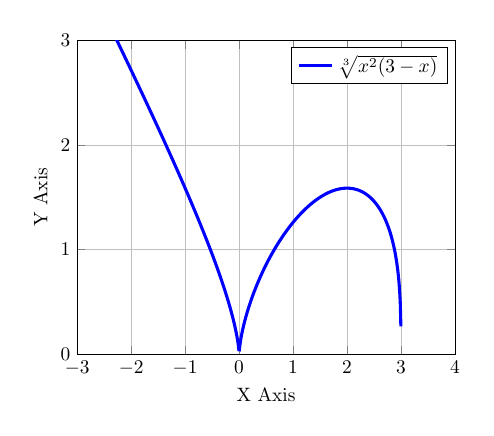
\begin{tikzpicture}[scale=0.7]
			\begin{axis}[
					xmax=4,
					xmin=-3,
					ymax=3,
					ymin=0,
					samples=1000,
					grid=major,
					xlabel={X Axis},
					ylabel={Y Axis},
				]
				\addplot[blue, ultra thick,domain=-5:5]{(x^2*(3-x))^(1/3)};
				\legend{$\sqrt[3]{x^2(3-x)}$}
			\end{axis}
		\end{tikzpicture}
		\caption{Final plot of curve from \pref{example}{exm-curve-sketching}}
		\label{sketch:exm-curve-sketching:1}
	\end{figure}
\end{exm}


\subsection{Taylor Polynomial}\label{subsec-taylor-polynomial}

Under certain conditions on $f$ near $x_0$ we will be able to find for any $\varepsilon>0$
a polynomial $p$ such that $f(x_0)=p(x_0)+R(x_0)$ where $R$ denotes the remainder ($\abs{R(x_0)}<\varepsilon$),
accounting for the inaccuracy of the approximation near $x_0$.

\begin{lemma}\label{lemma-polynomial-derivatives}
	Let $p_n(x)$ be a polynomial of degree $n$ of the function $f$ at the point $x$,
	such that
	\begin{equation}\label{eq-polynomial-derivatives:1}
		p_n(x) = \sum_{k=0}^n \beta_k x^k
	\end{equation}
	Then for any $k\in[0,n]$,
	\begin{equation}\label{eq-polynomial-derivatives:2}
		p_n^{(k)}(x) = \beta_k k!
	\end{equation}
\end{lemma}

\begin{proof}
	Of \pref{lemma}{lemma-polynomial-derivatives}.
	\begin{flushleft}
		If we differentiate the polynomial $p_n(x)$ $k$-times, then
		\begin{itemize}
			\item all terms of degree less than $k$ are zero
			\item for the $k$'th term ($\beta_k x^k$) we get $\beta_k k!$
			\item all terms of degree higher than $k$ disappear at $x=0$
		\end{itemize}
	\end{flushleft}
\end{proof}

\begin{rem}
	By the previous \pref{lemma}{lemma-polynomial-derivatives}, define the coefficients as
	\begin{equation*}
		\beta_k = \frac{p_n^{(k)}(x)}{k!}
	\end{equation*}
\end{rem}

\begin{definition}\label{def-taylor-polynomial}
	Let $n\in\mathbb{N}$ and $f$ be a $n$-times differentiable function at the point
	$x_0\in\domain{f}$. We call \cite[p.214]{wuest2009}
	\begin{equation}\label{eq-taylor-polynomial}
		p_n(f,x_0)(x) \defines \sum_{k=0}^n \frac{f^{(k)}(x_0)}{k!}(x-x_0)^k \qquad(x\in\mathbb{R})
	\end{equation}
	the Taylor polynomial of degree $n$ of the function $f$ at the point $x_0$.
\end{definition}

\begin{definition}\label{def-maclaurin-polynomial}
	The Taylor polynomial introduced in \pref{definition}{def-taylor-polynomial}
	is called Maclaurin polynomial, if $x_0=0$. So,
	\begin{equation}\label{eq-maclaurin-polynomial}
		p_n(f,0)(x) \defines \sum_{k=0}^n \frac{f^{(k)}(0)}{k!}x^k
	\end{equation}
\end{definition}

\begin{exm}\label{exm-sin-taylor-series}
	Find the Maclaurin polynomial for the function $f(x)=\sin(x)$ of degree $3$.
	\begin{flushleft}
		\textbf{Answer}: Since the Maclaurin polynomial evaluates at $x_0=0$,
		we find that
		\begin{align*}
			 & f(x)=\sin(x) \implies f(0)=0         \\
			 & f'(x)=\cos(x) \implies f'(0)=1       \\
			 & f''(x)=-\sin(x) \implies f''(0)=0    \\
			 & f'''(x)=-\cos(x) \implies f'''(0)=-1 \\
		\end{align*}
		So the polynomial is
		\begin{align*}
			p_3(\sin,0) & = f(0) + f'(0)x + \frac{f''(0)}{2!}x^2 + \frac{f'''(0)}{3!}x^3 \\
			            & = x - \frac{x^3}{3!}
		\end{align*}
	\end{flushleft}
	See \pref{figure}{sketch:taylor-polynomial:1} for an comparison between the
	original function and its approximation using the Maclaurin expansion.
	\begin{figure}[ht!]
		\centering
		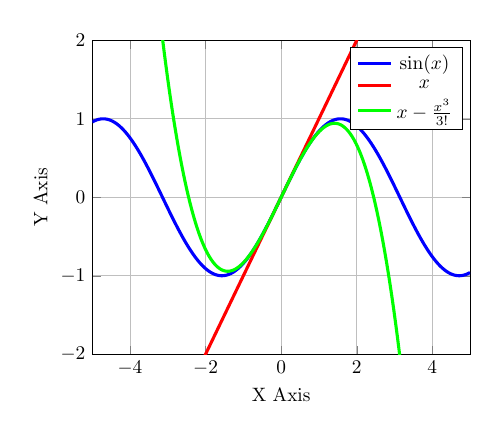
\begin{tikzpicture}[scale=0.7]
			\begin{axis}[
					xmax=5,
					xmin=-5,
					ymax=2,
					ymin=-2,
					samples=1000,
					grid=major,
					xlabel={X Axis},
					ylabel={Y Axis}]
				\addplot[blue, ultra thick,domain=-5:5]{sin(deg(x))};
				\addplot[red, ultra thick,domain=-5:5]{x};
				\addplot[green, ultra thick,domain=-5:5]{x-(x^3/3!)};
				\legend{$\sin(x)$,$x$,$x-\frac{x^3}{3!}$}
			\end{axis}
		\end{tikzpicture}
		\caption{Plot of the Taylor expansion for the function $\sin(x)$}
		\label{sketch:taylor-polynomial:1}
	\end{figure}
\end{exm}

\begin{exm}\label{exm-ln-taylor-series}
	Find the Maclaurin polynomial for the function $f(x)=\ln(x+1)$ of degree $n$.
	\begin{flushleft}
		\textbf{Answer}: Since the Maclaurin polynomial evaluates at $x_0=0$,
		we find that
		\begin{align*}
			 & f(x)=\ln(x+1) \implies f(0)=0                 \\
			 & f'(x)=\frac{1}{x+1} \implies f'(0)=1          \\
			 & f''(x)=-\frac{1}{(x+1)^2} \implies f''(0)=-1  \\
			 & f'''(x)=\frac{2}{(x+1)^3} \implies f'''(0)=-2 \\
		\end{align*}
		After a while it becomes easier to see that there is a pattern to this equation:
		\begin{align*}
			p_n(\ln(x+1),0) & = f(0) + f'(0)x + \frac{f''(0)}{2!}x^2 + \frac{f'''(0)}{3!}x^3 + \cdots + \frac{f^{(n)}(0)}{n!}x^n \\
			                & = x - \frac{x^2}{2} + \frac{x^3}{3} + \cdots + (-1)^{n+1}\frac{x^n}{n}                             \\
			                & = \sum_{k=1}^n (-1)^{k+1}\frac{x^k}{k}
		\end{align*}
	\end{flushleft}
\end{exm}

\begin{thm}\label{thm-taylor-lagrange-remainder-theorem}
	Let $f$ be a $n+1$-times differentiable function in a neighborhood of $x_0$,
	and let $x_0$ be a in that neighborhood. Then by Lagrange's remainder theorem
	there exists a point $\xi$ between $x_0$ and $x$ such that
	\begin{equation}\label{eq-taylor-lagrange-remainder-theorem}
		f(x) = p_n(f,x_0)(x) + \underbrace{\frac{f^{(n+1)}(\xi)}{(n+1)!}(x-x_0)^{n+1}}_{R_n(x)}
	\end{equation}
	where the error incurred by approximating $f$ is denoted by $R_n(x)$ and is
	called the remainder in Lagrange form.
\end{thm}

\begin{rem}
	For $n=0$ we get
	\begin{align*}
		f(x)             & = f(x_0) + f'(\xi)(x-x_0)   \\
		\implies f'(\xi) & = \frac{f(x)-f(x_0)}{x-x_0}
	\end{align*}
	So \hyperref[thm-mean-value-theorem]{the mean value theorem} is a special case
	of Lagrange's remainder theorem.
\end{rem}

\begin{exm}\label{exm-exp-taylor-series}
	The Maclaurin series of the exponential function can be easily found as
	\begin{equation*}
		p_n(\exp(x),0) = \sum_{k=0}^n \frac{x^k}{k!}
	\end{equation*}
	so we can approximate $f(x)=\exp(x)$ with a Taylor polynomial of degree $5$, \textit{i.e.}
	\begin{equation*}
		e^x = p_n(\exp(x),0) + R_n(x)
	\end{equation*}
	Now suppose we require $(\star)$ the remainder in Lagrange form to have at most an
	inaccuracy of $\tfrac{1}{100}$. Then there exists an $0<\xi<1$ and we can roughly
	estimate inaccuracy by
	\begin{align*}
		\abs{R_n(x)} & = \abs[\bigg]{\frac{e^\xi}{(n+1)!}}              \\
		             & = \frac{e^\xi}{(n+1)!}                           \\
		             & < \frac{e}{(n+1)!}                               \\
		             & < \frac{3}{(n+1)!}                               \\
		             & < \frac{1}{100}                     &  & (\star)
	\end{align*}
	Turns out that for $n=5$ the last inequality $(\star)$ holds. In fact, this
	estimation's inaccuracy was already found in the previous step to be $\tfrac{3}{6!}=\tfrac{1}{240}$.
\end{exm}

\begin{thm}\label{thm-infinite-taylor-lagrange-remainder-theorem}
	Let $f$ be a function differentiable infinitely many times in a neighborhood of $x_0$.
	Then there exists a constant $K$ such that for all $n\in\mathbb{N}$,
	\begin{equation}\label{eq-infinite-taylor-lagrange-remainder-theorem}
		\abs{f^{(n)}(x)} \leq K \implies R_n(x) \tolim{n}{\infty} 0
	\end{equation}
\end{thm}


\subsection{Indefinite Integrals}\label{subsec-indefinite-integrals}


\begin{definition}\label{def-indefinite-integral}
	The anti-derivative $F$ of a function $f$ on $I$ is defined such that
	\begin{equation}
		\forall x\in I:  F'(x) = f(x)
	\end{equation}
	When $F$ is an score of anti-derivative of $f$ we denote it by
	\begin{equation}\label{eq-indefinite-integral}
		\int f(x) \diff x = F(x) + C \qquad(C\in\mathbb{R})
	\end{equation}
	where the left-hand side of this equation describes an indefinite integral.
\end{definition}

\begin{exm}\label{exm-indefinite-integral:1}
	Find the indefinite integral of $\sin(x)$ with respect to $x$.
	\begin{flushleft}
		\textbf{Answer}: We can solve the immediate integral using the knowledge
		we obtained during our time when we studied derivatives of functions,
		\textit{i.e.}
		\begin{equation*}
			\int \sin(x) \diff x = -\cos(x) + C
		\end{equation*}
	\end{flushleft}
\end{exm}

\begin{exm}\label{exm-indefinite-integral:2}
	Find the indefinite integral of $x$ with respect to $x$.
	\begin{flushleft}
		\textbf{Answer}:
		\begin{equation*}
			\int x \diff x = -\frac{1}{2}x^2 + C
		\end{equation*}
	\end{flushleft}
\end{exm}

\begin{thm}\label{thm-indefinite-integral-linearity}
	Let $f$ and $g$ be two integrable functions, and let $\lambda\in\mathbb{R}$.
	Then indefinite integral satisfy the linearity property:
	\begin{enumerate}
		\item Addition:
		      \begin{equation}\label{eq-indefinite-integral-linearity:1}
			      \int \left(f(x)+g(x)\right) \diff x = \int f(x) \diff x + \int g(x) \diff x
		      \end{equation}
		\item Multiplication with a scalar:
		      \begin{equation}\label{eq-indefinite-integral-linearity:2}
			      \int \left(\lambda f(x)\right) \diff x = \lambda \int f(x) \diff x
		      \end{equation}
	\end{enumerate}
\end{thm}

\begin{exm}\label{exm-indefinite-integral:3}
	Find the indefinite integral of $\tfrac{x^4}{1+x^2}$ with respect to $x$.
	\begin{flushleft}
		\textbf{Answer}:
		\begin{align*}
			\int \frac{x^4}{1+x^2} \diff x & = \int \frac{x^4-1+1}{1+x^2} \diff x                                                                                \\
			                               & = \int \frac{(x^2-1)(x^2+1)+1}{1+x^2} \diff x                                                                       \\
			                               & = \int (x^2-1) \diff x + \int \frac{1}{1+x^2} \diff x &  & \text{\pref{theorem}{thm-indefinite-integral-linearity}} \\
			                               & = \frac{1}{3}x^3 - x + \arctan(x) + C
		\end{align*}
	\end{flushleft}
\end{exm}

\begin{exm}\label{exm-indefinite-integral:4}
	Find the indefinite integral of $\tan(x)$ with respect to $x$.
	\begin{flushleft}
		\textbf{Answer}: Note, that in general we have that
		\begin{equation}\label{eq-useful-integral}
			\int \frac{f'(x)}{f(x)} \diff x = \ln(\abs{f(x)}) + C \qquad(C\in\mathbb{R})
		\end{equation}
		which can be easily verified by taking the derivative on the right-hand side. Therefore,
		\begin{align*}
			\int \tan(x) \diff x & = \int \frac{\sin(x)}{\cos(x)} \diff x \\
			                     & = -\ln(\abs{\cos(x)}) + C
		\end{align*}
	\end{flushleft}
\end{exm}

\subsubsection{Integration by Parts}\label{subsubsec-integration-by-parts}

\begin{definition}\label{def-integration-by-parts}
	Using integration by parts we can integrate the product of two functions
	$u$,$v$ with respect to $x$ such that
	\begin{align*}
		\underbrace{\int \left(u(x)v(x)\right)' \diff x}_{u(x)v(x)} & = \int u'(x)v(x) \diff x + \int v'(x)u(x) \diff x &  & \text{\pref{definition}{thm-derivative-arithmetic}} \\
		\implies \int v'(x)u(x) \diff x                             & = u(x)v(x) - \int u'(x)v(x) \diff x
	\end{align*}
\end{definition}

\begin{exm}\label{exm-integration-by-parts:1}
	Use integration by parts to find the indefinite integral of $x\exp(x)$ with respect to $x$.
	\begin{flushleft}
		\textbf{Answer}: Let $u(x)=x$ and $v'(x)=\exp(x)$. Then,
		$u'(x)=1$ and $v(x)=\exp(x)$, thus
		\begin{align*}
			\int x\exp(x) \diff x & = x\exp(x) - \int 1\exp(x) \diff x \\
			                      & = \exp(x)\left(x-1\right) + C
		\end{align*}
	\end{flushleft}
\end{exm}

\begin{exm}\label{exm-integration-by-parts:2}
	Use integration by parts to find the indefinite integral of $\exp(x)\cos(x)$ with respect to $x$.
	\begin{flushleft}
		\textbf{Answer}: Let $u(x)=\cos(x)$ and $v'(x)=\exp(x)$. Then,
		$u'(x)=-\sin(x)$ and $v(x)=\exp(x)$, thus
		\begin{align*}
			\int \exp(x)\cos(x) \diff x           & = \exp(x)\cos(x) + \int \exp(x)\sin(x) \diff x                               \\
			                                      & = \exp(x)\cos(x) + \left(\exp(x)\sin(x) - \int \exp(x)\cos(x) \diff x\right) \\
			\implies 2\int \exp(x)\cos(x) \diff x & = \exp(x)\cos(x) + \exp(x)\sin(x) + C                                        \\
			                                      & = \frac{\exp(x)}{2}\big(\cos(x)+\sin(x)\big) + C
		\end{align*}
	\end{flushleft}
\end{exm}

\begin{exm}\label{exm-integration-by-parts:3}
	Use integration by parts to find the indefinite integral of $\arctan(x)$ with respect to $x$.
	\begin{flushleft}
		\textbf{Answer}: Note that $\arctan(x)=1\cdot\arctan(x)$. So, let
		$u(x)=\arctan(x)$ and $v'(x)=1$. Then, $u'(x)=\frac{1}{1+x^2}$ and $v(x)=x$, thus
		\begin{align*}
			\int \arctan(x) \diff x & = x\arctan(x) - \int \frac{x}{1+x^2} \diff x                                                    \\
			                        & = x\arctan(x) - \frac{1}{2}\ln(\abs{1+x^2}) + C &  & \text{\pref{equation}{eq-useful-integral}}
		\end{align*}
	\end{flushleft}
\end{exm}

\begin{exm}\label{exm-integration-by-parts:4}
	Find the indefinite integral of $\exp(-\abs{x})$ with respect to $x$.
	\begin{flushleft}
		\textbf{Answer}:
		\begin{align*}
			\int \exp(-\abs{x}) \diff x & = \begin{cases}
				\int \exp(-x) \diff x \text{ if } x\geq0 \\
				\int \exp(x) \diff x \text{ if } x<0     \\
			\end{cases}                    \\
			                            & \overset{(\star)}{=} \begin{cases}
				-\exp(-x) + 2 + C \text{ if } x\geq0 \\
				\exp(x) + C \text{ if } x<0
			\end{cases}
		\end{align*}
	\end{flushleft}
	Notice that we have to fix the discontinuity in $(\star)$ by adding $2$; see
	also \pref{figure}{sketch:exm-integration-by-parts:4}.
	\begin{equation*}
		\exp(-0)+C_1 = \exp(0) + C_2  \implies C_1 = 2 + C_2
	\end{equation*}
	If it weren't for this
	change the function would no longer be continuous (and by extension differentiable
	at $x=0$, \textit{cf.} \pref{remark}{rem-continuity-doesnt-imply-differentiability}),
	which in turn would violate \pref{definition}{def-indefinite-integral}.
	\begin{flushleft}
		\textbf{Left-hand side limit at $x=0$}:
		\begin{align*}
			F_-'(x_0) & = \lim_{h\to0^+}\frac{F(x_0+h)-F(x_0)}{h}                                                              \\
			          & = \lim_{h\to0^+}\frac{\exp(x_0+h)+C-(-\exp(-x_0)+2+C)}{h}                                              \\
			          & = \lim_{h\to0^+}\frac{\exp(x_0)\exp(h)+\exp(x_0)-2}{h}    &  & x_0 = 0                                 \\
			          & = \lim_{h\to0^+}\frac{\exp(h)-1}{h}                       &  & \text{\pref{definition}{def-euler-alt}} \\
			          & = 1
		\end{align*}
		\textbf{Right-hand side limit at $x=0$}:
		\begin{align*}
			F_+'(x_0) & = \lim_{h\to0^-}\frac{F(x_0+h)-F(x_0)}{h}                                                                 \\
			          & = \lim_{h\to0^-}\frac{\exp(-x_0-h)+2+C-(-\exp(-x_0)+2+C)}{h} &  & x_0 = 0                                 \\
			          & = \lim_{h\to0^-}\frac{-\exp(h)+1}{h}                         &  & \text{\pref{definition}{def-euler-alt}} \\
			          & = 1
		\end{align*}
	\end{flushleft}
	\begin{figure}[ht!]
		\centering
		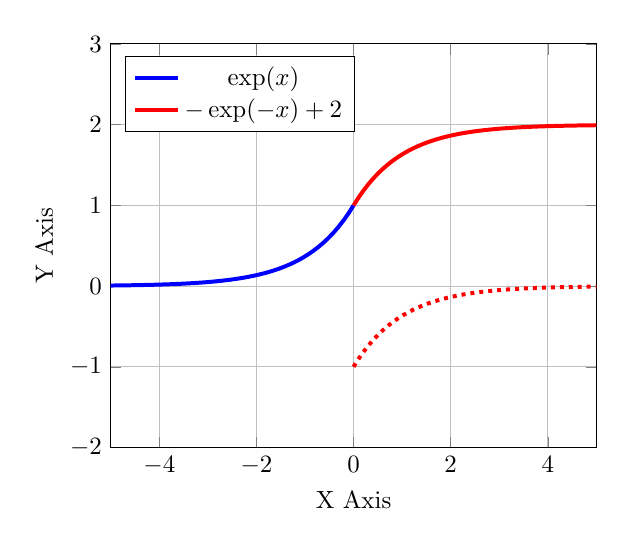
\begin{tikzpicture}[scale=0.9]
			\begin{axis}[
					xmax=5,
					xmin=-5,
					ymax=3,
					ymin=-2,
					samples=50,
					grid=major,
					xlabel={X Axis},
					ylabel={Y Axis},
					legend pos=north west
				]
				\addplot[blue,ultra thick,domain=-5:0]{exp(x)};
				\addplot[red,ultra thick,domain=0:5]{-exp(-x)+2};
				\addplot[red,ultra thick,dotted,domain=0:5]{-exp(-x)};
				\legend{$\exp(x)$,$-\exp(-x)+2$}
			\end{axis}
		\end{tikzpicture}
		\caption{Plot of the indefinite integral of $\exp(-\abs{x})$}
		\label{sketch:exm-integration-by-parts:4}
	\end{figure}
\end{exm}

\subsubsection{Integration of Rational Functions}\label{subsubsec-integration-rational-functions}

\begin{flushleft}
	Rational functions are of the form $\tfrac{p(x)}{q(x)}$ (where $p(x)$ and $q(x)$
	are polynomials and $q(x)\neq0$) that require different approaches when it
	comes to integration depending on the situation at hand. In this subsection
	we will walk through each case step by step by example, rather than proving
	the theorem that provides the underlying theory.
\end{flushleft}

\begin{exm}\label{exm-integration-rational-function:1}
	Find the indefinite integral of
	\begin{equation*}
		\int \frac{2x^4-x^3-x^2+3x-4}{x^2+1} \diff x
	\end{equation*}
	\begin{flushleft}
		\textbf{Answer}: In this example we have to first simplify the expression
		algebraically by performing a long division with polynomials\footnote{See
			also: \url{https://en.wikipedia.org/wiki/Polynomial_long_division}}, the
		result of which is
		\begin{align*}
			\int \frac{2x^4-x^3-x^2+3x-4}{x^2+1} \diff x
			 & = \int \left(2x^2-x-3+\frac{4x-1}{x^2-1}\right) \diff x                                                                                       \\
			 & = \frac{2}{3}x^3 -\frac{1}{2}x^2-3x + \int \frac{4x-1}{x^2-1} \diff x         &  & \text{\pref{example}{exm-integration-rational-function:4}} \\
			 & = \frac{2}{3}x^3 -\frac{1}{2}x^2-3x + \ln(\abs{3x-1}) + \frac{2}{3(3x-1)} + C
		\end{align*}
		\textit{This kind of situation occurs when $\deg(p)>\deg(q)$.}
	\end{flushleft}
\end{exm}

\begin{exm}\label{exm-integration-rational-function:2}
	Find the indefinite integral of
	\begin{equation*}
		\int \frac{1}{2x^2+9x-5} \diff x
	\end{equation*}
	\begin{flushleft}
		\textbf{Answer}: In this example we use \gls{pfd} to split up the integral
		into two parts\footnote{See also: \url{https://en.wikipedia.org/wiki/Partial_fraction_decomposition}}
		\begin{align*}
			\int \frac{1}{2x^2+9x-5} \diff x
			 & = \int \frac{1}{(2x-1)(x+5)} \diff x                                                                                              \\
			 & = \int \frac{A}{2x-1} \diff x + \int \frac{B}{x+5} \diff x                                                                        \\
			 & = \int \frac{\frac{2}{11}}{2x-1} \diff x + \int \frac{-\frac{1}{11}}{x+5} \diff x                                                 \\
			 & = \frac{1}{11}\int \frac{2}{2x-1} - \frac{1}{11} \int \frac{1}{x+5} \diff x       &  & \text{\pref{equation}{eq-useful-integral}} \\
			 & = \frac{1}{11}\ln(\abs{2x-1}) - \frac{1}{11}\ln(\abs{x+5}) + C
		\end{align*}
		\textit{This kind of situation occurs when the denominator $q$ has distinct
			linear factors.}
	\end{flushleft}
\end{exm}

\begin{exm}\label{exm-integration-rational-function:3}
	Find the indefinite integral of
	\begin{equation*}
		\int \frac{9x-5}{9x^2-6x+1} \diff x
	\end{equation*}
	\begin{flushleft}
		\textbf{Answer}: This type of integral is similar to the one we encountered
		in \pref{example}{exm-integration-rational-function:1}, but it has a little
		twist to it as can be observed in the solution below:
		\begin{align*}
			\int \frac{9x-5}{9x^2-6x+1} \diff x
			 & = \int \frac{9x-5}{(3x-1)^2} \diff x                                                                            \\
			 & = \int \frac{A}{3x-1} \diff x + \int \frac{B}{(3x-1)^2} \diff x                                                 \\
			 & = \int \frac{3}{3x-1} \diff x - \int \frac{2}{(3x-1)^2} \diff x &  & \text{\pref{equation}{eq-useful-integral}} \\
			 & = \ln(\abs{3x-1}) + \frac{2}{3}\cdot\frac{1}{3x-1} + C
		\end{align*}
		\textit{This kind of situation occurs when $q$ has a linear factor with
			multiplicity greater than or equal to $2$.}
	\end{flushleft}
\end{exm}

\begin{exm}\label{exm-integration-rational-function:4}
	Find the indefinite integral of
	\begin{equation*}
		\int \frac{4x-1}{x^2-1} \diff x
	\end{equation*}
	\begin{flushleft}
		\textbf{Answer}: This one is kind of weird, but it turns out to be not as
		involved as the previous examples once we recognize that we can force this
		integral into a form that is easier to solve:
		\begin{align*}
			\int \frac{4x-1}{x^2-1} \diff x
			 & = 2 \int \frac{2x}{x^2-1} \diff x - \int \frac{1}{x^2-1} \diff x &  & \text{\pref{equation}{eq-useful-integral}} \\
			 & = 2\ln(\abs{x^2-1}) - \arctan(x) + C
		\end{align*}
		\textit{This kind of situation occurs when $q$ has a quadratic irreducible
			factor does not break into linear factors.}
	\end{flushleft}
\end{exm}

\begin{exm}\label{exm-integration-rational-function:5}
	Find the indefinite integral of
	\begin{equation*}
		\int \frac{1}{x^2-x-1} \diff x
	\end{equation*}
	\begin{flushleft}
		\textbf{Answer}: This type of integral is of the set of problems as
		\pref{example}{exm-integration-rational-function:4}, but here we use a
		different approach: We use the identity
		\begin{equation}\label{eq-useful-square-identity}
			x^2 + px + q = \left(x+\frac{p}{2}\right)^2 + \left(q - \frac{p^2}{4}\right)
		\end{equation}
		So, the integral simplifies to
		\begin{align*}
			\int \frac{1}{x^2-x-1} \diff x
			 & = \int \frac{1}{\left(x-\frac{1}{2}\right)^2+\frac{3}{4}} \diff x                                           &  & \text{\pref{equation}{eq-useful-square-identity}} \\
			 & = \frac{4}{3} \int \frac{1}{\left(\frac{2}{\sqrt{3}}\left(x-\frac{1}{2}\right)\right)^2+1} \diff x                                                                 \\
			 & = \frac{4}{3} \cdot \frac{\sqrt{3}}{2} \arctan\left(\frac{2}{\sqrt{3}}\left(x-\frac{1}{2}\right)\right) + C                                                        \\
			 & = \frac{2\sqrt{3}}{3} \arctan\left(\frac{2}{\sqrt{3}}\left(x-\frac{1}{2}\right)\right) + C                                                                         \\
		\end{align*}
		\textit{This kind of situation occurs when $q$ has a quadratic irreducible
			factor does not break into linear factors.}
	\end{flushleft}
\end{exm}

\begin{exm}\label{exm-integration-rational-function:6}
	Find the indefinite integral of
	\begin{equation*}
		\int \frac{-x+2}{x^2-x+1} \diff x
	\end{equation*}
	\begin{flushleft}
		\textbf{Answer}: In this example we are still exploring the situation
		has a quadratic irreducible factor does not break into linear factors.
		\begin{align*}
			\int \frac{-x+2}{x^2-x+1} \diff x
			 & = -\frac{1}{2} \int \frac{2x-1}{x^2-x+1} \diff x + \frac{3}{2}\int \frac{1}{x^2-x+1} \diff x                      &  & \text{\pref{example}{exm-integration-rational-function:5}} \\
			 & = -\frac{1}{2}\ln(\abs{x^2-x-+1}) + \sqrt{3} \arctan\left(\frac{2}{\sqrt{3}}\left(x-\frac{1}{2}\right)\right) + C
		\end{align*}
		\textit{This kind of situation occurs when $q$ has a quadratic irreducible
			factor does not break into linear factors.}
	\end{flushleft}
\end{exm}

\begin{exm}\label{exm-integration-rational-function:7}
	Find the indefinite integral of
	\begin{equation*}
		\int \frac{1}{x^3+1} \diff x
	\end{equation*}
	\begin{flushleft}
		\textbf{Answer}: Finding the roots of polynomials of degree $3$ or higher is
		usually rather difficult, but in this example we can already see that $-1$ is
		a root of this polynomial. Therefore, we are in a position where we can use
		\gls{pfd} again to solve this integral:
		\begin{align*}
			\int \frac{1}{x^3+1} \diff x
			 & = \int \frac{1}{(x+1)(x^2-x=1)} \diff x                                                                                                                         \\
			 & = \int \frac{A}{x+1} \diff x + \int \frac{Bx+C}{x^2-x+1} \diff x                                                                                                \\
			 & = \int \frac{\frac{1}{3}}{x+1} \diff x + \int \frac{-\frac{1}{3}x+\frac{2}{3}}{x^2-x+1} \diff x                                                                 \\
			 & = \frac{1}{3} \frac{1}{x+1} \diff x + \frac{1}{3} \int \frac{-x+2}{x^2-x+1} \diff x             &  & \text{\pref{example}{exm-integration-rational-function:6}} \\
			 & = \frac{1}{3}\ln(\abs{x+1}) -\frac{1}{6}\ln(\abs{x^2-x-+1})                                                                                                     \\
			 & + \frac{1}{\sqrt{3}} \arctan\left(\frac{2}{\sqrt{3}}\left(x-\frac{1}{2}\right)\right) + C
		\end{align*}
		\textit{This kind of situation occurs when $\deg(q)=3$.}
	\end{flushleft}
\end{exm}

\subsubsection{Integration by Substitution}\label{subsubsec-integration-by-substitution}

\begin{thm}\label{thm-integration-using-substitution}
	If $x=\varphi(u)$ is differentiable and invertible, then the formula for
	substitution\footnote{Sometimes also called change of variables} is
	\begin{equation}\label{eq-integration-using-substitution}
		\int f(x) \diff x = \int f(\varphi(u))\varphi'(u) \diff u
	\end{equation}
\end{thm}

\begin{exm}\label{exm-integration-using-substitution:1}
	Use the substitution technique to find the indefinite integral of $\arctan(x)$ with respect to $x$.
	\begin{flushleft}
		\textbf{Answer}: Let $u \defines \exp(x)$. Then $\diff u = \exp(x) \diff x$, and
		\begin{align*}
			\int \frac{\exp(x)}{\exp(2x)+1} \diff x & = \int \frac{1}{u^2+1} \diff u \\
			                                        & = \arctan(\abs{u}) + C         \\
			                                        & = \arctan(\abs{\exp(x)}) + C
		\end{align*}
	\end{flushleft}
\end{exm}

\begin{exm}\label{exm-integration-using-substitution:2}
	Use the substitution technique to find the indefinite integral of $2x\exp(x^2)$ with respect to $x$.
	\begin{flushleft}
		\textbf{Answer}: Let $u \defines x^2$. Then $\diff u = 2x \diff x$, and
		\begin{align*}
			\int 2x\exp(x^2) \diff x & = \int \exp(u) \diff u \\
			                         & = \exp(u) + C          \\
			                         & = \exp(x^2) + C
		\end{align*}
	\end{flushleft}
\end{exm}

\begin{exm}\label{exm-integration-using-substitution:3}
	Use the substitution technique to find the indefinite integral of $\tfrac{\sqrt{x}}{x+1}$ with respect to $x$.
	\begin{flushleft}
		\textbf{Answer}: Let $u \defines \sqrt{x}$. Then $x = u^2$ and $\diff x = 2u \diff u$, so
		\begin{align*}
			\int \frac{\sqrt{x}}{x+1} \diff & = 2\int \frac{u^2+1-1}{u^2+1} \diff u                          \\
			                                & = 2 \left(\int 1 \diff u - \int \frac{1}{u^2+1} \diff u\right) \\
			                                & = 2u - 2\arctan(\abs{u}) + C                                   \\
			                                & = 2\sqrt{x} - 2\arctan(\sqrt{x}) + C
		\end{align*}
	\end{flushleft}
\end{exm}

\begin{exm}\label{exm-integration-using-substitution:4}
	Use the substitution technique to find the indefinite integral of $\tfrac{1}{\cos(x)}$ with respect to $x$.
	\begin{flushleft}
		\textbf{Answer}: Let $u \defines \tan\left(\tfrac{x}{2}\right)$. Then $x = 2\arctan(u)$
		and $\diff x = \tfrac{2}{1+u^2} \diff u$. Note that $u=\sqrt{\frac{1-\cos(x)}{1+\cos(x)}}$, so
		\begin{align*}
			u^2                       & = \frac{1-\cos(x)}{1+\cos(x)} \\
			\implies u^2 + u^2\cos(x) & = 1 - \cos(x)                 \\
			\implies \cos(x)          & = \frac{1-u^2}{1+u^2}
		\end{align*}
		Therefore the integral becomes
		\begin{align*}
			\int \frac{1}{\cos(x)} \diff x & = \int \frac{1+u^2}{1-u^2} \cdot \frac{2}{1+u^2} \diff u                                                  \\
			                               & = \int \frac{2}{1-u^2} \diff u                                                                            \\
			                               & = \int \frac{1}{1-u} \diff u + \int \frac{1}{1+u} \diff u                                                 \\
			                               & = -\ln(\abs{1-u}) + \ln(\abs{1+u}) + C                                                                    \\
			                               & = -\ln\left(\abs[\Bigg]{\frac{1+\tan\left(\frac{x}{2}\right)}{1-\tan\left(\frac{x}{2}\right)}}\right) + C \\
		\end{align*}
	\end{flushleft}
\end{exm}


\subsection{Definite Integrals}\label{subsec-definite-integrals}

\begin{definition}\label{def-partition-of-an-interval}
	A partition of an interval $[a,b]$ on $\mathbb{R}$ is a finite sequence
	$x_0,x_1,\dots,x_n$ of real numbers such that
	\begin{equation}\label{eq-partition-of-an-interval}
		a = x_0 < x_1 < \dots < x_n = b
	\end{equation}
	and is denoted by $P$.
\end{definition}

\begin{definition}\label{def-max-partition}
	The biggest interval of the partition is defined by
	\begin{equation}\label{eq-max-partition}
		\lambda(P) \defines \max\left\{\Delta x_i \setbuild i\in\mathbb{N}\right\}
	\end{equation}
\end{definition}

\begin{definition}\label{def-riemann-sum}
	Let $P$ be a partition of $[a,b]$, and let $f:[a,b]\to\mathbb{R}$ be bounded.
	Choose points $x_i^*\in[x_{i-1},x_i]$ for $i\in\mathbb{N}$. Then
	\begin{equation}\label{eq-riemann-sum}
		\sum_{i=1}^n f(x_i^*)(x_i-x_{i-1}) = \sum_{i=1}^n f(x_i^*)\Delta x
	\end{equation}
	is called the Riemann sum for $f$ determined by the partition $P$.
\end{definition}

\begin{definition}\label{def-riemann-integrable}
	Let $f:[a,b]\to\mathbb{R}$ be bounded. We say that $f$ is a Riemann integrable
	function on $[a,b]$ if there exists an $I\in\mathbb{R}$ such that
	\begin{equation}
		\bigwedge_{\varepsilon>0}\bigvee_{\delta>0}\bigwedge_{\lambda(P)<\delta}
		\abs[\Bigg]{\sum_{i=1}^n f(x_i^*)\Delta x_i - I}<\varepsilon
	\end{equation}
	for all $x_i^*$.
\end{definition}

\begin{definition}\label{def-definite-integral}
	For a continuous function and bounded function $f:[a,b]\to\mathbb{R}$,
	the Riemann sum can by computed by
	\begin{equation}\label{eq-definite-integral}
		\int_a^b f(x) \diff x = \lim_{n\to\infty}\sum_{i=1}^n f(x_i^*)\Delta x
	\end{equation}
	for any choice of the $x_i^*\in[x_{i-1},x_i]$ with $\delta x = \tfrac{b-a}{n}$
	and $x_i = a + (i-1)\Delta x_i$, \textit{i.e.} $P$ partitions the interval $[a,b]$
	into subintervals of equal length\footnote{which are also called regular intervals}.
\end{definition}

\begin{rem}\label{rem-definite-integral}
	To determine the value of $x_i$, we use the formula
	\begin{enumerate}
		\item Left-Hand Rule: $\sum_{i=1}^n f(x_i)\Delta x$
		\item Midpoint Rule: $\sum_{i=1}^n f(x_{i+1})\Delta x$
		\item Right-Hand Rule: $\sum_{i=1}^n f\left(\frac{x_i+x_{i+1}}{2}\right)\Delta x$
	\end{enumerate}
\end{rem}

\begin{exm}\label{exm-riemann-sum:1}
	Consider the constant function $f(x)=c$ on the interval $[a,b]$. For any $P$
	and choice off $c_i$ we get
	\begin{align*}
		\sum_{i=1}^n c \Delta x & = c \sum_{i=1}^n \Delta x \\
		                        & = c (b-a)
	\end{align*}
	Hence,
	\begin{equation*}
		\int_a^b c \diff x = c(b-a)
	\end{equation*}
\end{exm}

\begin{exm}\label{exm-riemann-sum:2}
	Consider the linear function $f(x)=x$ on the interval $[0,1]$. For any $P$
	and choice off $c_i$ we partition the interval into subintervals of length $n$
	using the right-hand rule, so $\Delta x = \frac{1}{n}$, and
	\begin{equation*}
		x_i = 0 + ((i+1)-1)\Delta x = \frac{i}{n}
	\end{equation*}
	Then the Riemann sum of this function is
	\begin{align*}
		\sum_{i=1}^n f(x_{i+1}) \Delta x & = \sum_{i=1}^n f\left(\frac{i}{n}\right)\Delta x \\
		                                 & = \frac{1}{n^2} \sum_{i=1}^n i                   \\
		                                 & = \frac{1}{n^2} \cdot \frac{n(n+1)}{2}           \\
		                                 & = \frac{n+1}{2n}
	\end{align*}
	Hence,
	\begin{equation*}
		\int_0^1 x \diff x = \lim_{n\to\infty}\frac{n+1}{2n} = \frac{1}{2}
	\end{equation*}
\end{exm}

\begin{exm}\label{exm-riemann-sum:3}
	Compute the Riemann sum of $f(x)=4x-x^2$ on $[0,4]$ with regular partitions
	$16$ using the left and right-hand rule from \pref{remark}{rem-definite-integral}.
	\begin{flushleft}
		\textbf{Answer}: Note that $a=0$ and $b=4$. From \pref{definition}{def-definite-integral}
		we have that for the right-hand rule,
		\begin{align*}
			\Delta x & = \frac{4-0}{16} = \frac{1}{4}      \\
			x_i      & = 0 + ((i+1)-1)\Delta x = i\Delta x
		\end{align*}
		Using the left-hand rule we get
		\begin{align*}
			\sum_{i=1}^{16} f(x_{i+1})\Delta x & = \sum_{i=1}^{16} f(i\Delta x)\Delta x                               \\
			                                   & = \sum_{i=1}^{16} \left(4 i \Delta x - i^2 \Delta x^2\right)\Delta x \\
			                                   & = 4 \Delta x^2 \sum_{i=1}^{16} i - \Delta x^3 \sum_{i=1}^{16} i^2    \\
			                                   & = 10.625
		\end{align*}
	\end{flushleft}
\end{exm}

\begin{rem}
	If $I\defines \int_a^b f(x) \diff x$ in \pref{definition}{def-definite-integral}
	exists, then it is unique.
\end{rem}

\begin{definition}\label{def-definite-integral-properties}
	The following properties of the definite integral can be deduced from the
	Riemann sum approach to integration:
	\begin{enumerate}
		\item Additive properties:
		      \begin{align}
			      \int_a^c f(x) \diff x & = \int_a^b f(x) \diff x + \int_b^c f(x) \diff x \\
			      \int_a^a f(x) \diff x & = 0                                             \\
			      \int_a^b f(x) \diff x & = -\int_b^a f(x) \diff x
		      \end{align}
	\end{enumerate}
\end{definition}

\begin{thm}\label{thm-continuous-monotone-integrable}
	If $f$ is piecewise continuous or piecewise monotone, then $f$ is (Riemann)
	integrable.
\end{thm}

\begin{thm}\label{thm-definite-integral-theorems}
	Let $f:[a,b]\to\mathbb{R}$ be a bounded function.
	\begin{enumerate}
		\item If $f$ is integrable on $[a,b]$, then it is integrable on any $[c,d]\subseteq[a,b]$.
		\item If $f$ and $g$ are integrable on $[a,b]$ and $\alpha,\beta\in\mathbb{R}$, then $\alpha f(x)+ \beta g(x)$ is integrable, and
		      \begin{equation}\label{eq-definite-integral-linearity}
			      \int_a^b \left(\alpha f(x)+ \beta g(x)\right) \diff x = \alpha \int_a^b f(x) \diff x + \beta \int_a^b g(x) \diff x
		      \end{equation}
		\item If $f$ and $g$ are integrable on $[a,b]$, then $(f \circ g)(x)$ is also integrable.
		\item If $f$ is integrable on $[a,b]$, then so is $\abs{f}$, and the following inequality holds:
		      \begin{equation}\label{eq-definite-integral-triangle-inequality}
			      \abs[\Bigg]{\int_a^b f(x) \diff x} \leq \int_a^b \abs{f(x)} \diff x
		      \end{equation}
		\item If $f$ is integrable on $[a,b]$ and $f(x)\geq0$ for every $x\in\domain{f}$, then\footnote{If $f(x_0)>0$ for some $x_0$,
			      $\int_a^b f(x) \diff x$ need not to strictly greater than zero. However, one can correct this by demanding continuity for $f$.}
		      \begin{equation}\label{eq-definite-integral-positvity}
			      \int_a^b f(x) \diff x \geq 0
		      \end{equation}
		\item If $f$ and $g$ are integrable on $[a,b]$ and $f(x)\geq g(x)$ for all $x\in\domain{f}$, then
		      \begin{equation}\label{eq-definite-integral-monotonicity}
			      \int_a^b f(x) \diff x \geq \int_a^b g(x) \diff x
		      \end{equation}
		\item If $f$ is integrable on $[a,b]$ and $m \leq f(x) \leq M$ for all $x\in\domain{f}$, then
		      \begin{equation}\label{eq-definite-integral-bounded}
			      m(b-a) \leq \int_a^b f(x) \diff x \leq M(b-a)
		      \end{equation}
		\item If $f$ is integrable on $[a,b]$ and continuous, there exists a $c\in[a,b]$ such that
		      \footnote{This is also called the intermediate value theorem for integrals, \textit{cf.} \pref{theorem}{thm-intermediate-value-theorem}}
		      \begin{equation}\label{eq-intermediate-value-theorem-for-theorems}
			      \int_a^b f(x) \diff x = f(c)(b-a)
		      \end{equation}
		\item If $f$ is integrable on $[a,b]$ and $\tilde{f}$ differs from $f$ at finitely many points, then $\tilde{f}$ is integrable and
		      \begin{equation}\label{eq-change-points-retain-integral}
			      \int_a^b f(x) \diff x =  \int_a^b \tilde{f}(x) \diff x
		      \end{equation}
	\end{enumerate}
\end{thm}

\begin{proof}
	Of \pref{equation}{eq-intermediate-value-theorem-for-theorems} in \pref{theorem}{thm-definite-integral-theorems}.
	\begin{flushleft}
		By \pref{equation}{eq-definite-integral-bounded} we know that
		\begin{equation*}
			m(b-a) \leq \int_a^b f(x) \diff x \leq M(b-a)
		\end{equation*}
		Then this implies
		\begin{align*}
			m \leq \frac{1}{b-a}\int_a^b f(x) \diff x \leq M
		\end{align*}
		So, by the intermediate value \pref{theorem}{thm-intermediate-value-theorem},
		there exists a $c$ such that
		\begin{equation*}
			f(c) =  \frac{1}{b-a}\int_a^b f(x) \diff x
		\end{equation*}
	\end{flushleft}
\end{proof}

\begin{thm}\label{thm-integrable-continuous}
	If $f$ is integrable on $[a,b]$, then
	\begin{equation}
		F(x) = \int_a^x f(t) \diff t
	\end{equation}
	is continuous on $[a,b]$.
\end{thm}

\subsubsection{The Fundamental Theorem of Calculus}\label{subsubsec-the-fundamental-theorem-of-calculus}

\begin{thm}\label{thm-the-fundamental-theorem-of-calculus}
	Suppose that $f:[a,b]\to\mathbb{R}$ is continuous. Define
	\begin{equation*}
		F(x) = \int_a^x f(t) \diff t
	\end{equation*}
	Then $F$ is differentiable. Moreover,
	\begin{equation}
		F'(x) = f(x)
	\end{equation}
\end{thm}

\begin{proof}
	Of \pref{theorem}{thm-the-fundamental-theorem-of-calculus}.
	\begin{flushleft}
		For any $x_0\in[a,b]$,
		\begin{align*}
			F_+'(x_0) & = \lim_{x \to x_0^+} \frac{F(x)-F(x_0)}{x-x_0}                                       &  & \text{\pref{theorem}{thm-integrable-continuous}}                   \\
			          & = \lim_{x \to x_0^+} \frac{\int_a^x f(t) \diff t - \int_a^{x_0} f(t) \diff t}{x-x_0}                                                                         \\
			          & = \lim_{x \to x_0^+} \frac{\int_{x_0}^x f(t) \diff t}{x-x_0}                         &  & \text{\pref{equation}{eq-intermediate-value-theorem-for-theorems}} \\
			          & = \lim_{x \to x_0^+} \frac{f(c_x)(x-x_0)}{x-x_0}                                                                                                             \\
			          & = \lim_{x \to x_0^+} f(c_x)                                                          &  & \text{\pref{definition}{def-continuity-at-point-a}}                \\
			          & = f(x_0)
		\end{align*}
	\end{flushleft}
\end{proof}

\begin{crl}\label{crl-continuity-implies-anti-derivative}
	Every continuous function has an anti-derivative.
\end{crl}

\begin{rem}\label{rem-continuity-implies-anti-derivative}
	Although the anti-derivative is not always an elementary function.
\end{rem}

\begin{crl}\label{crl-newton-leibniz-formula}
	Let $f:[a,b]\to\mathbb{R}$ be continuous and let $F(x)$ be an anti-derivative
	of $f$. Then
	\begin{equation}\label{eq-newton-leibniz-formula}
		\int_a^b f(x) \diff x = F(b) - F(a) = \evalat{F}{a}{b}
	\end{equation}
\end{crl}

\begin{exm}\label{exm-newton-leibniz-formula:1}
	Find the definite integral of
	\begin{equation*}
		f(x) = 2 + \cos(x) - \frac{x^2}{2}
	\end{equation*}
	from $0$ to $\tfrac{\pi}{2}$ with respect to $x$.
	\begin{flushleft}
		\textbf{Answer}:
		\begin{align*}
			\int_0^{\frac{\pi}{2}} f(x) \diff x & = \evalat{\left(2x+\sin(x)-\frac{x^3}{3}\right)}{0}{\frac{\pi}{2}}                                       \\
			                                    & = \left(2\cdot\frac{\pi}{2}+\sin\left(\frac{\pi}{2}\right)-\frac{\left(\frac{\pi}{2}\right)^3}{3}\right)
			- \left(2\cdot0+\sin(0)-\frac{0^3}{3}\right)                                                                                                   \\
			                                    & = \pi+1-\frac{\pi^3}{24}
		\end{align*}
	\end{flushleft}
\end{exm}

\begin{proof}
	Of \pref{corollary}{crl-newton-leibniz-formula}.
	\begin{flushleft}
		Define $G(x)=\int_a^x f(t) \diff t$. By \pref{theorem}{thm-the-fundamental-theorem-of-calculus},
		$G'(x)=f(x)$. Hence, there exists a constant $C\in\mathbb{R}$ such that $F(x)=G(x)+C$.
		Therefore,
		\begin{align*}
			F(b) - F(a) & = (G(b)+c) - (G(a)+c)                                                                                           \\
			            & = G(b) - G(a)                                                                                                   \\
			            & = \int_a^b f(x) \diff x - \int_a^a f(x) \diff x &  & \text{\pref{definition}{def-definite-integral-properties}} \\
			            & = \int_a^b f(x) \diff x
		\end{align*}
	\end{flushleft}
\end{proof}

\begin{exm}\label{exm-newton-leibniz-formula:2}
	Evaluate the following expression:
	\begin{equation*}
		\lim_{x\to0}\frac{1}{x^3}\int_0^x \sin^2(3t) \diff t
	\end{equation*}
	\begin{flushleft}
		\textbf{Answer}:
		\begin{align*}
			\lim_{x\to0}\frac{1}{x^3}\int_0^x \sin^2(3t) \diff t
			 & = \lim_{x\to0}\frac{\int_0^x \sin^2(3t) \diff t}{x^3} &  & \text{\pref{theorem}{thm-lhopitals-rule}, (\ref{thm-the-fundamental-theorem-of-calculus})} \\
			 & = \lim_{x\to0}\frac{3\sin^2(3x)}{3\cdot3x^2}          &  & \text{\pref{equation}{eq-important-sin-over-x-limit}}                                      \\
			 & = 1
		\end{align*}
	\end{flushleft}
\end{exm}

\begin{exm}\label{exm-newton-leibniz-formula:3}
	Let $G(x)=\int_0^{x+x^2}\sin(t)\diff t$. Find the first derivative of $G$.
	\begin{flushleft}
		\textbf{Answer}: By \pref{theorem}{thm-the-fundamental-theorem-of-calculus},
		that
		\begin{equation*}
			F(x)=\int_0^{x}\sin(t)\diff t \implies G'(x) = \sin(x)
		\end{equation*}
		Note that $G(x)=F(x+x^2)$, so
		\begin{align*}
			G'(x) & = F'(x+x^2)(1+2x)   \\
			      & = \sin(x+x^2)(1+2x)
		\end{align*}
	\end{flushleft}
\end{exm}

\begin{rem}\label{rem-newton-leibniz-formula}
	The implication below makes sense when $f$ is continuous, but when we drop this
	condition we will suddenly see that there are integrable function that are not
	continuous - take, for instance, the function
	\begin{equation*}
		f(x) = \begin{cases}
			1\text{ if } x\geq0 \\
			0\text{ else }
		\end{cases}
	\end{equation*}
	Obviously, $f(x)$ is piecewise integrable because it is piecewise continuous,
	but it doesn't have an anti-derivative on the entire interval since it has a
	jump discontinuity in the origin. So, it is not continuous at $x=0$ which
	violates \pref{definition}{def-indefinite-integral}. Therefore, in general
	\begin{equation}\label{eq-rem-newton-leibniz-formula:ltr}
		\text{$f$ is integrable} \notimplies \text{$f$ has an anti-derivative}
	\end{equation}
	Conversely, the other direction also doesn't hold:
	\begin{equation}\label{eq-rem-newton-leibniz-formula:rtl}
		\text{$f$ has an anti-derivative} \notimplies \text{$f$ is integrable}
	\end{equation}
	A function can be unbounded but still have an anti-derivative; but if the
	function is not bounded, then it is not integrable. For example, the function
	\begin{equation*}
		f:(0,1)\to\mathbb{R},x\mapsto\frac{1}{x}
	\end{equation*}
	is not bounded, which is why it is not integrable. This is the reason why we
	demand continuity in the fundamental theorem of \pref{calculus}{thm-the-fundamental-theorem-of-calculus}.
\end{rem}

\subsubsection{Integration by Parts}\label{subsubsec-integration-by-parts-definite-integrals}

\begin{thm}\label{thm-integration-by-parts-definite-integrals}
	If $u(x)$ and $v(x)$ have continuous derivatives on $[a,b]$ (\textit{cf.}
	\pref{definition}{def-integration-by-parts}), then
	\begin{equation}\label{eq-integration-by-parts-definite-integrals}
		\int_a^b u(x) v'(x) \diff x = \evalat{u(x)v(x)}{a}{b} - \int_a^b u'(x) v(x) \diff x
	\end{equation}
\end{thm}

\begin{proof}
	Of \pref{theorem}{thm-integration-by-parts-definite-integrals}.
	\begin{flushleft}
		From the product rule in \pref{theorem}{thm-derivative-arithmetic} we know that
		\begin{equation*}
			(u(x)v(x))' = u(x)v'(x) + u'(x)v(x)
		\end{equation*}
		So, because the derivatives are continuous we can write
		\begin{align*}
			\int_a^b (u(x)v(x))' \diff x & = \int_a^b u(x)v'(x) \diff x + \int_a^b u'(x)v(x) \diff x                                                          \\
			\implies
			\evalat{u(x)v(x)}{a}{b}      & = \int_a^b u(x)v'(x) \diff x + \int_a^b u'(x)v(x) \diff x &  & \text{\pref{corollary}{crl-newton-leibniz-formula}} \\
			\implies
			\int_a^b u(x)v'(x) \diff x   & = \evalat{u(x)v(x)}{a}{b} -  \int_a^b u'(x)v(x) \diff x
		\end{align*}
	\end{flushleft}
\end{proof}

\begin{exm}\label{exm-integration-by-parts-definite-integrals}
	Find the definite integral of
	\begin{equation*}
		f(x) = x\sin(x)
	\end{equation*}
	from $0$ to $\pi$ with respect to $x$.
	\begin{flushleft}
		\textbf{Answer}: Let $u(x)=x$ and $v'(x)=\sin(x)$. Then by
		\pref{theorem}{thm-integration-by-parts-definite-integrals}), (with $u'(x)=1$
		and $v(x)=-\cos(x)$) it follows that
		\begin{align*}
			\int_0^\pi x\sin(x) \diff x & = \evalat{-x\cos(x)}{0}{\pi} + \int_0^\pi \cos(x) \diff x                                                          \\
			                            & = \pi - \evalat{\sin(x)}{0}{\pi}                          &  & \text{\pref{corollary}{crl-newton-leibniz-formula}} \\
			                            & = \pi
		\end{align*}
	\end{flushleft}
\end{exm}

\begin{rem}
	So there are two methods to solve definite integrals:
	\begin{enumerate}
		\item[a)] Find an anti-derivative and then use \pref{corollary}{crl-newton-leibniz-formula}
		\item[b)] Only use theorems for definite integral to simplify the expression and then use \pref{corollary}{crl-newton-leibniz-formula}
	\end{enumerate}
\end{rem}

\subsubsection{Integration by Subsitution}\label{subsubsec-integration-by-substitution-definite-integrals}

\begin{thm}\label{thm-integration-by-substitution-definite-integrals}
	Let $f:[a,b]\to\mathbb{R}$ be a continuous function, and let $\varphi:[\alpha,\beta]\to[a,b]$
	be differentiable such that $\varphi(\alpha)=a$ and $\varphi(\beta)=b$. Then
	\begin{equation}
		\int_a^b f(x) \diff x = \int f(\varphi(t))\varphi'(t) \diff t
	\end{equation}
\end{thm}

\begin{exm}\label{exm-integration-using-substitution-definite-integrals}
	Find the definite integral of
	\begin{equation*}
		f(x)=\sqrt{1-x^2}
	\end{equation*}
	from $0$ to $1$ with respect to $x$ by using \pref{theorem}{thm-integration-by-substitution-definite-integrals}.
	\begin{flushleft}
		\textbf{Answer}: Let $x=\cos(t)$. Then $\diff x = -\sin(t) \diff t$, and
		\begin{align*}
			\int_0^1 \sqrt{1-x^2} \diff x
			 & = \int_{\frac{\pi}{2}}^0 \sqrt{1-\cos^2(t)}\cdot(-\sin(t)) \diff t         &  & \text{\pref{definition}{def-definite-integral-properties}} \\
			 & = \int_0^{\frac{\pi}{2}} \sin^2(t) \diff t                                                                                                 \\
			 & = \frac{1}{2}\int_0^{\frac{\pi}{2}} (1-\cos(2t)) \diff t                                                                                   \\
			 & = \evalat{\frac{1}{2}\left(t-\frac{1}{2}\sin(2t)\right)}{0}{\frac{\pi}{2}}                                                                 \\
			 & = \frac{\pi}{4}
		\end{align*}
	\end{flushleft}
\end{exm}

\subsubsection{Arc Length}\label{subsubsec-arc-length}

\begin{flushleft}
	In this section we are going to take a closer look at the arc length of any
	continuous function $f(x)$ bounded by the closed interval $[a,b]$. We are
	also going to assume that the derivative is continuous on this interval as
	well. A first glance a very rough approximation of an arc length can be obtained
	by dividing the curve into line segments. To keep things short and clear, the
	plot below shows an estimation for $n=3$ next to the original function:
\end{flushleft}

% TODO: Add tikz figure of arc segments here

\begin{flushleft}
	The distance between two points is given by
	\begin{align}
		L & \approx\sum_{i=1}^n\sqrt{(x_i-x_{i-1})^2+(y_i-y_{i-1})^2}\nonumber       \\
		  & =\sum_{i=1}^n\sqrt{\Delta x^2 + \Delta y_i^2}\label{eq-arc-length-tmp:1}
	\end{align}
\end{flushleft}

\begin{flushleft}
	By the \hyperref[thm-mean-value-theorem]{Mean Value Theorem} we know there
	is a number $x_i^*$ such that $x_i^*\in(x_{i-1},x_i)$, i.e.
	\begin{equation}
		f(x_i)-f(x_{i-1}) = f'(x_i^*)\cdot(x_i-x_{i-1})
		\implies
		\Delta y_i=f'(x_i^*)\Delta x\label{eq-arc-length-tmp:2}
	\end{equation}
	From \pref{equation}{eq-arc-length-tmp:1} and \pref{equation}{eq-arc-length-tmp:2}
	then follows that
	\begin{align}
		L & \approx\sum_{i=1}^n \sqrt{\Delta x_i^2 + \left[f'(x_i^*)\Delta x_i\right]^2}\nonumber \\
		  & = \sum_{i=1}^n \sqrt{1+\left[f'(x_i^*)\right]^2}\Delta x_i\label{eq-arc-length-tmp:3}
	\end{align}
	For $n\rightarrow\infty$ and $x\in[a,b]$ we can estimate the arc length more
	precisely, so taking the limit for \pref{equation}{eq-arc-length-tmp:3} yields:
	\begin{align}
		L & =\lim_{n\rightarrow\infty}\sum_{i=1}^n \sqrt{1+\left[f'(x_i^*)\right]^2}\Delta x_i      &  & \text{\pref{definition}{def-definite-integral}} \nonumber \\
		  & =\int_a^b \sqrt{1+\left[f'(x)\right]^2}\diff x\nonumber                                                                                                \\
		  & =\int_a^b \sqrt{1+\left(\frac{\diff y}{\diff x}\right)^2}\diff x\label{eq-arc-length-x}
	\end{align}
	The second to last step used the definition of the definite integral since
	the initial function was well-defined from the beginning. The length of a
	curve can also be written with respect to $y$ using the same chain of
	arguments for a function $g(y)=x$ with $y\in[c,d]$:
	\begin{align}
		L & =\lim_{n\rightarrow\infty}\sum_{i=1}^n \sqrt{1+\left[g'(y_i^*)\right]^2}\Delta y_i      &  & \text{\pref{definition}{def-definite-integral}}\nonumber \\
		  & =\int_c^d \sqrt{1+\left[g'(y)\right]^2}\diff y\nonumber                                                                                               \\
		  & =\int_c^d \sqrt{1+\left(\frac{\diff x}{\diff y}\right)^2}\diff y\label{eq-arc-length-y}
	\end{align}
\end{flushleft}

\begin{exm}\label{exm-arc-length-x}
	Take the function $f(x)=\sqrt{1-x^2}$ on $[-1,1]$. Then the derivative of this function is
	\begin{equation*}
		f'(x) = \frac{1}{2}\cdot\frac{-2x}{\sqrt{1-x^2}} = -\frac{x}{\sqrt{1-x^2}}
	\end{equation*}
	Now we can use \pref{equation}{eq-arc-length-x} to find the arc length of $f$, \textit{i.e.}
	\begin{align*}
		\int_{-1}^1 \sqrt{1+\left(-\frac{x}{\sqrt{1-x^2}}\right)^2} \diff x
		 & = \int_{-1}^1 \sqrt{1+\frac{x^2}{1-x^2}} \diff x \\
		 & = \int_{-1}^1 \frac{1}{\sqrt{1-x^2}} \diff x     \\
		 & = \evalat{\arcsin(x)}{-1}{1}                     \\
		 & = \frac{\pi}{2} - \left(-\frac{\pi}{2}\right)    \\
		 & = \pi
	\end{align*}
\end{exm}

% "We are so excited every time we have the opportunity to draw the dirichlet 
% function, right? But that's as far as fun can go." 
% - Aviv Censor 


\subsection{Improper Integrals}\label{subsec-improper-integrals}

\begin{definition}\label{def-improper-integral}
	Let $f[a,\infty)\to\mathbb{R}$ be a function which is integrable on $[a,M]$
	for every $M>a$. We define
	\begin{equation}\label{eq-improper-integral:1}
		\int_a^\infty f(x) \diff x \defines \lim_{M\to\infty} \int_a^M f(x) \diff x
	\end{equation}
	provided that the limit on the right-hand side exists\footnote{This removes the
		restriction that the integral only works with bounded functions}. If the limit,
	however, doesn't exists, we say that the integral diverges or does not exits (\gls{dne}).
\end{definition}

\begin{exm}\label{exm-improper-integral:1}
	Compute the improper integral
	\begin{equation*}
		\int_0^\infty e^{-x} \diff x
	\end{equation*}
	\begin{flushleft}
		\textbf{Answer}: By \pref{definition}{def-improper-integral} we have that
		\begin{align*}
			\int_0^\infty e^{-x} \diff x
			 & = \lim_{M\to\infty} \int_0^M e^{-x} \diff x             \\
			 & = \lim_{M\to\infty} \left(\evalat{-e^{-x}}{0}{M}\right) \\
			 & = \lim_{M\to\infty} \left(-e^{-M}-(-1)\right)           \\
			 & = 1
		\end{align*}
	\end{flushleft}
\end{exm}

\begin{exm}\label{exm-improper-integral:2}
	Compute the improper integral
	\begin{equation*}
		\int_0^\infty \cos(x) \diff x
	\end{equation*}
	\begin{flushleft}
		\textbf{Answer}: By \pref{definition}{def-improper-integral} we have that
		\begin{align*}
			\int_0^\infty \cos(x) \diff x
			 & = \lim_{M\to\infty}\int_0^M \cos(x) \diff x \\
			 & = \lim_{M\to\infty}\evalat{\sin(x)}{0}{M}   \\
			 & = \text{\gls{dne}}
		\end{align*}
	\end{flushleft}
\end{exm}

\begin{rem}\label{rem-improper-integral}
	We similarly define
	\begin{equation}\label{eq-improper-integral:2}
		\int_{-\infty}^a f(x) \diff x \defines \lim_{m\to-\infty} \int_m^a f(x) \diff x
	\end{equation}
	Additionally, if $f:\mathbb{R}\to\mathbb{R}$ we further define
	\begin{equation}\label{eq-improper-integral:3}
		\int_{-\infty}^\infty f(x) \diff x \defines \int_{-\infty}^a f(x) \diff x + \int_a^\infty f(x) \diff x
	\end{equation}
	provided that both integrals on the right-hand side exist.
\end{rem}

\begin{exm}\label{exm-improper-integral:3}
	Compute the improper integral
	\begin{equation*}
		\int_1^\infty \frac{1}{x} \diff x
	\end{equation*}
	\begin{flushleft}
		\textbf{Answer}: By \pref{definition}{def-improper-integral} we have that
		\begin{align*}
			\int_1^\infty \frac{1}{x} \diff x
			 & = \lim_{M\to\infty} \int_1^M \frac{1}{x} \diff x       \\
			 & = \lim_{M\to\infty} \left(\evalat{\ln(x)}{1}{M}\right) \\
			 & = \text{\gls{dne}}
		\end{align*}
	\end{flushleft}
\end{exm}

\begin{exm}\label{exm-improper-integral:4}
	Compute the improper integral
	\begin{equation*}
		\int_1^\infty \frac{1}{x^\alpha} \diff x
	\end{equation*}
	for $\alpha\neq1$.
	\begin{flushleft}
		\textbf{Answer}: By \pref{definition}{def-improper-integral} we have that
		\begin{align*}
			\int_1^\infty \frac{1}{x} \diff x
			 & = \lim_{M\to\infty} \int_1^M \frac{1}{x^\alpha} \diff x                       \\
			 & = \lim_{M\to\infty} \left(\evalat{\frac{x^{1-\alpha}}{1-\alpha}}{1}{M}\right) \\
			 & = \lim_{M\to\infty} \frac{1}{1-\alpha}\left(M^{1-\alpha}-1\right)             \\
			 & = \begin{cases}
				-\frac{1}{1-\alpha}\text{ if }\alpha>1 \\
				\text{\gls{dne} if }\alpha<1
			\end{cases}
		\end{align*}
	\end{flushleft}
\end{exm}

\begin{thm}\label{thm-geometric-improper-integral}
	The improper integral
	\begin{equation*}
		\int_1^\infty \frac{1}{x^\alpha} \diff x
	\end{equation*}
	converges \textit{iff} $\alpha>1$, \textit{i.e.}
	\begin{equation}\label{eq-geometric-improper-integral:1}
		\int_1^\infty \frac{1}{x^\alpha} \diff x = \lim_{M\to\infty} \int_1^M \frac{1}{x^\alpha} \diff x = \frac{1}{\alpha-1}
	\end{equation}
\end{thm}

\begin{definition}\label{def-integral-of-unbounded-functions}
	Suppose that $f:[a,b)\to\mathbb{R}$ is integrable on $[a,b-\varepsilon]$ for
	any $\varepsilon>0$ such that $a<b-\varepsilon$. We define
	\begin{equation}\label{eq-integral-of-unbounded-functions:1}
		\int_a^b f(x) \diff x = \lim_{\varepsilon\to0^+}\int_a^{b-\varepsilon} f(x) \diff x
	\end{equation}
	provided that the limit on the right-hand side exists.
\end{definition}

\begin{rem}\label{rem-integral-of-unbounded-functions}
	We similarly define
	\begin{equation}\label{eq-integral-of-unbounded-functions:2}
		\int_a^b f(x) \diff x = \lim_{\varepsilon\to0^+}\int_{a+\varepsilon}^b f(x) \diff x
	\end{equation}
	In the event that the function is not bounded in the neighborhood of $a$, the
	prerequisites for this definitions follows analogous to \pref{definition}{def-integral-of-unbounded-functions}.
\end{rem}

\begin{exm}\label{exm-integral-of-unbounded-functions:1}
	Compute the unbounded integral
	\begin{equation*}
		\int_{-1}^1 \frac{1}{x^2} \diff x
	\end{equation*}
	\begin{flushleft}
		\textbf{Answer}: By \pref{definition}{def-integral-of-unbounded-functions} we have that
		\begin{equation}\label{eq-integral-of-unbounded-functions}
			\int_{-1}^1 \frac{1}{x^2} \diff x = \int_{-1}^0 \frac{1}{x^2} \diff x + \int_0^1 \frac{1}{x^2} \diff x
		\end{equation}
		but since
		\begin{align*}
			\int_0^1 \frac{1}{x^2} \diff x
			 & = \lim_{\varepsilon\to0^+} \int_\varepsilon^1 \frac{1}{x^2} \diff x           \\
			 & = \lim_{\varepsilon\to0^+} \left(\evalat{-\frac{1}{x}}{\varepsilon}{1}\right) \\
			 & = \lim_{\varepsilon\to0^+} \left(-1+\frac{1}{\varepsilon}\right)              \\
			 & = \text{\gls{dne}}
		\end{align*}
		the integral in equation (\ref{eq-integral-of-unbounded-functions}) diverges as well.
	\end{flushleft}
\end{exm}

\begin{thm}\label{thm-geometric-unbounded-integral}
	The unbounded integral
	\begin{equation*}
		\int_0^1 \frac{1}{x^\alpha} \diff x
	\end{equation*}
	converges \textit{iff} $\alpha<1$, \textit{i.e.}
	\begin{equation}\label{eq-geometric-improper-integral:2}
		\int_0^1 \frac{1}{x^\alpha} \diff x = \lim_{\varepsilon\to0^+} \int_\varepsilon^1 \frac{1}{x^\alpha} \diff x = \frac{1}{1-\alpha}
	\end{equation}
\end{thm}

\begin{exm}\label{exm-integral-of-unbounded-functions:2}
	Compute the unbounded integral
	\begin{equation*}
		\int_0^1 \frac{1}{\sqrt{x}} \diff x
	\end{equation*}
	\begin{flushleft}
		\textbf{Answer}: By \pref{definition}{def-integral-of-unbounded-functions} we have that
		\begin{align*}
			\int_0^1 \frac{1}{\sqrt{x}} \diff x
			 & = \lim_{\varepsilon\to0^+} \int_\varepsilon^1 \frac{1}{\sqrt{x}} \diff x                                                                    \\
			 & = \lim_{\varepsilon\to0^+} \left(\evalat{2\sqrt{x}}{\varepsilon}{1}\right)                                                                  \\
			 & = \lim_{\varepsilon\to0^+} 2\left(1-\sqrt{\varepsilon}\right)              &  & \text{\pref{example}{exm-epsilon-delta-definition-limit:5}} \\
			 & = 2
		\end{align*}
	\end{flushleft}
\end{exm}

\begin{thm}\label{thm-comparison-test}
	Let $f$ and $g$ be \textit{non-negative} on $[a,\infty)$ and integrable on
	$[a,M]$ for every $M$. Furthermore, assume that $g(x) \geq f(x) \geq 0$ for
	every $x \geq a$. Then the comparison test states that
	\begin{equation}
		\int_a^\infty g(x) \diff x \text{ converges } \implies \int_a^\infty f(x) \diff x \text{ converges }
	\end{equation}
\end{thm}

\begin{rem}\label{rem-comparison-test:1}
	Another way of saying \pref{theorem}{thm-comparison-test} is
	\begin{equation}
		\int_a^\infty f(x) \diff x \text{ diverges } \implies \int_a^\infty g(x) \diff x \text{ diverges }
	\end{equation}
\end{rem}

\begin{rem}\label{rem-comparison-test:3}
	There is a theorem similar to \pref{theorem}{thm-comparison-test} for unbounded functions.
\end{rem}

\begin{exm}\label{exm-comparison-test:2}
	Find out whether the following integral converges or not by using the comparison test:
	\begin{equation*}
		\int_0^1 \frac{1}{x^2+5x} \diff x
	\end{equation*}
	\begin{flushleft}
		\textbf{Answer}: For $0 < x \leq 1$,
		\begin{equation*}
			x \geq x^2 \implies 6x \geq x^2 + 5x \implies 0 \leq \frac{1}{6x} \leq \frac{1}{x^2+5x}
		\end{equation*}
		By \pref{theorem}{thm-geometric-unbounded-integral}, the integral
		\begin{equation*}
			\int_0^1 \frac{1}{6x} \diff x = \frac{1}{6} \int_0^1 \frac{1}{x} \diff x
		\end{equation*}
		diverges, therefore so does
		\begin{equation*}
			\int_0^1 \frac{1}{x^2+5x} \diff x
		\end{equation*}
		by \pref{remark}{rem-comparison-test:1} and \pref{remark}{rem-comparison-test:3}.
	\end{flushleft}
\end{exm}

\begin{thm}\label{thm-limit-comparison-test}
	Let $f$ and $g$ be \textit{non-negative} on $[a,\infty)$ and integrable on
	$[a,M]$ for every $M$. Furthermore, assume that
	\begin{equation*}
		\lim_{x\to\infty}\frac{f(x)}{g(x)} \defines L
	\end{equation*}
	for every $L\in(0,\infty)$. Then the limit comparison test states that
	$\int_a^\infty f(x) \diff x$ and $\int_a^\infty g(x) \diff x$ bother either
	converge \textit{or} diverge.
\end{thm}

\begin{exm}\label{exm-limit-comparison-test:1}
	Find out whether the following integral converges or not by using the limit comparison test:
	\begin{equation*}
		\int_0^\frac{1}{2} \frac{1}{x\sqrt{1-x}} \diff x
	\end{equation*}
	\begin{flushleft}
		\textbf{Answer}: Since
		\begin{equation*}
			\lim_{x\to0} \frac{\frac{1}{x\sqrt{x-1}}}{\frac{1}{x}} = \lim_{x\to0} \frac{1}{\sqrt{1-x}} = 1
		\end{equation*}
		and by \pref{theorem}{thm-geometric-unbounded-integral}, the integral
		\begin{equation*}
			\int_0^\frac{1}{2} \frac{1}{x} \diff x
		\end{equation*}
		diverges, and by the limit comparison test in \pref{theorem}{thm-limit-comparison-test},
		the original integral diverges as well.
	\end{flushleft}
\end{exm}

\begin{definition}\label{def-converges-absolutely}
	We say that $\int_a^\infty f(x) \diff x$ converges absolutely, if $\int_a^\infty \abs{f(x)}\diff x$
	converges.
\end{definition}

\begin{thm}\label{thm-converges-absolutely-implies-convergence}
	Absolute convergence implies convergence\footnote{The converse of this theorem
		is not true, see \pref{remark}{rem-exm-comparison-test:5-diverges} for an counter
		example.}.
\end{thm}

\begin{exm}\label{exm-comparison-test:3}
	Find out whether the following integral converges or not by using the comparison test:
	\begin{equation*}
		\int_1^\infty \frac{\abs{\cos(x)}}{x^2} \diff x
	\end{equation*}
	\begin{flushleft}
		\textbf{Answer}: First notice that for all $x\in[1,\infty)$,
		\begin{equation*}
			0 \leq \frac{\abs{\cos(x)}}{x^2} \leq \frac{1}{x^2}
		\end{equation*}
		Since by \pref{theorem}{thm-geometric-improper-integral}, the integral
		$\int_1^\infty \frac{1}{x^2} \diff x$ converges, we can use the
		\hyperref[thm-comparison-test]{comparison test} to deduce that the original
		improper integral converges as well.
	\end{flushleft}
\end{exm}

\begin{exm}\label{exm-comparison-test:4}
	Find out whether the following integral converges or not:
	\begin{equation*}
		\int_1^\infty \frac{\cos(x)}{x^2} \diff x
	\end{equation*}
	\begin{flushleft}
		\textbf{Answer}: Since $\cos(x)$ is not a non-negative function, the neither the
		comparison test nor the limit comparison test can be applied on this improper
		integral. Prior to this we saw in \pref{example}{exm-comparison-test:3} that the
		integrand converges absolutely. However, by \pref{theorem}{thm-converges-absolutely-implies-convergence}
		we know that absolute convergence implies convergence, wherefore the original
		integral does converge.
	\end{flushleft}
\end{exm}

\begin{rem}
	Every theorem we state for improper integrals has dual versions for unbounded integrals,
	except where otherwise explicitly specified.
\end{rem}

\begin{exm}\label{exm-comparison-test:5}
	Find out whether the following integral converges or not:
	\begin{equation*}
		\int_1^\infty \frac{\sin(x)}{x} \diff x
	\end{equation*}
	\begin{flushleft}
		\textbf{Answer}: Let $u(x)=\tfrac{1}{x}$ and $v'(x)=\sin(x)$. Then $v(x)=-\cos(x)$
		and $u'(x)=-\tfrac{1}{x^2}$, so by \hyperref[thm-integration-by-parts-definite-integrals]{integration by parts}
		we have that
		\begin{align*}
			\int_1^\infty \frac{\sin(x)}{x} \diff x
			 & = \lim_{M\to\infty}\left(\int_1^M \frac{\sin(x)}{x} \diff x\right)                                                                                                                       \\
			 & = \lim_{M\to\infty}\left(\evalat{-\frac{\cos(x)}{x}}{1}{M}-\int_1^M\frac{\cos(x)}{x^2}\diff x\right)                                   &  & \text{\pref{example}{exm-comparison-test:4}} \\
			 & = \lim_{M\to\infty}\left(\underbrace{-\frac{\cos(M)}{M}}_{\to0}+\cos(1)-\underbrace{\int_1^M\frac{\cos(x)}{x^2}\diff x}_{\to L}\right)
		\end{align*}
		Hence, the original integral converges conditionally\footnote{Converging
			conditionally is the opposite of converging absolutely.}.
	\end{flushleft}
\end{exm}

\begin{rem}\label{rem-exm-comparison-test:5-diverges}
	One can show that the integral
	\begin{equation*}
		\int_1^\infty \abs[\Bigg]{\frac{\sin(x)}{x}} \diff x
	\end{equation*}
	diverges.
\end{rem}


\subsection{Series}\label{subsec-series}

\begin{flushleft}
	Suppose we have a non-negative continuous function such that for all $x\in\domain{f}$,
	$f(x)\geq0$. Moreover, assume that the integral $\int_0^\infty f(x) \diff x$
	converges. Is it necessarily true that $f(x) \tolim{x}{\infty} 0$? As far as
	we have seen in previous examples, this seems to be in the realm of possibilities.
	But contrary to our suspicion, the answer is no.
\end{flushleft}

\begin{equation*}
	\int_0^\infty f(x) \diff x = \sum_{n=1}^\infty \frac{1}{2^{n-1}} \cdot \frac{1}{2} = \sum_{n=1}^\infty \frac{1}{2^n} = 1
\end{equation*}

\begin{definition}\label{def-series-partial-sum}
	Let $a_k$ be a sequence. Then the infinite sum
	\begin{equation}\label{eq-series-definition}
		\sum_{k=1}^\infty a_k = a_1 + a_2 + a_3 + \cdots
	\end{equation}
	is called a series. The finite sum
	\begin{equation}\label{eq-partial-sum-definition}
		S_n = \sum_{k=1}^n a_k
	\end{equation}
	is called a partial sum of the series.
\end{definition}

\begin{definition}\label{def-series-converges-diverges}
	We say that the series $\sum_{k=1}^\infty a_k$ converges if there exists a
	finite limit of the partial sums, \textit{i.e.} $\lim_{n\to\infty}S_n$. In
	other cases we say that the series diverges.
\end{definition}

\begin{exm}\label{exm-sequence-series:1}
	In addition to \pref{definition}{def-series-partial-sum}\, remark the following:
	\begin{equation}\label{eq-exm-geometric-sequence}
		\sum_{k=1}^\infty \frac{1}{3^k} = \overbrace{\frac{1}{3} + \frac{1}{9} + \frac{1}{27}}^{S_3} + \underbrace{\frac{1}{81}}_{a_4} + \cdots + \underbrace{\frac{1}{3^k}}_{a_k} + \cdots
	\end{equation}
	The expression in \pref{equation}{eq-exm-geometric-sequence} is called a geometric series
	and has a formula for the partial sum of the first $n$-terms:
	\begin{equation}
		S_n = a_1\cdot\frac{1-q^n}{1-q}
	\end{equation}
	where $q$ is the common ratio. So, for \pref{equation}{eq-exm-geometric-sequence}
	we can also write
	\begin{equation*}
		S_n = \frac{1}{3}\cdot\frac{1-\frac{1}{3^n}}{1-\frac{1}{3}} \implies S_n \seqinfty{\infty} \frac{1}{2}
	\end{equation*}
\end{exm}

\begin{exm}\label{exm-sequence-series:2}
	The general form of a geometric sequence is given by
	\begin{equation}\label{eq-geometric-sequence}
		\sum_{k=1}^\infty a_1 q^{k-1}
	\end{equation}
	If $\abs{q}\leq1$, then
	\begin{equation}\label{eq-geometric-series-formula}
		\lim_{n\to\infty} S_n = \frac{a_1}{1-q}
	\end{equation}
	Conversely, if $\abs{q}\geq1$, the series converges.
\end{exm}

\begin{exm}\label{exm-sequence-series:3}
	Does the series $\sum_{k=1}^\infty (-1)^k$ converge?
	\begin{flushleft}
		\textbf{Answer}: The sequence of partial sums is
		\begin{align*}
			S_n = \begin{cases}
				-1\text{ if } n \text{ is even} \\
				0\text{ else}
			\end{cases}
		\end{align*}
		Since this alternating sequence does not have a limit as $n\to\infty$,
		the series diverges.
	\end{flushleft}
\end{exm}


\begin{exm}\label{exm-sequence-series:4}
	Does the series $\sum_{k=1}^\infty k$ converge?
	\begin{flushleft}
		\textbf{Answer}: This series obviously diverges.
	\end{flushleft}
\end{exm}

\begin{exm}\label{exm-sequence-series:5}
	Does the series $\sum_{k=1}^\infty \frac{1}{k(k+1)}$ converge?
	\begin{flushleft}
		\textbf{Answer}: Observe that\footnote{This result is obtained from using \gls{pfd}}
		\begin{equation*}
			\frac{1}{k(k+1)} = \frac{1}{k} - \frac{1}{k+1}
		\end{equation*}
		Therefore,
		\begin{align*}
			S_n & = \sum_{k=1}^n \frac{1}{k(k+1)}                                                                                                                                                      \\
			    & = \sum_{k=1}^n \left(\frac{1}{k} - \frac{1}{k+1}\right)                                                                                                                              \\
			    & = \underbrace{1-\frac{1}{2}}_{a_1} + \underbrace{\frac{1}{2}-\frac{1}{3}}_{a_2} + \underbrace{\frac{1}{3}-\frac{1}{4}}_{a_3} + \cdots + \underbrace{\frac{1}{n}-\frac{1}{n+1}}_{a_n} \\
			    & = 1 - \frac{1}{n+1}
		\end{align*}
		When these sorts of cancellations occur in a partial sum, it give rise to
		a new term, called telescopic sum. Taking the limit of $S_n$ shows that
		the series converges to:
		\begin{equation*}
			\lim_{n\to\infty} \left(1 - \frac{1}{n+1}\right) = 1
		\end{equation*}
	\end{flushleft}
\end{exm}

\begin{thm}\label{thm-series-converges-sequence-zero}
	If the series $\sum_{k=1}^\infty a_k$ converges, then $a_k \seqinfty{k} 0$.
\end{thm}

\begin{rem}\label{rem-series-converges-sequence-zero}
	It is very important to note that the converse of \pref{theorem}{thm-series-converges-sequence-zero}
	is false\footnote{An counter example for this statement would be $\sum_{k=1}^\infty \tfrac{1}{k}$
		by \pref{theorem}{thm-divergent-geometric-series}.}:
	\begin{equation*}
		a_k \seqinfty{k} 0 \notimplies \sum_{k=1}^\infty a_k \text{ converges}
	\end{equation*}
\end{rem}

\begin{proof}
	Of \pref{theorem}{thm-series-converges-sequence-zero}.
	\begin{flushleft}
		Note that $a_k = S_k - S_{k-1}$. Then
		\begin{equation*}
			S_k - S_{k-1} \seqinfty{k} L - L = 0
		\end{equation*}
	\end{flushleft}
\end{proof}

\begin{exm}\label{exm-sequence-series:6}
	Does the series $\sum_{k=1}^\infty \frac{1}{\sqrt[k]{k}}$ converge?
	\begin{flushleft}
		\textbf{Answer}: Since
		\begin{align*}
			a_k & = \frac{1}{\sqrt[k]{k}} \seqinfty{k} = 1 \neq 0 &  & \text{\pref{theorem}{thm-sequence-nth-root}}
		\end{align*}
		the original series diverges by \pref{theorem}{thm-series-converges-sequence-zero}.
	\end{flushleft}
\end{exm}

\begin{exm}\label{exm-sequence-series:7}
	Does the series $\sum_{k=1}^\infty \left(\frac{k}{k+1}\right)^k$ converge?
	\begin{flushleft}
		\textbf{Answer}: When we rewrite the sequence
		\begin{align*}
			\left(\frac{k}{k+1}\right)^k
			 & = \frac{1}{\left(\frac{k+1}{k}\right)^k} \\
			 & = \frac{1}{\left(1+\frac{1}{k}\right)^k}
		\end{align*}
		Therefore, by \pref{remark}{rem-euler-limit} we have that
		\begin{equation*}
			\frac{1}{\left(1+\frac{1}{k}\right)^k} \seqinfty{k} \frac{1}{e}
		\end{equation*}
		so since $a_k \seqinfty{k} e^{-1} \neq 0$ the original series diverges
		by \pref{theorem}{thm-series-converges-sequence-zero}.
	\end{flushleft}
\end{exm}

\begin{thm}\label{thm-series-properties}
	If $\sum_{k=1}^\infty a_k$ and $\sum_{k=1}^\infty b_k$ converge, then
	\begin{align}
		\sum_{k=1}^\infty c \cdot a_k & = c \cdot \sum_{k=1}^\infty a_k                                                &  & c\in\mathbb{R} \label{eq-series-properties:1} \\
		\sum_{k=1}^\infty (a_k + b_k) & = \sum_{k=1}^\infty a_k + \sum_{k=1}^\infty b_k \label{eq-series-properties:2}
	\end{align}
\end{thm}

\begin{exm}\label{exm-sequence-series:8}
	Does the series $\sum_{k=1}^\infty \frac{(-1)^{k+1}+3^{k-1}}{5^k}$ converge?
	\begin{flushleft}
		\textbf{Answer}: By \pref{theorem}{thm-series-properties} we can write
		\begin{align*}
			\sum_{k=1}^\infty \frac{(-1)^{k+1}+3^{k-1}}{5^k}
			 & = \sum_{k=1}^\infty \frac{(-1)^3}{5}\cdot\left(-\frac{1}{5}\right)^{k-1} + \sum_{k=1}^\infty \frac{1}{5}\cdot\left(\frac{3}{5}\right)^{k-1} &  & \text{\pref{equation}{eq-geometric-series-formula}} \\
			 & = \frac{-\frac{1}{5}}{1+\frac{1}{5}} + \frac{\frac{1}{5}}{1-\frac{3}{5}}                                                                                                                             \\
			 & = -\frac{1}{6} + \frac{1}{2}                                                                                                                                                                         \\
			 & = \frac{1}{3}
		\end{align*}
	\end{flushleft}
\end{exm}

\subsubsection{Positive Series}\label{subsubsec-positive-series}

\begin{definition}\label{def-positive-series}
	A series $\sum_{k=1}^\infty a_k$ is called positive, if $a_k>0$ for all $k\in\mathbb{N}^\times$.
\end{definition}

\begin{thm}\label{thm-positive-series-bounded}
	If $\sum_{k=1}^\infty a_k$ is a positive series, then $S_n$ is monotonically increasing,
	and hence\footnote{In conclusion, a positive series converges \textit{iff} $S_n$ is bounded.}
	\begin{equation}
		\lim_{n\to\infty} S_n = \begin{cases}
			L \text{ if } S_n \text{ is bounded} \\
			\infty \text{ else }
		\end{cases}
	\end{equation}
\end{thm}

\begin{exm}\label{exm-positive-series:1}
	From \pref{example}{exm-sequence-series:5} we already know that the the series
	$\sum_{k=1}^\infty \frac{1}{k(k+1)}$ converges. Using an index shift we can
	rewrite this series as
	\begin{equation*}
		\sum_{k=1}^\infty \frac{1}{k(k+1)} = \sum_{k=2}^\infty \frac{1}{k(k-1)}
	\end{equation*}
	Then by \pref{theorem}{thm-positive-series-bounded} this means that the sequence
	of partial sum is bounded, so
	\begin{equation*}
		S_n = \sum_{k=2}^n \frac{1}{k(k-1)} \leq M
	\end{equation*}
	for any $n\in\mathbb{N}$. Therefore,
	\begin{equation*}
		\frac{1}{k^2} \leq \frac{1}{k(k-1)} \implies T_n = \sum_{k=2}^n \frac{1}{k^2} \leq \sum_{k=2}^n \frac{1}{k(k-1)} \leq M
	\end{equation*}
	for any $k\geq2$. But if $T_n$ is bounded, this series converges by
	\pref{theorem}{thm-positive-series-bounded}, and so does $\sum_{k=1}^n \frac{1}{k^2}$.
\end{exm}

\subsubsection{Direct Comparison Test}\label{subsubsec-direct-comparison-test-series}

\begin{thm}\label{thm-direct-comparison-test-series}
	If $b_k \geq a_k \geq 0$ for all $k\in\mathbb{N}^\times$, then the direct comparison test
	for series states that\footnote{This theorem is a dual to \pref{theorem}{thm-comparison-test}}
	\begin{equation*}
		\sum_{k=1}^\infty b_k \text{ converges} \implies \sum_{k=1}^\infty a_k \text{ converges}
	\end{equation*}
	Similarly,
	\begin{equation*}
		\sum_{k=1}^\infty a_k \text{ diverges} \implies \sum_{k=1}^\infty b_k \text{ diverges}
	\end{equation*}
\end{thm}

\begin{exm}\label{exm-positive-series:2}
	The series
	\begin{equation*}
		\sum_{k=1}^\infty \frac{1}{k^3}
	\end{equation*}
	converges since $\tfrac{1}{k^2}\geq\frac{1}{k^3}\geq0$ for all $k\in\mathbb{N}^\times$,
	by \pref{theorem}{thm-direct-comparison-test-series} and \pref{example}{exm-positive-series:1}.
\end{exm}

\begin{exm}\label{exm-positive-series:3}
	The series
	\begin{equation*}
		\sum_{k=1}^\infty \frac{1}{\sqrt{k}}
	\end{equation*}
	diverges since $\tfrac{1}{\sqrt{k}}\geq\frac{1}{k}\geq0$ for all $k\in\mathbb{N}^\times$,
	by \pref{theorem}{thm-direct-comparison-test-series} because $ \sum_{k=1}^\infty\tfrac{1}{k}$ diverges
	by \pref{theorem}{thm-divergent-geometric-series}.
\end{exm}

\begin{thm}\label{thm-divergent-geometric-series}
	The series $\sum_{k=1}^\infty \tfrac{1}{k^\alpha}$ converges\footnote{The
		\hyperref[proof-divergent-geometric-series]{proof} follows a few pages later.}
	\textit{iff} $\alpha>1$.
\end{thm}

\subsubsection{Limit Comparison Test}\label{subsubsec-limit-comparison-test-series}

\begin{thm}\label{thm-limit-comparison-test-series}
	Let $\sum_{k=1}^\infty a_k$ and $\sum_{k=1}^\infty b_k$ be two positive series.
	If $L\in(0,\infty)$ and
	\begin{equation*}
		\lim_{k\to\infty}\frac{a_k}{b_k} = L,
	\end{equation*}
	then the limit comparison test states that either both converge or or both diverge.
\end{thm}

\begin{rem}\label{rem-limit-comparison-test-series}
	Note: This remark also applies to \pref{theorem}{thm-limit-comparison-test}.
	\begin{itemize}
		\item If $L=0$, then
		      \begin{equation*}
			      \sum_{k=1}^\infty b_k \text{ converges} \implies \sum_{k=1}^\infty a_k \text{ converges}
		      \end{equation*}
		\item If $L=\infty$, then
		      \begin{equation*}
			      \sum_{k=1}^\infty b_k \text{ diverges} \implies \sum_{k=1}^\infty a_k \text{ diverges}
		      \end{equation*}
	\end{itemize}
\end{rem}

\begin{exm}\label{exm-positive-series:4}
	Does the series $\sum_{k=1}^\infty \frac{1}{\sqrt{3k^2+1}}$ converge?
	\begin{flushleft}
		\textbf{Answer}: Note that
		\begin{align*}
			\lim_{k\to\infty}\frac{\frac{1}{\frac{1}{\sqrt{3k^2+1}}}}{\frac{1}{k}}
			 & = \lim_{k\to\infty}\sqrt{\frac{k}{3k^2+1}}          \\
			 & = \lim_{k\to\infty}\sqrt{\frac{1}{3+\frac{1}{k^2}}} \\
			 & =\frac{1}{\sqrt{3}}
		\end{align*}
		Therefore, by the \hyperref[thm-limit-comparison-test-series]{limit comparison test},
		and by \pref{theorem}{thm-divergent-geometric-series} we know that $\sum_{k=1}^\infty\tfrac{1}{k}$
		diverges, so the original sequence diverges as well.
	\end{flushleft}
\end{exm}

\begin{rem}
	What follows are two new convergence tests that \textit{don't} have a dual for
	integral convergence tests.
\end{rem}

\subsubsection{Ratio Test}\label{subsubsec-ratio-test-series}

\begin{thm}\label{thm-ratio-test-series}
	For a positive series $\sum_{k=1}^\infty a_k$, the ratio test by D'Alembert
	states that if\footnote{Even though we haven't used it yet, know that there
		also exists a dual ratio test for sequences.}
	\begin{equation*}
		\lim_{k\to\infty}\frac{a_{k+1}}{a_k} = q
	\end{equation*}
	then
	\begin{enumerate}
		\item $q > 1 \implies \sum_{k=1}^\infty a_k$ diverges
		\item $q < 1 \implies \sum_{k=1}^\infty a_k$ converges
		\item $q = 1$ means that the result of the ratio test is undetermined
	\end{enumerate}
\end{thm}

\begin{exm}\label{exm-positive-series:5}
	Does the series $\sum_{k=1}^\infty \frac{2^k}{k!}$ converge?\footnote{The ratio
		test is especially useful when you see factorials in the series definition.}
	\begin{flushleft}
		\textbf{Answer}: This series converges, since by the \hyperref[thm-ratio-test-series]{ratio test}
		it follows that
		\begin{align*}
			\lim_{k\to\infty} \frac{2^{k+1}}{(k+1)!}\cdot\frac{k!}{2^k}
			 & = \lim_{k\to\infty} \frac{2}{k+1} \\
			 & = 0                               \\
			 & < 1
		\end{align*}
	\end{flushleft}
\end{exm}

\begin{exm}\label{exm-positive-series:6}
	Does the series $\sum_{k=1}^\infty \frac{2^k}{k}$ converge?
	\begin{flushleft}
		\textbf{Answer}: This series diverges, since by the \hyperref[thm-ratio-test-series]{ratio test}
		it follows that
		\begin{align*}
			\lim_{k\to\infty} \frac{2^{k+1}}{k+1}\cdot\frac{k}{2^k}
			 & = \lim_{k\to\infty} \frac{2k}{k+1}          \\
			 & = \lim_{k\to\infty} \frac{2}{1+\frac{1}{k}} \\
			 & > 1
		\end{align*}
	\end{flushleft}
\end{exm}

\begin{rem}\label{rem-ratio-test}
	If the series $\sum_{k=1}^\infty a_k$ diverges by the ratio test, then $a_k$
	doesn't go to zero.
\end{rem}

\subsubsection{Root Test}\label{subsubsec-root-test-series}

\begin{thm}\label{thm-root-test-series}
	For a positive series $\sum_{k=1}^\infty a_k$, the root test by Cauchy
	states that if
	\begin{equation*}
		\lim_{k\to\infty}\sqrt[k]{a_k} = q
	\end{equation*}
	then
	\begin{enumerate}
		\item $q > 1 \implies \sum_{k=1}^\infty a_k$ diverges
		\item $q < 1 \implies \sum_{k=1}^\infty a_k$ converges
		\item $q = 1$ means that the result of the root test is undetermined
	\end{enumerate}
\end{thm}

\begin{exm}\label{exm-positive-series:7}
	Does the series $\sum_{k=1}^\infty \frac{1}{(\ln(k))^k}$ converge?\footnote{The root
		test is especially useful when you see powers in the series definition.}
	\begin{flushleft}
		\textbf{Answer}: This series converges, since by the \hyperref[thm-root-test-series]{root test}
		it follows that
		\begin{align*}
			\lim_{k\to\infty} \sqrt[k]{\frac{1}{(\ln(k))^k}}
			 & = \lim_{k\to\infty} \frac{1}{\ln(k)} \\
			 & = 0                                  \\
			 & < 1
		\end{align*}
	\end{flushleft}
\end{exm}

\begin{exm}\label{exm-positive-series:8}
	Does the series $\sum_{k=1}^\infty \frac{2^k}{k^2}$ converge?
	\begin{flushleft}
		\textbf{Answer}: This series diverges, since by the \hyperref[thm-root-test-series]{root test}
		it follows that
		\begin{align*}
			\lim_{k\to\infty} \sqrt[k]{\frac{2^k}{k^2}}
			 & = \lim_{k\to\infty} \frac{2}{\sqrt[k]{k^2}}                                                     \\
			 & = \lim_{k\to\infty} \frac{2}{(\sqrt[k]{k})^2} &  & \text{\pref{theorem}{thm-sequence-nth-root}} \\
			 & = 2                                                                                             \\
			 & > 1
		\end{align*}
	\end{flushleft}
\end{exm}

\begin{rem}\label{rem-root-ratio-test}
	If the series $\sum_{k=1}^\infty a_k$ diverges by the \hyperref[thm-root-test-series]{root}
	or \hyperref[thm-ratio-test-series]{ratio test}, then $a_k$ doesn't converge to zero.
\end{rem}

\subsubsection{Integral Test}\label{subsubsec-integral-test-series}

\begin{thm}\label{thm-integral-test-series}
	Let $f(x)$ be a positive monotonically decreasing function defined on $[1,\infty)$.
	Define a sequence $a_n=f(n)$ where $n\in\mathbb{N}$. Then
	\begin{equation*}
		\int_1^\infty f(x) \diff x \text{ converges} \iff \sum_{n=1}^\infty a_n \text{ converges}
	\end{equation*}
\end{thm}

\begin{crl}\label{crl-integral-test}
	If $f(x)=\tfrac{1}{x^\alpha}$ where $\alpha>0$ on $[1,\infty)$, then by
	\pref{theorem}{thm-integral-test-series} it follows that
	\begin{equation*}
		\sum_{n=1}^\infty \frac{1}{n^\alpha}\text{ converges}
		\iff \int_1^\infty \frac{1}{x^\alpha} \diff x
		\iff \alpha>1
	\end{equation*}
\end{crl}

\begin{proof}\label{proof-divergent-geometric-series}
	Of \pref{theorem}{thm-divergent-geometric-series}.
	\begin{flushleft}
		This follows immediately from \pref{corollary}{crl-integral-test} in
		combination with \pref{theorem}{thm-geometric-improper-integral}. In particular,
		\begin{equation*}
			\sum_{k=1}^\infty \frac{1}{k}
		\end{equation*}
		diverges since $\alpha=1$.
	\end{flushleft}
\end{proof}

\begin{rem}\label{rem-divergent-geometric-series}
	Fun fact: As for \pref{theorem}{thm-divergent-geometric-series}, you need
	about $200$ million terms in order to exceed $20$.
\end{rem}

\subsubsection{General Series}\label{subsubsec-general-series}

\begin{definition}\label{def-general-converges-absolutely}
	We say that $\sum_{k=1}^\infty a_k$ converges absolutely if  $\sum_{k=1}^\infty \abs{a_k}$
	converges.
\end{definition}

\begin{thm}\label{thm-general-absolute-convergence-implies-convergence}
	Absolute convergence implies convergence.
\end{thm}

\begin{rem}\label{rem-general-absolute-convergence-implies-convergence}
	In other words, if a series $\sum_{k=1}^\infty a_k$ is convergent but
	$\sum_{k=1}^\infty \abs{a_k}$ is divergent, we call the series conditionally
	convergent. An counter example for the reverse direction of
	\pref{theorem}{thm-general-absolute-convergence-implies-convergence} would
	be the alternating harmonic series.
\end{rem}

\subsubsection{Leibniz Test}\label{subsubsec-leibniz-test}

\begin{thm}\label{thm-leibniz-test}
	Let $a_k$ be a positive sequence such that
	\begin{enumerate}
		\item $a_k$ is monotonically decreasing
		\item $a_k \seqinfty{k} 0$
	\end{enumerate}
	Then the alternating series of $a_k$
	\begin{equation*}
		\sum_{k=1}^\infty (-1)^{k+1} a_k
	\end{equation*}
	converges.
\end{thm}

\begin{exm}\label{exm-leibniz-test:1}
	Does the series $\sum_{k=1}^\infty \frac{(-1)^k}{k}$ converge?
	\begin{flushleft}
		\textbf{Answer}: Since $a_k=\tfrac{1}{k}$ is monotonically decreasing,
		positive, and $a_k \seqinfty{k} 0$ it follows by \pref{theorem}{thm-leibniz-test}
		that the original series converges.
	\end{flushleft}
\end{exm}

\begin{exm}\label{exm-leibniz-test:2}
	Does the series $\sum_{k=1}^\infty \frac{\cos(k\pi)}{k^\frac{2}{3}}$ converge?
	\begin{flushleft}
		\textbf{Answer}: Note that $\cos(k\pi)=(-1)^k$. Since $a_k=\tfrac{1}{k^\frac{2}{3}}$
		is monotonically decreasing, positive, and $a_k \seqinfty{k} 0$ it follows by
		\pref{theorem}{thm-leibniz-test} that the original series converges.
	\end{flushleft}
\end{exm}

\begin{exm}\label{exm-leibniz-test:3}
	Does the series $\sum_{k=1}^\infty (-1)^k \tan\left(\frac{1}{k}\right)$ converge?
	\begin{flushleft}
		\textbf{Answer}: Since $\tan\left(\tfrac{1}{k}\right)$ is monotonically decreasing,
		positive, and $a_k \seqinfty{k} 0$ it follows by \pref{theorem}{thm-leibniz-test}
		that the original series converges.
	\end{flushleft}
\end{exm}

\begin{rem}\label{rem-leibniz-test:1}
	Sometimes the series in \pref{example}{exm-leibniz-test:1} and \pref{example}{exm-leibniz-test:2}
	and \pref{example}{exm-leibniz-test:3} are even called a leibniz series because
	they satisfy the conditions of the test of \pref{theorem}{thm-leibniz-test}.
\end{rem}

\begin{rem}\label{rem-leibniz-test:2}
	If $S$ is the sum of a leibniz series, then $S\in(0,a_1)$\footnote{Or  $S\in(a_1,0)$.}.
\end{rem}

\begin{thm}\label{thm-general-series-converges-absolutely-change-order}
	If a series $\sum_{k=1}^\infty a_k$ converges absolutely, then any series
	obtained from it by changing the order of summation would also converge absolutely
	to the same sum.
\end{thm}

\begin{thm}\label{thm-general-series-converges-conditionally-dont-change-order}
	If a series $\sum_{k=1}^\infty a_k$ converges conditionally, then changing the
	order of summation would make it converge to any arbitrary number or diverge.
\end{thm}

\begin{exm}\label{exm-leibniz-test:4}
	Does the series $\sum_{k=1}^\infty \frac{(-3)^k k!}{k^k}$ converge?
	\begin{flushleft}
		\textbf{Answer}: By the ratio test from \pref{theorem}{thm-ratio-test-series} we get that
		\begin{align*}
			\lim_{k\to\infty}\frac{\abs{a_{k+1}}}{\abs{a_k}}
			 & = \lim_{k\to\infty}\frac{3^{k+1}(k+1)!}{(k+1)^{k+1}}\cdot\frac{k^k}{3^k k!} \\
			 & = 3\lim_{k\to\infty}\left(\frac{k}{k+1}\right)^k                            \\
			 & = 3\lim_{k\to\infty}\frac{1}{\left(1+\frac{1}{k}\right)^k}                  \\
			 & = \frac{3}{e}                                                               \\
			 & > 1
		\end{align*}
		Therefore, $\sum_{k=1}^\infty \abs{a_k}$ diverges but it seems like we
		can't make any certain statements about the original series yet. However,
		recall that by \pref{remark}{rem-root-ratio-test} we can conclude that if an
		absolute series diverges, it's sequence won't converge to zero, either.
		Hence, by \pref{theorem}{thm-series-converges-sequence-zero} the original
		series diverges as well\footnote{What's interesting about this series is that
			if you were to replace the $-3$ in the original series by $-2$, it would
			end up being a convergent series after all.}.
	\end{flushleft}
\end{exm}

\subsubsection{Power Series}\label{subsubsec-power-series}

\begin{definition}\label{def-power-series}
	A power series is an infinite series of the form
	\begin{equation}
		\sum_{n=0}^\infty a_n (x-c)^n
	\end{equation}
	where $a_n$ represents the coefficient of the $n$-th term and $c\in\mathbb{R}$
	is a constant.
\end{definition}

\begin{rem}\label{rem-power-series}
	For any fixed $x=x_0$ we get a regular infinite series. Moreover, we think of
	a power series as a polynomial of an infinite degree.
\end{rem}

\begin{exm}\label{exm-power-series:1}
	Consider the power series
	\begin{equation*}
		\sum_{n=0}^\infty \frac{1}{n}x^n = x + \frac{x^2}{2} + \frac{x^3}{3} + \frac{x^4}{4} + \cdots
	\end{equation*}
	In this case ($c=0$), the coefficients are given by $\tfrac{1}{n}$. Moreover,
	we can observe that
	\begin{enumerate}
		\item for $x_0=-1$, this series becomes the alternating harmonic series (and converges)
		\item for $x_0=0$, this series converges
		\item for $x_0=\tfrac{1}{3}$, this series converges
		\item for $x_0=1$, this series becomes the harmonic series (and diverges)
		\item for $x_0=2$, this series diverges
	\end{enumerate}
\end{exm}

\begin{exm}\label{exm-power-series:2}
	Consider the power series
	\begin{equation*}
		\sum_{n=0}^\infty \frac{1}{n!}x^n = 1 + x + \frac{x^2}{2!} + \frac{x^3}{3!}+ \cdots
	\end{equation*}
	In this case ($c=0$), the coefficients are given by $\tfrac{1}{n!}$. Moreover,
	we can observe that
	\begin{enumerate}
		\item for $x_0<0$, this series converges absolutely
		\item for $x_0=0$, this series converges
		\item for $x_0>0$, this series converges\footnote{to zero by the ratio test}
	\end{enumerate}
\end{exm}

\begin{definition}\label{def-domain-of-convergence}
	The collection of $x$'s where the power series converges is called the domain
	of convergence.
\end{definition}

\subsubsection{Radius of Convergence}\label{subsubsec-radius-of-convergence}

\begin{thm}\label{thm-radius-of-convergence}
	There exists a $0 \leq R \leq \infty$ called the radius of convergence such that for
	any $\abs{x}<R$ the power series converges, and for any $\abs{x}>R$ the power
	series diverges\footnote{If $R=0$, then power series converges only at $0$.}.
\end{thm}

\begin{thm}\label{thm-radius-of-convergence-formula}
	The radius of convergence of a power series $\sum_{n=0}^\infty a_n x^n$ is
	given by the formulas
	\begin{equation}\label{eq-radius-of-convergence-formula:1}
		R=\frac{1}{\lim\limits_{n\to\infty}\sqrt[n]{\abs{a_n}}}
	\end{equation}
	and
	\begin{equation}\label{eq-radius-of-convergence-formula:2}
		R=\frac{1}{\lim\limits_{n\to\infty}\frac{\abs{a_{n+1}}}{\abs{a_n}}}
	\end{equation}
	provided both limits exists.
\end{thm}

\begin{exm}\label{exm-radius-of-convergence:1}
	The radius of convergence in \pref{example}{exm-power-series:1} is $R=1$ and
	the domain of convergence is $[-1,1)$ since
	\begin{align*}
		R & = \frac{1}{\lim\limits_{n\to\infty}\sqrt[n]{\abs{a_n}}}               \\
		  & = \frac{1}{\lim\limits_{n\to\infty}\sqrt[n]{\abs[\big]{\frac{1}{n}}}} \\
		  & = \frac{1}{\lim\limits_{n\to\infty}\frac{1}{\sqrt[n]{n}}}             \\
		  & = 1
	\end{align*}
\end{exm}

\begin{exm}\label{exm-radius-of-convergence:2}
	The radius of convergence in \pref{example}{exm-power-series:2} is $R=\infty$ and
	the domain of convergence is $(-\infty,\infty)$ since
	\begin{align*}
		R & = \frac{1}{\lim\limits_{n\to\infty}\frac{\abs{a_{n+1}}}{\abs{a_n}}}                               \\
		  & = \frac{1}{\lim\limits_{n\to\infty}\frac{\abs[\big]{\frac{1}{(n+1)!}}}{\abs[\big]{\frac{1}{n!}}}} \\
		  & = \frac{1}{\lim\limits_{n\to\infty}\frac{1}{n+1}}                                                 \\
		  & = \infty
	\end{align*}
\end{exm}

\begin{exm}\label{exm-power-series:3}
	Consider the power series
	\begin{equation*}
		\sum_{n=1}^\infty \frac{\ln(n+1)}{n+1}(x-2)^n
	\end{equation*}
	Denote $y \defines x-2$.
	\begin{align*}
		R & = \frac{1}{\lim\limits_{n\to\infty}\frac{\abs{a_{n+1}}}{\abs{a_n}}}                                   \\
		  & = \frac{1}{\lim\limits_{n\to\infty}\frac{\ln(n+2)}{n+2}\cdot\frac{n+1}{\ln(n+1)}}                     \\
		  & = \frac{1}{\lim\limits_{n\to\infty}\frac{\ln(n+2)}{\ln(n+1)}\cdot\frac{1+\frac{1}{n}}{1+\frac{2}{n}}}
	\end{align*}
	Notice that by \hyperref[thm-heines-theorem]{Heine's theorem} we can convert this
	sequence to a function so that we can make use the rule of \lhoptial\, from
	\pref{theorem}{thm-lhopitals-rule} to simplify this expression to
	\begin{equation*}
		\lim_{x\to\infty}\frac{\ln(x+2)}{\ln(x+1)} = \lim_{x\to\infty}\frac{\frac{1}{x+2}}{\frac{1}{x+1}} = 1
	\end{equation*}
	Therefore, the radius of convergence is $R=1$ in $y$. Hence, the power series
	in $y$ converges between $-1<y<1$, so
	\begin{equation*}
		-1 < x-2 < 1 \implies 1 < x < 3
	\end{equation*}
	But we still have to check what happens at the endpoints: At $x=1$ we examine the series
	\begin{align*}
		\sum_{n=1}^\infty \frac{\ln(n+1)}{n+1}(-1)^n
	\end{align*}
	By \hyperref[thm-heines-theorem]{Heine's theorem} we have that
	\begin{align*}
		\lim_{x\to\infty}\frac{\ln(x+1)}{x+1} = \lim_{x\to\infty}\frac{1}{x+1} = 0 \implies \lim_{n\to\infty}\frac{\ln(n+1)}{n+1} = 0
	\end{align*}
	So, $\tfrac{\ln(n+1)}{n+1}>0$ is decreasing since $\tfrac{\ln(x+1)}{x+1}$ is
	decreasing as a function because by \pref{theorem}{thm-differentiable-strictly-monotone}
	it follows that
	\begin{align*}
		f'(x) & = \frac{\diff}{\diff x}\left(\frac{\ln(x+1)}{x+1}\right)                                 \\
		      & = \frac{\frac{1}{x+1}(x+1)-\ln(x+1)\cdot1}{(x+1)^2}                                      \\
		      & = \frac{1-\ln(x+1)}{(x+1)^2}                                                             \\
		      & < 0                                                      &  & \text{(at some threshold)}
	\end{align*}
	which is why we can use \hyperref[thm-leibniz-test]{Leibniz' theorem}
	to argue that the series converges. Next, at $x=3$ we examine the series
	\begin{align*}
		\sum_{n=1}^\infty \frac{\ln(n+1)}{n+1}(+1)^n = \sum_{n=1}^\infty \frac{\ln(n+1)}{n+1}
	\end{align*}
	but the inequality
	\begin{equation*}
		\frac{\ln(n+1)}{n+1} > \frac{1}{n+1} > 0
	\end{equation*}
	suggests that because $\sum_{n=1}\frac{1}{n+1}$ diverges by \pref{theorem}{thm-divergent-geometric-series},
	then by the \hyperref[thm-direct-comparison-test-series]{direct comparison test} the original series at
	$x=3$ diverges, too. In summary, the domain of convergence becomes $[1,3)$.
\end{exm}

\begin{definition}\label{def-power-series-function}
	For any $x_0$ in the domain of convergence we get a converging series defined by the function
	\begin{equation}\label{eq-power-series-function}
		f(x)=\sum_{n=0}^\infty a_n x^n
	\end{equation}
\end{definition}

\begin{rem}
	Power series are specific cases of a more general theory called function series.
	The theorems that we are going to mention soon are a direct consequence of this
	theory, which is why we will skip many proofs in the subsection.
\end{rem}

\begin{thm}\label{thm-power-series-continuous}
	Let $\sum_{n=0}^\infty a_n x^n$ be a power series with a radius of convergence $R>0$.
	Then the function in \pref{definition}{def-power-series-function} is continuous on
	the domain $(-R,R)$. If the power series converges at the endpoints, then $f$ is
	continuous at $-R$ from the left, or $f$ is continuous at $R$ from the right.
\end{thm}

\begin{definition}\label{def-power-series-taylor-maclaurin-series}
	Given a function $f(x)$, the power series $\sum_{n=0}^\infty a_n x^n$ where
	$a_n=\tfrac{f^{(n)}(0)}{n!}$ is called the Taylor (or Maclaurin) series of $f$.
\end{definition}

\begin{thm}\label{thm-power-series-converges-to-taylor}
	If there exists a power series which converges to $f$ in an symmetric interval $(-R,R)$,
	then it is unique and is precisely the Taylor series.
\end{thm}

\begin{rem}\label{rem-power-series-converges-to-taylor}
	A necessary condition of \pref{theorem}{thm-power-series-converges-to-taylor}
	is that $f$ must be differentiable infinitely many times, although this is not
	a sufficient condition. Take for instance the function
	\begin{equation*}
		f(x)=\begin{cases}
			\exp\left(-\frac{1}{x^2}\right) & \text{for }x\neq0 \\
			0                               & \text{for }x=0
		\end{cases}
	\end{equation*}
	has derivatives $f^{(n)}(x_0=0)=0$ for all $n\in\mathbb{N}$ but the Taylor
	(or rather Maclaurin) series is $p_n(f,x_0)(x)=0$; the Taylor series doesn't
	converge to the function if $x\neq0$. Therefore, this is not a sufficient condition.
\end{rem}

\begin{exm}\label{exm-power-series-converges-to-taylor:1}
	We have seen in \pref{example}{exm-exp-taylor-series} that
	\begin{equation*}
		\exp(x) = 1 + x + \frac{x^2}{2!} + \frac{x^3}{3!} + \cdots = \sum_{n=0}^\infty \frac{x^n}{n!}
	\end{equation*}
	What's more, in \pref{example}{exm-radius-of-convergence:2} we also found
	the radius of convergence to be $R=\infty$, so the domain of convergence is
	well-defined for any $x\in\mathbb{R}$.
\end{exm}

\begin{exm}\label{exm-power-series-converges-to-taylor:2}
	We have seen in \pref{example}{exm-sin-taylor-series} that
	\begin{equation*}
		\sin(x) = x - \frac{x^3}{3!} + \frac{x^5}{5!} \mp \cdots = \sum_{n=0}^\infty \frac{(-1)^n x^{2n+1}}{(2n+1)!}
	\end{equation*}
	where the radius of convergence is also $R=\infty$. The formula doesn't really
	give it away but note that the coefficients for this power series actually are
	\begin{equation*}
		\{a_k\}_{k=0}^\infty=\left\{0,1,0,-\frac{1}{3!},0,\frac{1}{5!},\dots\right\}
	\end{equation*}
\end{exm}

\begin{exm}\label{exm-power-series-converges-to-taylor:3}
	We have seen in \pref{example}{exm-ln-taylor-series} that
	\begin{equation*}
		\ln(1+x) = x - \frac{x^2}{2} + \frac{x^3}{3} \mp \cdots = \sum_{n=1}^\infty \frac{(-1)^{n+1} x^n}{n}
	\end{equation*}
	where the radius of convergence is $R=1$, \textit{i.e.} $\abs{x}<1$.
\end{exm}

\begin{exm}\label{exm-power-series-converges-to-taylor:4}
	Another important example is the geometric series written as
	\begin{equation*}
		\frac{1}{1-x} = 1 + x + x^2 + x^3 + \cdots = \sum_{n=0}^\infty x^n
	\end{equation*}
	where the radius of convergence is $R=1$, \textit{i.e.} $\abs{x}<1$.
\end{exm}

\subsubsection{Term by Term Differentiation}\label{subsubsec-term-by-term-differentiation}

\begin{thm}\label{thm-term-by-term-differentiation}
	Let $f(x)=\sum_{n=0}^\infty a_n x^n$ with a radius of convergence $R>0$. Then,
	for any $\abs{x}<R$, we can use term-by-term differentiation to find
	\begin{equation}\label{eq-term-by-term-differentiation}
		f'(x) = \sum_{n=1}^\infty a_n nx^{n-1}
	\end{equation}
	where $f'$ retains its predecessor radius of convergence.
\end{thm}

\begin{exm}\label{exm-term-by-term-differentiation:1}
	We can use \pref{theorem}{thm-term-by-term-differentiation} to find the first
	derivative of the power series in \pref{example}{exm-power-series-converges-to-taylor:4} as
	\begin{align*}
		f'(x) & = \frac{\diff}{\diff x}\left(\frac{1}{1-x}\right)         \\
		      & = \frac{\diff}{\diff x}\left(\sum_{n=0}^\infty x^n\right) \\
		      & = \sum_{n=1}^\infty nx^{n-1}                              \\
		      & = \frac{1}{(1-x)^2}
	\end{align*}
\end{exm}

\begin{rem}\label{rem-term-by-term-differentiation}
	Note that for \pref{example}{exm-power-series-converges-to-taylor:4}, if we
	plug in $\abs{x}=\tfrac{1}{3}<1$ we get
	\begin{equation*}
		\sum_{n=0}^\infty \frac{1}{3^n} = \frac{1}{1-\frac{1}{3}} = \frac{3}{2}
	\end{equation*}
	without having to rely on any convergence tests. Be aware that one could lose
	convergence at the endpoints.
\end{rem}

\begin{exm}\label{exm-term-by-term-differentiation:2}
	We can use \pref{theorem}{thm-term-by-term-differentiation} to find the first
	derivative of the power series in \pref{example}{exm-power-series-converges-to-taylor:2} as
	\begin{align*}
		f'(x) & = \frac{\diff}{\diff x}\left(\sin(x)\right)                                           \\
		      & = \frac{\diff}{\diff x}\left(\sum_{n=0}^\infty \frac{(-1)^n x^{2n+1}}{(2n+1)!}\right) \\
		      & = \sum_{n=0}^\infty \frac{(-1)^n x^{2n}}{(2n)!}                                       \\
		      & = \cos(x)
	\end{align*}
	where the domain of convergence is $x\in\mathbb{R}$.
\end{exm}

\subsubsection{Term by Term Integration}\label{subsubsec-term-by-term-integration}

\begin{thm}\label{thm-term-by-term-integration}
	Let $f(x)=\sum_{n=0}^\infty a_n x^n$ with a radius of convergence $R>0$. Then,
	for any $\abs{x}<R$, we can use term-by-term integration to find
	\begin{equation}\label{eq-term-by-term-integration}
		\int_0^x f(t) \diff t = \sum_{n=0}^\infty a_n \evalat{\frac{t^{n+1}}{n+1}}{0}{x} = \sum_{n=0}^\infty \frac{a_n x^{n+1}}{n+1}
	\end{equation}
	where $f$ retains its successors radius of convergence.
\end{thm}

\begin{exm}\label{exm-term-by-term-integration:1}
	We can use \pref{theorem}{thm-term-by-term-differentiation} to find the definite
	integral of the power series in \pref{example}{exm-power-series-converges-to-taylor:4},
	such that\footnote{Substitute $x\defines-t^2$}
	\begin{equation*}
		\frac{1}{1+t^2} = \sum_{n=0}^\infty (-1)^n t^{2n}
	\end{equation*}
	provided that $\abs{-t^2}<1\implies\abs{t}<1$. Then,
	\begin{align*}
		\int_0^x  \frac{1}{1+t^2} \diff t
		 & = \evalat{\arctan(t)}{0}{x}                                     \\
		 & = \arctan(x)                                                    \\
		 & = \sum_{n=0}^\infty (-1)^n \evalat{\frac{t^{2n+1}}{2n+1}}{0}{x} \\
		 & = \sum_{n=0}^\infty \frac{(-1)^n x^{2n+1}}{2n+1}
	\end{align*}
	where the domain of convergence is $x\in\mathbb{R}$.
\end{exm}

\begin{rem}\label{rem-term-by-term-integration}
	The power series of $\arctan(x)$ converges for $-1 \leq x \leq 1$. So, after
	integration you may gain additional convergence at the endpoints as opposed
	to term-by-term differentiation (\textit{cf.} \pref{remark}{rem-term-by-term-differentiation}).
\end{rem}

\begin{rem}\label{rem-power-series-taylor-convergence}
	The power series $\sum_{n=0}^\infty a_n x^n$ converges to $f(x)$ \textit{iff}
	\begin{equation*}
		\forall x\in(-R,R): \underbrace{\sum_{n=0}^n a_n x^n}_{p_N(f,0)(x)} = S_N(x) \seqinfty{N} f(x)
	\end{equation*}
	which is equivalent to\footnote{See also \pref{theorem}{thm-infinite-taylor-lagrange-remainder-theorem}}
	\begin{equation*}
		\forall x\in(-R,R): S_N(x)-f(x) \seqinfty{N} 0 \iff R_N(x) \seqinfty{N} 0
	\end{equation*}
\end{rem}

\begin{thm}\label{thm-power-series-taylor-convergence}
	If $f$ is differentiable infinitely many times on $[-R,R]$ and there exists a
	$M$ such that $\abs{f^{(n)}(x)} \leq M$ for all $x\in[-R,R]$ and $n\in\mathbb{N}$,
	then\footnote{See also \pref{remark}{rem-power-series-converges-to-taylor}}
	$R_n(x) \seqinfty{n} 0$.
\end{thm}

\begin{thm}\label{thm-power-series-taylor-convergence-properties}
	Suppose that the power series $\sum_{n=0}^\infty a_n x^n$ converges to $f(x)$
	and $\sum_{n=0}^\infty b_n x^n$ converges to $g(x)$ for all $x\in(-R,R)$. Then,
	\begin{enumerate}
		\item $\sum\limits_{n=0}^\infty c a_n x^n=cf(x)$
		\item $\sum\limits_{n=0}^\infty (a_n \pm b_n)x^n = f(x) \pm g(x)$
		\item Define $c_n = \sum\limits_{n=0}^\infty a_k b_{n-k}$. Then $\sum\limits_{n=0}^\infty c_n x^n=f(x)g(x)$.
	\end{enumerate}
\end{thm}

\begin{exm}\label{exm-find-power-series:1}
	Let $f(x)=\tfrac{1}{x^2+2x-3}$. Find the power series corresponding to this function.
	\begin{flushleft}
		\textbf{Answer}: Using \gls{pfd} we get
		\begin{align}
			\frac{1}{x^2+2x-3}
			 & = \frac{1}{4}\left(\frac{1}{x-1}-\frac{1}{x+3}\right)\nonumber                                                                            \\
			 & = \frac{1}{4}\left(-\frac{1}{1-x}-\frac{1}{3}\frac{1}{1+\frac{x}{3}}\right)\nonumber                                                      \\
			 & = \frac{1}{4}\left(-\sum_{n=0}^\infty x^n - \frac{1}{3}\sum_{n=0}^\infty \left(-\frac{x}{3}\right)^n\right)\label{eq-find-power-series:1} \\
			 & = \frac{1}{4}\left(-\sum_{n=0}^\infty x^n - \frac{1}{3}\sum_{n=0}^\infty \frac{(-1)^n x^n}{3^n} \right)\nonumber                          \\
			 & = -\frac{1}{4}\sum_{n=0}^\infty \left(1+\frac{(-1)^n}{3^{n+1}}\right)x^n\label{eq-find-power-series:2}
		\end{align}
		The domain of convergence for the left sum in \pref{equation}{eq-find-power-series:1}
		is $\abs{x}\leq1$, and for the right sum it is $\abs[\big]{\tfrac{x}{3}}\leq1\implies\abs{x}\leq3$,
		so the domain of convergence for \pref{equation}{eq-find-power-series:2} is the lesser of both,
		\textit{i.e.} $\abs{x}\leq1$.
	\end{flushleft}
\end{exm}


\section{Appendix}\label{sec-appendix}

\begin{figure}[ht]
    \centering
    \caption{Various plots for $f(x)=x^2-1$ from example (\ref{exm-injective-surjective-bijective})}
    \label{sktech:exm-1:4}
    \begin{subfigure}[ht]{0.47\textwidth}
        \centering
        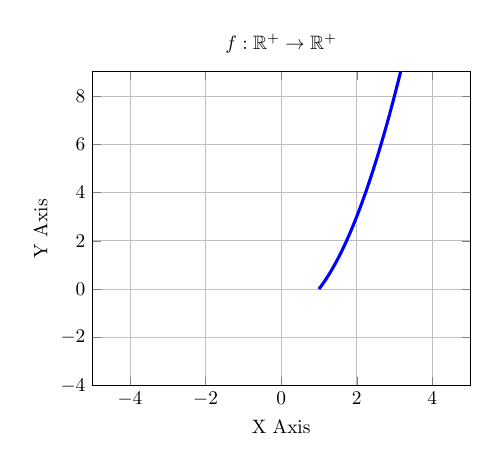
\begin{tikzpicture}[scale=0.7]
            \begin{axis}[
                xmax=5,
                xmin=-5,
                ymax=9,
                ymin=-4,
                samples=50,
                grid=major,
                xlabel={X Axis},
                ylabel={Y Axis},
                title={$f:\mathbb{R}^+\rightarrow\mathbb{R}^+$}
            ]
            \addplot[blue,ultra thick,domain=1:5](x,x^2-1);
        \end{axis}
        \end{tikzpicture}
        \label{sketch:exm-1}
    \end{subfigure}
    \hfill
    \begin{subfigure}[ht]{0.47\textwidth}
        \centering
        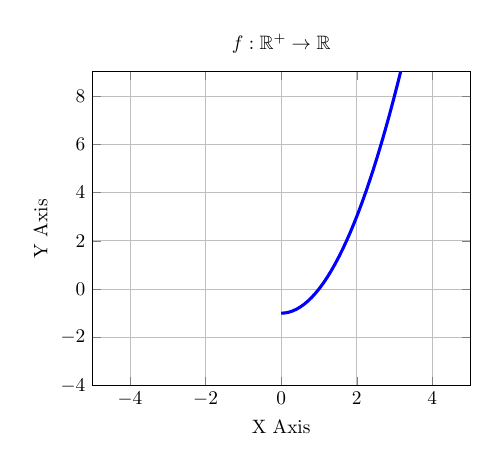
\begin{tikzpicture}[scale=0.7]
            \begin{axis}[
                xmax=5,
                xmin=-5,
                ymax=9,
                ymin=-4,
                samples=50,
                grid=major,
                xlabel={X Axis},
                ylabel={Y Axis},
                title={$f:\mathbb{R}^+\rightarrow\mathbb{R}$}
            ]
            \addplot[blue,ultra thick,domain=0:5](x,x^2-1);
        \end{axis}
        \end{tikzpicture}
        \label{sketch:exm-2}
    \end{subfigure}
    \vfill
    \begin{subfigure}[ht]{0.47\textwidth}
        \centering
        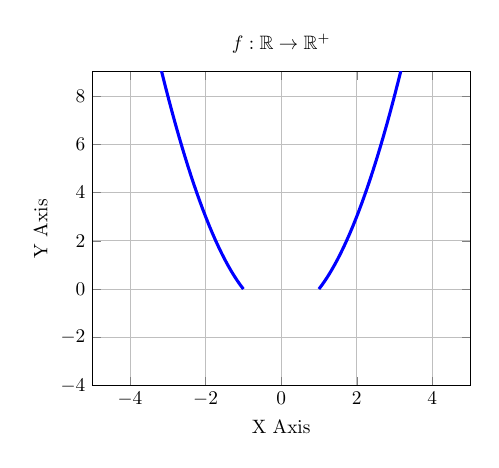
\begin{tikzpicture}[scale=0.7]
            \begin{axis}[
                xmax=5,
                xmin=-5,
                ymax=9,
                ymin=-4,
                samples=50,
                grid=major,
                xlabel={X Axis},
                ylabel={Y Axis},
                title={$f:\mathbb{R}\rightarrow\mathbb{R}^+$}
            ]
            \addplot[blue,ultra thick,domain=-5:-1](x,x^2-1);
            \addplot[blue,ultra thick,domain=1:5](x,x^2-1);
        \end{axis}
        \end{tikzpicture}
        \label{sketch:exm-3}
    \end{subfigure}
    \hfill
    \begin{subfigure}[ht]{0.47\textwidth}
        \centering
        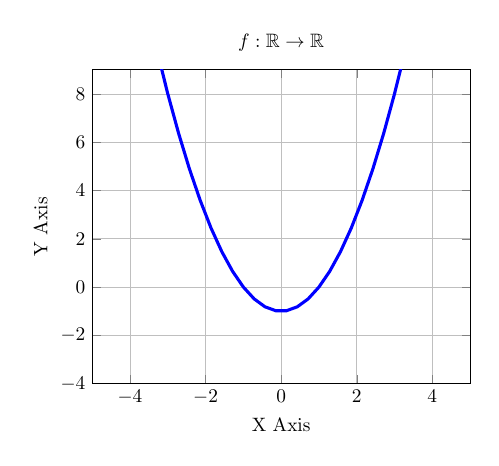
\begin{tikzpicture}[scale=0.7]
            \begin{axis}[
                xmax=5,
                xmin=-5,
                ymax=9,
                ymin=-4,
                samples=50,
                grid=major,
                xlabel={X Axis},
                ylabel={Y Axis},
                title={$f:\mathbb{R}\rightarrow\mathbb{R}$}
            ]
            \addplot[blue, ultra thick,domain=-5:9](x,x^2-1);
        \end{axis}
        \end{tikzpicture}
        \label{sketch:exm-4}
    \end{subfigure}
\end{figure}


% === End Section Includes ====

\newpage

\medskip
\printbibliography

\end{document}
